% concatenated from rational_quivers_arxiv.tex
\documentclass[a4paper,12pt,reqno]{amsart}
\usepackage{amsmath}
\usepackage{amssymb}
\usepackage{amsfonts}
\usepackage{amscd}
\usepackage{amsthm}
\usepackage{mathrsfs}
\usepackage{tikz}
\usetikzlibrary{arrows, cd, positioning, shapes}
\tikzset{
    every node/.style={inner sep=2pt},
    arr/.style={thin, -{Stealth[scale=1.0]}},
    revarr/.style={thin, {Stealth[scale=1.0]}-},
    loopstyle/.style={thin, -{Stealth[scale=1.0]},
        loop left, min distance=1.5cm, out=135, in=225, distance=1.5cm
    }
}
\tikzcdset{arrow style=tikz}

\usepackage[all]{xy}
\usepackage[bb=boondox,bbscaled=.95,cal=boondoxo]{mathalfa}
\usepackage[numbers]{natbib}
\usepackage[a4paper, margin=2cm]{geometry}
\usepackage{hyperref}

\newcommand{\HH}{{\rm\bf H}}
\newcommand{\CC}{{\rm\bf C}}
\newcommand{\RR}{{\rm\bf R}}
\newcommand{\QQ}{{\rm\bf Q}}
\newcommand{\ZZ}{{\rm\bf Z}}
\newcommand{\NN}{{\rm\bf N}}
\newcommand{\GG}{{\rm\bf G}}
\newcommand{\FF}{{\rm\bf F}}
\newcommand{\EE}{{\rm\bf E}}
\newcommand{\PP}{{\rm\bf P}}
\newcommand{\Adeles}{{\rm\bf A}}

\newcommand{\OO}{\mathcal{O}}

\DeclareMathOperator{\absNorm}{\mathfrak{N}}

\DeclareMathOperator{\Spec}{\mathrm{Spec}}
\DeclareMathOperator{\Specm}{\mathrm{Specm}}
\DeclareMathOperator{\Spc}{\mathrm{Spc}}
\DeclareMathOperator{\diag}{\mathrm{diag}}
\DeclareMathOperator{\Gm}{\mathrm{{\bf G}_m}}
\DeclareMathOperator{\GL}{\mathrm{GL}}
\DeclareMathOperator{\SL}{\mathrm{SL}}
\DeclareMathOperator{\PGL}{\mathrm{PGL}}
\DeclareMathOperator{\PSL}{\mathrm{PSL}}
\DeclareMathOperator{\Oo}{\mathrm{O}}
\DeclareMathOperator{\U}{\mathrm{U}}
\DeclareMathOperator{\SO}{\mathrm{SO}}
\DeclareMathOperator{\SU}{\mathrm{SU}}
\DeclareMathOperator{\Sp}{\mathrm{Sp}}
\DeclareMathOperator{\Z}{\mathrm{Z}}
\DeclareMathOperator{\Mod}{{\mathcal M}\!\textit{od}}
\DeclareMathOperator{\Aut}{\mathrm{Aut}}
\DeclareMathOperator{\End}{\mathrm{End}}
\DeclareMathOperator{\Hom}{\mathrm{Hom}}
\DeclareMathOperator{\iEnd}{\mathcal E\textit{nd}\,}
\DeclareMathOperator{\iHom}{\mathcal H\!\textit{om}\,}
\DeclareMathOperator{\Gr}{\mathrm{Gr}}
\DeclareMathOperator{\Diff}{{\mathcal D\!\textit{i}\textit{f}\textit{f}\,}}
\DeclareMathOperator{\Der}{{\mathcal D\!\textit{\'e}\textit{r}}}
\DeclareMathOperator{\D}{{\mathcal D}}
\DeclareMathOperator{\Pp}{{\mathcal P}}
\DeclareMathOperator{\kernel}{\mathrm{ker}}
\DeclareMathOperator{\image}{\mathrm{im}}
\DeclareMathOperator{\rank}{\mathrm{rank}}
\DeclareMathOperator{\tr}{\mathrm{tr}}
\DeclareMathOperator{\Gal}{\mathrm {Gal}}
\DeclareMathOperator{\Sym}{\mathrm {Sym}}
\DeclareMathOperator{\ind}{\mathrm{Ind}}
\DeclareMathOperator{\res}{\mathrm{Res}}
\DeclareMathOperator{\Ad}{\mathrm{Ad}}
\DeclareMathOperator{\ad}{\mathrm{ad}}
\DeclareMathOperator{\der}{\mathrm{der}}
\DeclareMathOperator{\id}{\mathrm{id}}
\DeclareMathOperator{\Lie}{\mathrm{Lie}}
\DeclareMathOperator{\HC}{\mathrm{HC}}
\DeclareMathOperator{\Rep}{\mathrm{Rep}}
\newcommand{\zentrum}{\mathscr{C}}

\newcommand{\liea}{{\mathfrak {a}}}
\newcommand{\lieb}{{\mathfrak {b}}}
\newcommand{\liec}{{\mathfrak {c}}}
\newcommand{\lied}{{\mathfrak {d}}}
\newcommand{\lieg}{{\mathfrak {g}}}
\newcommand{\lieh}{{\mathfrak {h}}}
\newcommand{\liek}{{\mathfrak {k}}}
\newcommand{\liel}{{\mathfrak {l}}}
\newcommand{\lien}{{\mathfrak {n}}}
\newcommand{\lies}{{\mathfrak {s}}}
\newcommand{\liet}{{\mathfrak {t}}}
\newcommand{\lieo}{{\mathfrak {o}}}
\newcommand{\liep}{{\mathfrak {p}}}
\newcommand{\lieq}{{\mathfrak {q}}}
\newcommand{\lier}{{\mathfrak {r}}}
\newcommand{\lieu}{{\mathfrak {u}}}
\newcommand{\liex}{{\mathfrak {x}}}
\newcommand{\liey}{{\mathfrak {y}}}
\newcommand{\liez}{{\mathfrak {z}}}
\newcommand{\liegl}{{\mathfrak {gl}}}
\newcommand{\liesl}{{\mathfrak {sl}}}
\newcommand{\lieso}{{\mathfrak {so}}}
\newcommand{\liesu}{{\mathfrak {su}}}

\newcommand{\characteristic}{\mathrm {char\,}}
\DeclareMathOperator{\vol}{\mathrm {vol}}
\DeclareMathOperator{\sgn}{\mathrm {sgn}}

\DeclareMathOperator*{\Otimes}{\ensuremath{\otimes}}

\newcommand{\absnorm}[1]{\ensuremath{\left|\!\left|{#1}\right|\!\right|}}

\newcommand{\mmod}{\mathrm {mod\,}}

\newcommand{\adots}{\ensuremath{
\put(-3,-6){\normalsize$\,$}
\put(-2.2,-3.5){\normalsize$\cdot$}
\cdot
\put(-1.0,3.5){\normalsize$\cdot$}
\put(0.0,6){\normalsize$\,$}
}}

\theoremstyle{plain}
\newtheorem{theorem}{Theorem}[section]
\newtheorem{lemma}[theorem]{Lemma}
\newtheorem{corollary}[theorem]{Corollary}
\newtheorem{proposition}[theorem]{Proposition}

\theoremstyle{remark}
\newtheorem{remark}[theorem]{Remark}
\newtheorem{definition}[theorem]{Definition}
\newtheorem{example}[theorem]{Example}

\bibpunct{[}{]}{,}{n}{}{,}


\begin{document}

    \title{Rational structures on quivers\\and a generalization of Gelfand's equivalence}

    \author{Fabian Januszewski}
    \address{Institut f\"ur Mathematik, Fakult\"at EIM, Paderborn University, Warburger Str.\ 100, 33098 Paderborn, Germany}
    \email{fabian.januszewski@math.uni-paderborn.de}
    \subjclass[2010]{Primary: 16G20; Secondary: 22E47}

    \begin{abstract}
      We introduce the notion of rational structure on a quiver and associated representations to establish a coherent framework for studying quiver representations in separable field extensions. This notion is linked to a refinement of the notion of $K$-species, which we term \'etale $K$-species: We establish a categorical anti-equivalence between the category of $K$-rational quivers and that of \'etale $K$-species, which extends to an equivalence of their respective representation categories.

      For $K$-rational quivers there is a canonical notion of base change, which suggests a corresponding notion of base change for (\'etale) $K$-species which we elaborate.

      As a primary application, we generalize Gelfand's celebrated equivalence between certain blocks of Harish-Chandra modules for $\mathrm{SL}_2(\mathbb{R})$ and representations of the Gelfand quiver to a rational setting. To this end, we define a $\mathbb{Q}$-rational structure on the Gelfand quiver and its representations. A key technical tool, which we call unipotent stabilization, is developed to construct the functor from certain rational Harish-Chandra modules to nilpotent rational quiver representations. We prove that this functor is an equivalence. A similar result is established for the cyclic quiver. A notable consequence of this rational framework is that the defining relation of the Gelfand quiver becomes superfluous when working over fields not containing $\sqrt{-1}$. This allows us to recast our results in the language of $\QQ$-species without relations.
    \end{abstract}

    \maketitle

    {\tiny
      \tableofcontents
    }

    %\addcontentsline{toc}{section}{Introduction}
    \section*{Introduction}

    Since the pioneering work of Gabriel \cite{Gabriel1972}, the representation theory of quivers is well understood over algebraically closed fields. For general non-algebraically closed fields, by the foundational work of Dlab and Ringel \cite{DlabRingel1975,DlabRingel1976}, the notion $K$-species is a suitable generalization of quivers. Within this framework the passage from a non-algebraically closed field to an algebraically closed field is very useful and at times essential in certain arguments.

    In the first half of our work, we build a coherent framework which allows for the study of quiver representations over non-algebraically closed fields on the one hand, and which on the other hand admits a suitable notion of base change for passage to (potentially algebraically closed) field extensions.

    The underlying concept is that of a rational structure on a quiver and associated representations. A central theme is to relate this notion to a suitable refinement of the well known concept of $K$-species.

    In this context, we introduce the notion of {\em \'etale $K$-species} and establish a categorical anti-equivalence between the category of $K$-rational quivers and the category of \'etale $K$-species (Theorem \ref{thm:KrationalquiveretaleKspeciesantiequivalence}). This structural result is complemented by a corresponding equivalence between the respective categories of representations (Theorem \ref{thm:species_equivalence}).

    The natural notion of base change for $K$-rational quivers has a natural analogue for \'etale $K$-species, which in turn suggests a general analogue for the notion of base change for general $K$-species (cf.\ Remark \ref{rmk:simplealgebraspecies}). As is expected, restriction and base change for $K$-rational quivers and \'etale $K$-species form adjoint pairs of functors (Propositions \ref{prop:quiverrestrictionbasechangeadjunction} and \ref{prop:speciesrestrictionbasechangeadjunction}).

    \smallskip
    With a view towards applications in representation theory, we apply this framework to the study of rational Harish-Chandra modules for $\SL_2(\RR)$. Motivated by (expected) rationality and integrality properties of automorphic $L$-functions of (hypothetical) motivic origin, a rational theory of Harish-Chandra modules was developed by G\"unter Harder, Michael Harris and the author (cf.\ \cite{HarderRaghuram-Book}, \cite{Harris2012,Harris2020Erratum}, \cite{Januszewski18}).

    In I.~M.~Gelfand's influential 1972 ICM adress, Gelfand observed that the category of nilpotent complex representations of the quiver with relation
    \begin{center}
    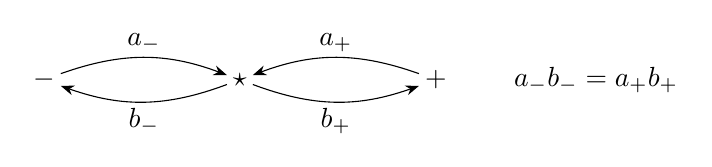
\begin{tikzpicture}[baseline=(current bounding box.center)]
    \node (A) {$-$};
    \node (B) [right=6em of A] {$\star$};
    \node (C) [right=6em of B] {$+$};
    \node (D) [right=2em of C] {$a_{-} b_{-} = a_{+} b_{+}$};
    \draw [arr, bend left=20] (A) to node [midway, above] {$a_-$} (B);
    \draw [arr, bend left=20] (B) to node [midway, below] {$b_-$} (A);
    \draw [arr, bend right=20] (B) to node [midway, below] {$b_+$} (C);
    \draw [arr, bend right=20] (C) to node [midway, above] {$a_+$} (B);
    \end{tikzpicture}
    \end{center}
    which now bears his name, is equivalent to the blocks $\HC_\lambda(\liesl_2,\SO(2))$ of Harish-Chandra modules for $\SL_2(\RR)$ which contain the $\sqrt{\lambda}$-dimensional irreducible representation of $\SL_2$.

    We generalize Gelfand's equivalence to arbitrary fields of characteristic $0$. To achieve this, we first define a $\QQ$-rational structure on Gelfand's quiver (and the cyclic quiver) and obtain a $\QQ$-rational quiver $\Gamma_\QQ$ (cf.\ Examples \ref{ex:gelfand} and \ref{ex:cyclic}). The associated \'etale $\QQ$-species is the following $\QQ$-species $S_{\rm Gelfand}$:
    \begin{center}
    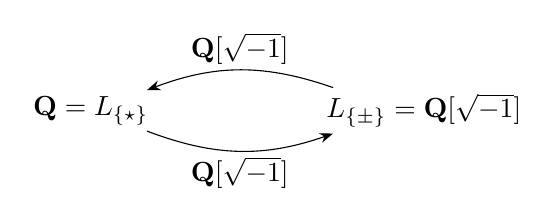
\begin{tikzpicture}[baseline=(current bounding box.center)]
    \node (Mstar) {$\QQ=L_{\{\star\}}$};
    \node (M+)    [right=4em of Mstar] {$\quad\quad L_{\{\pm\}}=\QQ[\sqrt{-1}]$};
    \draw [arr, bend right=20] (Mstar) to node [below] {$\QQ[\sqrt{-1}]$} (M+);
    \draw [arr, bend right=20] (M+) to node [above] {$\QQ[\sqrt{-1}]$} (Mstar);
    \end{tikzpicture}
    \end{center}
    Here the $\QQ,\QQ[\sqrt{-1}]$- and $\QQ[\sqrt{-1}],\QQ$-bimodules
    \[
      {}_{\{\star\}}M_{\{\pm\}}=\QQ[\sqrt{-1}],\quad
      {}_{\{\pm\}}M_{\{\star\}}=\QQ[\sqrt{-1}],
    \]
    carry the natural bimodule structures. In the case of the cyclic quiver the bimodule structure turns out to be slightly more interesting (cf.\ Example \ref{ex:cyclic}).

    The construction of a $\QQ$-rational structure on a quiver representation associated with a Harish-Chandra module is non-trivial and generally requires a procedure which we term {\em unipotent stabilization} (see Subsection \ref{sec:unipotentstabilization}). The properties of unipotent stabilization play a central role not only in the construction itself but also in the proof of our main result, Theorem \ref{thm:EEQQequivalence}, and its counterpart for the cyclic quiver, Theorem \ref{thm:cyclicEEQQequivalence}, for the case $\ell=0$.

    For $\lambda=\ell^2\geq 1$, we establish the desired equivalence of abelian categories:
    \begin{equation}
      \EE_\QQ\colon\HC_\lambda(\liesl_2,\SO(2))_\QQ \simeq \Rep^{\mathrm{nil}}(\Gamma_\QQ).
      \label{eq:HCquiverequivalence}
    \end{equation}
    Here, $\HC_\lambda(\liesl_2,\SO(2))_\QQ$ denotes the block of $\QQ$-rational Harish-Chandra modules with generalized infinitesimal character $\lambda$ containing the irreducible $\ell$-dimensional representation of $\SL_2$. On the right hand side of \eqref{eq:HCquiverequivalence}, $\Rep^{\mathrm{nil}}(\Gamma_\QQ)$ is the category of nilpotent, finite-dimensional, $\QQ$-rational representations of the Gelfand quiver, endowed with a suitable $\QQ$-rational structure (cf. Example \ref{ex:gelfand}).

    Combining this result with Theorem \ref{thm:species_equivalence} on the equivalence of $\QQ$-rational quiver representations and \'etale $\QQ$-species representations, we obtain the equivalence
    \begin{equation}
      \EE_\QQ\colon\HC_\lambda(\liesl_2,\SO(2))_\QQ \simeq \Rep^{\mathrm{nil}}(S_{\rm Gelfand}).
      \label{eq:HCspeciesequivalence}
    \end{equation}
    
    The equivalence \eqref{eq:HCquiverequivalence} generalizes to an equivalence over arbitrary fields $E$ of characteristic zero (Remark \ref{rmk:generalbases}):
    \[
    \EE_E\colon\HC_\lambda(\liesl_2,\SO(2))_E \simeq \Rep^{\mathrm{nil}}(\Gamma_E).
    \]
    The equivalence \eqref{eq:HCspeciesequivalence} generalizes to an equivalence over arbitary fields $E$ of characteristic zero as well: For any field $E$ of characteristic $0$ we have
    \[
      \EE_E\colon\HC_\lambda(\liesl_2,\SO(2))_E \simeq \Rep^{\mathrm{nil}}(S_{\rm Gelfand}\otimes_\QQ E).
    \]
    We emphasize that the species $S_{\rm Gelfand}\otimes_\QQ E$ changes structurally if $\sqrt{-1}\in E$, base change being a non-trivial operation for (\'etale) $K$-species (cf.\ Definition \ref{def:basechangeforspecies}). Moreover, a relation has to be added whenever $\sqrt{-1}\in E$.

    It is remarkable that whenever $\sqrt{-1}\not\in E$, then neither the $E$-rational Gelfand quiver, nor the corresponding \'etale $E$-species, need to be equipped with a relation. The rationality properties render the defining relation $a_{-} b_{-} = a_{+} b_{+}$ superfluos.
    
    Finally, in Section \ref{sec:examples}, we illustrate our main equivalence with a handful of fundamental examples, including finite-dimensional representations, discrete series, and principal series representations, and describe their corresponding quiver and species representations.

\medskip    
%\addcontentsline{toc}{subsection}{Acknowledgements}
\noindent{\bf Acknowledgements.}
The author thanks Igor Burban and William Crawley-Boevey for fruitful discussions. The author acknowledges support by the Deutsche Forschungsgemeinschaft (DFG, German Research Foundation) -- SFB-TRR 358/1 2023 -- 491392403.


%\addcontentsline{toc}{section}{Notation}

\subsection*{Notation}

All homomorphisms of commutative rings are assumed to be unitial. Let $K$ denote a field and let $V$ and $W$ denote right and left $K$-vector spaces respectively. Then $V\otimes_K W$ denotes the respective tensor product. If $L$ is another field and if $V$ carries an $L,K$-bimodule structure, then $V\otimes_KW$ is canonically a left $L$-vector space and likewise for $W$. Moreover, if $\sigma\colon K\to L$ is a ring homomorphism, then for any right vector space $V$ and any $L$-vector space $W$ we consider the twisted tensor product $V\otimes_{K,\sigma}W$, where for all $a\in K$ and any $v\in V$, $w\in W$:
\[
va\otimes w=v\otimes\sigma(a)w.
\]
Similarly, if $V$ is a right $L$-vector space, and $W$ a left $K$-vector space, we understand $V\otimes_{\sigma,K}W$ via the analogous relation
\[
v\otimes aw=v\sigma(a)\otimes w.
\]
For a finite or infinite Galois extension $L/K$ of fields we write $\Gal(L/K)$ for the Galois group with the profinite topology. I.\,e.\ if $L/K$ is finite, then $\Gal(L/K)$ is discrete. All $\Gal(L/K)$-modules are considered continuous with the target being topologized discretely.

\section{Rational structures on quivers}\label{sec:rationalstructures}

Since Galois descent plays a central role, we recall some well-known concepts and statements.

\subsection{Galois descent}

Let $L/K$ be a finite or infinite Galois extension with Galois group $\Gal(L/K)$. For $\sigma\in\Gal(L/K)$ and $\alpha\in L$, we sometimes write $\alpha^\sigma=\sigma(\alpha)$, even though it is strictly speaking a left action.

Let $V, W$ be $L$-vector spaces. The Galois group $\Gal(L/K)$ acts (continously) on the (discrete) set of $L$-linear maps $\Hom_L(V,W)$ via
\[
\forall\sigma\in\Gal(L/K),\,\phi\in\Hom_L(V,W)\colon\quad \phi^\sigma:=\sigma\circ\phi\circ\sigma^{-1}.
\]

We call a map $\phi\colon V\to W$ {\em semi-linear} with respect to a given $\sigma\in\Gal(L/K)$, or simply $\sigma$-linear, if for all $v\in V$ and all $\alpha\in L$:
\[
\phi(\alpha\cdot v)=\sigma(\alpha)\phi(v).
\]

Every $L$-vector space $V$ can be considered as a $K$-vector space via the embedding $K\to L$. A {\em $K$-structure} on an $L$-vector space $V$ is a group homomorphism
\[
\varphi\colon\Gal(L/K)\to\Aut_K(V),\;\sigma\mapsto\varphi_\sigma
\]
with the property that for each $\sigma\in\Gal(L/K)$, the map
\[
\varphi_\sigma\colon V\to V
\]
is $\sigma$-linear. In the following, we identify $\varphi$ with the collection $\varphi_\bullet=(\varphi_\sigma)_{\sigma\in\Gal(L/K)}$.

We call a map $\phi\in\Hom_L(V,W)$ between two $L$-vector spaces with $K$-structure {\em $K$-rational} if $\phi$ commutes with the two given actions of $\Gal(L/K)$ on $V$ and $W$.

If $V$ is a $K$-vector space, then $L\otimes_K V$ carries a canonical $K$-structure, which is explicitly given by
\[
\varphi_\sigma(\alpha\otimes v)=\sigma(\alpha)\otimes v,\quad \sigma\in\Gal(L/K),\,\alpha\in L,\,v\in V.
\]
Every $K$-linear map $\phi\colon V\to W$ then induces a $K$-rational map ${\bf1}\otimes\phi\colon L\otimes V\to L\otimes W$.

The following result is well known:

\begin{theorem}[Galois descent]\label{thm:galoisdescent}
  Let $L/K$ be a finite or infinite Galois extension. The category $\rm{Vec}_K$ of $K$-vector spaces is equivalent, via the functor
  \[
  V\;\mapsto\; \left(L\otimes_K V,(\varphi_\sigma)_{\sigma}\right)
  \]
  to the category of $L$-vector spaces with a $K$-rational structure and $K$-rational maps as morphisms. A quasi-inverse functor is given by
  \[
  \left(V,(\varphi_\sigma)_\sigma\right)\;\mapsto\;V^{\Gal(L/K)}:=\{v\in V\mid\forall\sigma\in\Gal(L/K)\colon \varphi_\sigma(v)=v\}.
  \]
\end{theorem}

\subsection{Rational structures on quivers}

\begin{definition}[Quiver (Gabriel)]
  A (classical) quiver is a quadruple $\Gamma=(V,E,s,t)$ consisting of a finite set of vertices $V$, a finite set of edges $E$, and two maps $s,t\colon E\to V$, which assign to each edge $e\in E$ a source $s(e)\in V$ and a target $t(e)\in V$.
\end{definition}

\begin{definition}[$K$-rational (\'etale) quivers]\label{def:rationalquivers}
  An {\em (\'etale) $K$-rational structure} on a quiver $\Gamma=(V,E,s,t)$ is a group homomorphism $\rho\colon\Gal(L/K)\to\Aut(\Gamma)$ into the automorphism group of $\Gamma$ for a Galois extension $L/K$ with Galois group $\Gal(L/K)$, such that the actions of $\Gal(L/K)$ on $V$ and $E$ induced by $\rho$ are continuous when $V$ and $E$ are considered as discrete sets. We write $\Gamma_K:=(\Gamma,\rho)$ for the quiver $\Gamma$ endowed with the rational structure $\rho$. We say that $\Gamma_K$ is an {\em (\'etale) quiver over $K$}.
\end{definition}

\begin{definition}[Split rational quivers]\label{def:splitrationalquivers}
  We call a quiver $\Gamma_K=(\Gamma,\rho)$ over $K$ {\em constant} or {\em split over $K$} if $\rho$ is the trivial group homomorphism, i.\,e.\ if the $\Gal(L/K)$ actions on $V$ and $E$ are both trivial.
\end{definition}

\begin{remark}
A $K$-rational quiver is a diagram in the category of finite $\Gal(L/K)$-sets:
   \begin{center}
   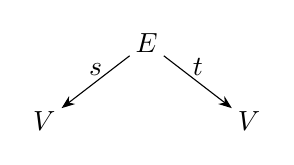
\begin{tikzpicture}[>=Stealth]
    \node (E) at (0,1) {$E$};
    \node (V_left) at (-1.3,0) {$V$};
    \node (V_right) at (1.3,0) {$V$};
    \draw[->] (E) -- node[above] {$s$} (V_left);
    \draw[->] (E) -- node[above] {$t$} (V_right);
    \end{tikzpicture}
   \end{center}
\end{remark}

\begin{remark}
Specifically, a $K$-rational structure $\rho$ on a quiver $\Gamma=(V,E,s,t)$ is given by:
\begin{itemize}
\item[(i)] A (continuous left) $\Gal(L/K)$-action
  \[\rho_V\colon\Gal(L/K)\to\Sym(V)\] on the set of vertices $V$,
  \item[(ii)] a (continuous left) $\Gal(L/K)$-action \[\rho_E\colon\Gal(L/K)\to\Sym(E)\] on the set of edges,
\end{itemize}
such that $s$ and $t$ are homomorphisms of $\Gal(L/K)$-sets, i.\,e., the following compatibilities must be satisfied: For all $\sigma\in\Gal(L/K)$ and all edges $e\in E$ it holds that
\begin{equation}
  s(\sigma e)=\sigma s(e)\quad\text{and}\quad t(\sigma e)=\sigma t(e).
  \label{eq:stgaloisequivariance}
\end{equation}
In other words: We reformulated Gabriel's original definition in the category of (continuous discrete) $\Gal(L/K)$-sets.
\end{remark}

\begin{remark}[Relations]
  If $\Gamma$ is a quiver with relations, we require that the Galois action respects them, i.e., that each element of the Galois group maps a given relation to a given relation or, equivalently, that the image of $\rho$ lies in the automorphism group of the quiver $\Gamma$ with relations.
\end{remark}

\begin{remark}
  Let $K^{\rm sep}$ denote a separable algebraic closure of $K$. Then any of the Galois groups $\Gal(L/K)$ occuring in Definition \ref{def:rationalquivers} may be (non-canonically) considered as a quotient of the absolute group $\Gal(K^{\rm sep}/K)$. Therefore all actions in Definition \ref{def:rationalquivers} arise from continuous actions of $\Gal(K^{\rm sep}/K$ on $E$ and $V$. $E$ and $V$ being finite, any $K$-rational structure on the quiver $\Gamma$ factors over a finite quotient $\Gal(K^{\rm sep}/K)\to\Gal(L_0/K)$ with $L_0/K$ a finite Galois extension. Therefore we may often assume that $L/K$ is a finite Galois extensions without loss of generality.

  That being said, in certain situations, such as when considering categorical aspects of $K$-rational quivers, the discussion simplifies if we consider $\Gal(K^{\rm sep}/K)$-actions, as is the case in the following definition.
\end{remark}

\begin{definition}[Rational homomorphisms of quivers]\label{def:rationalquiverhom}
  A homomorphism $\phi\colon\Gamma_K\to \Gamma_K'$ of two quivers $\Gamma_K$ and $\Gamma_K'$ over $K$ is a homomorphism of quivers $\phi\colon\Gamma\to\Gamma'$ which commutes with the $\Gal(K^{\rm sep}/K)$-Galois actions on $\Gamma_K$ and $\Gamma_K'$.
\end{definition}

\begin{definition}[Base change]\label{def:quiverbasechange}
  For any quiver $\Gamma_K=(\Gamma,\rho)$ with rational structure given by an action of $\Gal(L/K)$, we have for any intermediate field $L/E/K$, $E/K$ finite, the $E$-rational quiver
  \[
  \Gamma_E=E\otimes_K\Gamma_K:=(\Gamma,\rho|_{\Gal(L/E)}),
  \]
  which we call the {\em base change} of $\Gamma_K$ to $E$.
\end{definition}

\begin{remark}
  If $\Gamma$ is a quiver and $L/K$ is a Galois extension, then all isomorphism classes of $K$-rational structures on $\Gamma$ can be classified using Galois cohomology
  \[
  H^1(\Gal(K^{\rm sep}/K);\Aut(\Gamma)).
  \]
  Here, we can assume without loss of generality that $\Aut(\Gamma)$ is endowed with the trivial Galois action. If $\Aut(\Gamma)$ is abelian, it follows in particular that
  \[
  H^1(\Gal(K^{\rm sep}/K);\Aut(\Gamma))=\Hom(\Gal(K^{\rm sep}/K),\Aut(\Gamma)).
  \]
\end{remark}

\begin{definition}[Restriction]\label{def:quiverrestriction}
  For any intermediate field $L/E/K$, $E/K$ finite, and any $E$-rational quiver $\Gamma_E=(\Gamma,\rho)$, with $\Gamma=(V,E,s,t)$ we consider the quiver
  \begin{align*}
    \res_{E/K}\Gamma_E=(&\Gal(L/K)\times_{\Gal(L/E)}V,\\
    &\Gal(L/K)\times_{\Gal(L/E)}E,\\
    &\Gal(L/K)\times_{\Gal(L/E)}s,\\
    &\Gal(L/K)\times_{\Gal(L/E)}t\,)
  \end{align*}
  which we call the {\em restriction} of $\Gamma_E$ to $K$.
\end{definition}

\begin{proposition}\label{prop:quiverrestrictionbasechangeadjunction}
  For any intermediate field $L/E/K$, $E/K$ finite, and any $E$-rational quiver $\Gamma_E=(\Gamma,\rho)$, and any $K$-rational quiver $\Gamma_K'$, we have a natural isomorphism
  \begin{equation}
    \Hom_{E}(\Gamma_E,E\otimes_K\Gamma_K')\cong
    \Hom_{K}(\res_{E/K}\Gamma_E,\Gamma_K').
  \end{equation}
\end{proposition}

\begin{proof}
  This is an elementary application of the universal property of the functor
  \[
  \Gal(L/K)\times_{\Gal(L/E)}(-)\colon \{\text{finite $\Gal(L/E)$-sets}\}\to\{\text{finite $\Gal(L/K)$-sets}\},
  \]
  which is left adjoint to the forgetful functor
  \[
  \{\text{finite $\Gal(L/K)$-sets}\}\to\{\text{finite $\Gal(L/M)$-sets}\}.
  \]
\end{proof}

\begin{remark}
  We remark that quivers over finite fields $\FF_q$ together with an automorphism (of order $2$) have been previously studied in \cite{DengDuParshallWang2008} in the context of quantum groups.
\end{remark}

\subsection{Rational quiver representations}\label{sec:rationalquiverrepresentations}

  \begin{definition}[Representations of rational quivers]\label{def:rationalrepresentations}
    Let $\Gamma_K$ be a quiver over $K$ with respect to a Galois extension $L/K$. A ($K$-rational) {\em representation} $M_K$ of $\Gamma_K$ consists of:
    \begin{itemize}
    \item[(i)]
      A family $M=(M(v))_{v\in V}$ of $L$-vector spaces.
    \item[(ii)] Semi-linear isomorphisms $\varphi_{v,\sigma}\colon M(v)\to M(\sigma v)$ for each $v\in V$ and $\sigma\in\Gal(L/K)$ such that the cocycle condition
      \begin{equation}
        \varphi_{\tau v,\sigma}\circ\varphi_{v,\tau}=\varphi_{v,\sigma\tau}
        \label{eq:semi-linearactiononrep}
      \end{equation}
      is satisfied.
    \item[(iii)] A classical quiver representation of $\Gamma$ on $M$, i.e., for each edge $e\in E$, an $L$-linear map $\phi_e\colon M(s(e))\to M(t(e))$ is given, which is compatible with the Galois action in the following sense:
      For each edge $e\in E$ and each $\sigma\in\Gal(L/K)$, we have
      \begin{equation}
        \phi_{\sigma e}\circ\varphi_{s(e),\sigma}=\varphi_{t(e),\sigma}\circ\phi_e.
        \label{eq:koecheractiononrep}
      \end{equation}
    \end{itemize}
  \end{definition}

  \begin{definition}[Homomorphisms of rational quiver representations]\label{def:rationalrepresentationhom}
    A {\em homomorphism} of $K$-rational representations $M=(M(v))_v$, $N=(N(v))_v$ is a classical homomorphism $\left(\psi_v\colon M(v)\to N(v)\right)_v$ over $L$, which is compatible with the rational structures on $M$ and $N$: For all $v\in V$ and all $\sigma\in\Gal(L/K)$, we have
    \begin{equation}
      \psi_{\sigma v}\circ\varphi_{v,\sigma}=\varphi_{v,\sigma}\circ\psi_v.
      \label{eq:koecheractiononrephom}
    \end{equation}
  \end{definition}
  
  \begin{remark}
    Semi-linearity in point (ii) means specifically
    \begin{equation}
      \varphi_{v,\sigma}(a\cdot m)=\sigma(a)\cdot\varphi_{v,\sigma}(m)
    \end{equation}
    for all $v\in V$, $m\in M(v)$, $a\in L$ and $\sigma\in\Gal(L/K)$.
  \end{remark}

  \begin{definition}
    For a $K$-rational quiver $\Gamma_K$, we define $\Rep(\Gamma_K)$ as the category of finite-dimensional $K$-rational representations of $\Gamma_K$. Moreover we define the full subcategory $\Rep^{\rm nil}(\Gamma_K)$ in $\Rep(\Gamma_K)$ consisting of finite-dimensional {\em nilpotent} $K$-rational representations of $\Gamma_K$.
  \end{definition}

  \begin{proposition}[Base change for representations]
    If $M_K$ is a (nilpotent) representation of a $K$-rational quiver $\Gamma_K$, then for any intermediate field $L/E/K$, the $E$-vector space $M_E:=E\otimes_KM_K$ carries a natural structure as a (nilpotent) representation of the base change $E\otimes_K\Gamma_K$. Base change of (nilpotent) representations is functorial.
  \end{proposition}

  \begin{proof}
    This follows by $E$-linear extension from the definitions.
  \end{proof}

  \begin{remark}
    Considering everything over the absolute Galois group $\Gal(K^{\rm sep}/K)$, we see that $(\Rep(\Gamma_E))_{K\subseteq E\subseteq K^{\rm sep}}$ and $(\Rep^{\rm nil}(\Gamma_E))_{K\subseteq E\subseteq K^{\rm sep}}$ define stacks in the \'etale topology on $K$.
  \end{remark}

\subsection{Base change for Hom}

  \begin{proposition}\label{prop:homdescent}
    Let $\Gamma_K$ be a quiver with a $K$-rational structure. For $K$-rational representations $M_K$ and $N_K$ of $\Gamma_K$, we have for any intermediate field $L/E/K$ a canonical isomorphism
    \begin{equation}
      E\otimes_K\Hom_{\Gamma_K}(M_K,N_K) \cong \Hom_{\Gamma_E}(M_E,N_E)
    \end{equation}
    of finite-dimensional $E$-vector spaces.
  \end{proposition}

  \begin{proof}
    We first consider the case $E=L$. We aim to show the existence of a canonical isomorphism of $L$-vector spaces
    \[
    L\otimes_K\Hom_{\Gamma_K}(M_K,N_K) \cong \Hom_{\Gamma}(M, N),
    \]
    where $\Hom_{\Gamma}(M, N)$ denotes the space of homomorphisms of the underlying classical quiver representations over $L$.
    
    Let $G = \Gal(L/K)$. We consider the $L$-vector space $W := \Hom_{\Gamma}(M, N)$. An element $\psi \in W$ is a collection of $L$-linear maps $\psi = (\psi_v)_{v\in V}$ such that for every edge $e \in E$, we have $\psi_{t(e)}\circ \phi_{e,M} = \phi_{e,N}\circ\psi_{s(e)}$.
    
    We define a semilinear action of $G$ on $W$. For $\sigma \in G$ and $\psi \in W$, let $\psi^\sigma$ be the homomorphism with components
    \[
    (\psi^\sigma)_v := \varphi_{N,v,\sigma} \circ \psi_{\sigma^{-1}v} \circ \varphi_{M,\sigma^{-1}v,\sigma}^{-1}.
    \]
    This defines a map $(\psi^\sigma)_v\colon M(v) \to N(v)$. It is $L$-linear, because for any $\alpha \in L$, the $\sigma$-linearity of $\varphi_{N,v,\sigma}$ and $\sigma^{-1}$-linearity of $\varphi_{M,\sigma^{-1}v,\sigma}^{-1}$ ensure that for all $v\in M(v)$:
    \begin{align*}
      (\psi^\sigma)_v(\alpha\cdot v) &= \varphi_{N,v,\sigma} \circ \psi_{\sigma^{-1}v} \circ \varphi_{M,\sigma^{-1}v,\sigma}^{-1}(\alpha\cdot v) \\
      &= \varphi_{N,v,\sigma} \circ \psi_{\sigma^{-1}v} (\sigma^{-1}(\alpha)\cdot\varphi_{M,\sigma^{-1}v,\sigma}^{-1})(v) \\
      &= \varphi_{N,v,\sigma} (\sigma^{-1}(\alpha)\cdot\psi_{\sigma^{-1}v} \circ \varphi_{M,\sigma^{-1}v,\sigma}^{-1})(v) \\
      &= \sigma(\sigma^{-1}(\alpha)) \cdot (\psi^\sigma)_v(v)\\
      &= \alpha \cdot (\psi^\sigma)_v(v).
    \end{align*}
    One can verify that $\psi^\sigma$ respects the edge relations and thus $\psi^\sigma \in W$. The map $\psi \mapsto \psi^\sigma$ defines a semilinear action of $G$ on the $L$-vector space $W$.
    
    The space of $K$-rational homomorphisms $\Hom_{\Gamma_K}(M_K, N_K)$ consists of those $\psi \in W$ that are invariant under this action. An element $\psi$ is invariant if $\psi^\sigma = \psi$ for all $\sigma \in G$. The condition $\psi_v = (\psi^\sigma)_v$ for all $v$ is equivalent to
    \[
    \psi_v = \varphi_{N,v,\sigma} \circ \psi_{\sigma^{-1}v} \circ \varphi_{M,\sigma^{-1}v,\sigma}^{-1}.
    \]
    Replacing $v$ with $\sigma v$, we get $\psi_{\sigma v} = \varphi_{N,\sigma v,\sigma} \circ \psi_v \circ \varphi_{M,v,\sigma}^{-1}$, which is precisely the rationality condition from Definition \ref{def:rationalrepresentationhom} after rearranging. Thus, we have identified $\Hom_{\Gamma_K}(M_K, N_K)$ as the space of $G$-invariants $W^G$.
    
    By the theorem on Galois descent for vector spaces (cf.\ Theorem \ref{thm:galoisdescent}), the canonical map $L\otimes_K W^G \to W$ given by $\alpha\otimes w \mapsto \alpha w$ is an isomorphism. Substituting $W = \Hom_{\Gamma}(M, N)$ and $W^G = \Hom_{\Gamma_K}(M_K, N_K)$ concludes the proof in the case $E=L$.

    The general case for a general intermediate field $L/E/K$ follows from the observation that we have in the already established notation the canonical map
    \[
    \Hom_{\Gamma_K}(M_K, N_K)=W^{\Gal(L/K)} \to W^{\Gal(L/E)} =\Hom_{E\otimes_K\Gamma_K}(E\otimes_K M_K, E\otimes_K N_K)
    \]
    extends to an isomorphism over $E$, again by Galois descent.
  \end{proof}

  \section{\'Etale $K$-species}
  
  \subsection{The notion of \'etale $K$-species}

  \begin{definition}[{$K$-species (Garbiel, Dlab, Ringel)}]
    A {\em $K$-species} $S=(L_i,{}_iM_j)_{i,j\in I}$ is a finite collection $(L_i)_{i\in I}$ of division ring containing $K$ in their center, together with for each pair $i,j\in I$ an $L_i,L_j$-bimodule ${}_iM_j$, on which the left and right $K$-vector space structures agree and that ${}_iM_j$ is finite-dimensional over $K$.
  \end{definition}

  We refine this definition for our context.
  \begin{definition}[\'Etale $K$-species]
    An {\em \'etale $K$-species} is a $K$-species $S=(L_i,{}_iM_j)_{i,j\in I}$ where $L_i$ is a finite separable extension of $K$ and ${}_iM_j$ is a commutative $L_i,L_j$-bialgebra which is finite \'etale as $K$-algebra.
  \end{definition}
  
  \begin{remark}
    A representations of an \'etale $K$-species $S$ is understood to be a representation of the underlying $K$-species. We insist on the additional algebra structure on ${}_iM_j$ only to ensure that we can reconstruct the original $K$-rational quiver from the \'etale quiver associated to a $K$-rational quiver.
  \end{remark}

  \begin{definition}[Split \'etale $K$-species]
    An \'etale $K$-species $S=(L_i,{}_iM_j)_{i,j\in I}$ is {\em split}, if for all $i,j\in I$ we have $K\cong L_i$ and ${}_iM_j=\prod\limits_{\varepsilon} K$ as $K$-bialgebras.
  \end{definition}

  \begin{definition}[Morphisms of \'etale $K$-species]
    Let $S=(L_i,{}_iM_j)_{i,j\in I}$ and $T=(\widetilde{L}_i,{}_i\widetilde{M}_j)_{i,j\in \widetilde{I}}$ denote two \'etale $K$-species. A {\em morphism $f\colon S\to T$ of \'etale $K$-species} consists of the following data:
    \begin{itemize}
      \item[(i)] A map $\iota\colon I\to\widetilde{I}$,
      \item[(ii)] For each $i\in I$ a $K$-algebra homomorphism $\iota_i\colon L_i\to\widetilde{L}_{\iota(i)}$,
      \item[(iii)] For all $i,j\in I$ an $L_i,L_j$-bialgebra homomorphism $\iota_{ij}\colon {}_iM_j\to{}_{\iota(i)}\widetilde{M}_{\iota(j)}$.
    \end{itemize}
  \end{definition}

  \begin{remark}
    The resulting category of \'etale $K$-species is {\bf not} a full subcategory of the category of all $K$-species.
  \end{remark}
  
  For \'etale $K$-species we formulate
  \begin{definition}[Base change for \'etale $K$-species]\label{def:basechangeforspecies}
    Let $N/K$ denote an extension.
    \begin{itemize}
      \item[(i)] For any \'etale $K$-species $S$ as above we decompose for each $i\in I$
    \begin{equation}
      L_i\otimes_K N=\prod_{j\in J(i)}L_{j}'
      \label{eq:speciesvertexdecomposition}
    \end{equation}
    where each $L_{j}'$ is a finite separable extension of $N$ and without loss of generality the indexing sets $J(i)$ are pairwise disjoint for $i\in I$. We put
    \[
    I_N:=\bigsqcup_{i\in I}J(i)
    \]
    and write $\pi\colon I_N\to I$ for the corresponding fiber map, which maps all $j\in J(i)$ to $i$.
    \item[(ii)] For any $k,\ell\in I_N$ we define
    \[
      {}_kM_\ell':=
      L_k'\otimes_{L_{\pi(k)}}({}_{\pi(k)}M_{\pi(\ell)})\otimes_{L_{\pi(\ell)}}L_\ell'.
    \]
    \end{itemize}
    Then ${}_kM_\ell'$ is canonically an $L_k',L_\ell'$-bialgebra and we call the \'etale $N$-species $S\otimes_K N:=(L_k',{}_kM_\ell')_{k,\ell\in I_N}$ the {\em base change} of $S$ in $N/K$.
  \end{definition}

  \begin{remark}
    We remark that we have the canonical decomposition
    \begin{equation}
      N\otimes_K({}_iM_j)\otimes_K N=\bigoplus_{k\in J_i,\ell\in J_j}L_i'\otimes_K({}_iM_j)\otimes_KL_k'
      \label{eq:speciesmoduledecomposition}
    \end{equation}\
    which mirrors \eqref{eq:speciesvertexdecomposition}.
  \end{remark}

  \begin{remark}[Transitivity of base change]
    For any tower $N'/N/K$ we have a canonical identification $I_{N'}=(I_N)_{N'}$ and a canonical isomorphism
    \[
    S\otimes_K N'=(S\otimes_K N)\otimes_N N'
    \]
    of $N'$-species. The verification is straightforward. The statement is also a consequence of Proposition \ref{prop:quiverrestrictionbasechangeadjunction} below.
  \end{remark}

  \begin{remark}\label{rmk:simplealgebraspecies}
    If $D$ is a finite-dimensional division algebra over $K$ containing $K$ in its center, for any extension $L/K$ $D\otimes_K L$ is a semi-simple algebra over $L$ containing $L$ in its center. Decomposing $D\otimes_K L$ into simple $L$-algebras and invoking Artin--Wedderburn to pass to Morita equivalent division algebras over $L$, we may extend Definition \ref{def:basechangeforspecies} to base change for arbitrary $K$-species.
  \end{remark}

  \begin{definition}[Restriction for \'etale $K$-species]\label{def:restrictionforspecies}
    Let $N/K$ denote a finite extension. For any \'etale $N$-species $S$ the consider the $K$-species
    \[
    \res_{N/K}S=(\res_{N/K} L_i,\res_{N/K}{}_iM_j)_{i,j\in I},
    \]
    where $\res_{N/K} V$ denotes for any $N$-vector space $V$ the underlying $K$-vector space.
  \end{definition}

  \begin{proposition}\label{prop:speciesrestrictionbasechangeadjunction}
    For any finite separable extension $N/K$, any $N$-species $S$ and any $K$-species $S'$ we have a natural isomorphism
    \begin{equation}
      \Hom_K(S\otimes_N K,S')\cong \Hom_N(S,\res_{N/K}S').
      \label{eq:restrictionadjunction}
    \end{equation}
  \end{proposition}

  \begin{proof}
    Although the proof is elementary, it will be a consequence of Proposition \ref{prop:quiverrestrictionbasechangeadjunction} combined with Theorem \ref{thm:KrationalquiveretaleKspeciesantiequivalence} below, by observing that the given antiequivalences commute with the corresponding restriction and base change functors.
  \end{proof}

  \subsection{The \'etale $K$-species associated to a $K$-rational quiver}

    Consider an (\'etale) $K$-rational quiver $\Gamma_K$ with underlying vertex set $V$ for the Galois extension $L/K$. For notational simplicity, we write $G:=\Gal(L/K)$. We associate to $\Gamma_K$ an \'etale $K$-species $S(\Gamma_K)$ as follows.

  Let $v\in V$ be arbitrary and let $G_v\subseteq G$ denote the stabilizer of $v$. Then the conjugacy class of $G_v$ is an invariant of the orbit $Gv$ and we have an intermediate field $L(v):=L^{G_v}$ of $L/K$ which is associated to the orbit $Gv$ and unique up to $G$-conjugation. In particular, the isomorphism class of the field $L(v)$ only depends on the Galois orbit $Gv$ of $v$. By abuse of notation we put
  \begin{equation}
    L_{Gv}:=L(v).
    \label{eq:abusivedefinitionofLv}
  \end{equation}
  Then $L(G)$ is unique up to $K$-isomorphism.

  Moreover, we observe that for any edge $e\in E$ of the underlying quiver, we have 
  \[
  L(e):=L^{G_{e}},
  \]
  which provides us with a diagram
  \begin{equation}
    L(s(e))\xrightarrow\subseteq L(e)\xleftarrow\supseteq L(t(e)).
    \label{eq:edgediagram}
  \end{equation}
  Therefore $L(e)$ is an $L(Gs(e)),L(Gt(e))$-bimodule in a canonical way. Replacing $e$ with any Galois-conjugate $\sigma e$ provides us with
  \[
  L(s(\sigma e))\xrightarrow\subseteq L(\sigma e)\xleftarrow\supseteq L(t(\sigma e)),
  \]
  which in light of \eqref{eq:stgaloisequivariance} $K$-isomorphic to \eqref{eq:edgediagram}.
  
  Once again the isomorphism class of $L(e)$ with its additional structure as $L(s(e)),L(s(t))$-bimodule does not depend on the choice of representative of the Galois orbit of $e$ and by abuse of notation we put
  \begin{equation}
    L_{Ge}:=L(e).
    \label{eq:abusivedefinitionofLe}
  \end{equation}
  is unique up to $K$-ismorphism with respect to the choice of representative inside the Galois orbit of $e$.

  \begin{definition}[Species associated to a rational quiver]
    Let $\Gamma_K:=(\Gamma,\rho)$ be a quiver over $K$ with underlying quiver $\Gamma=(V,E,s,t)$. We put $I:=G\backslash V$.
    \begin{itemize}
      \item[(i)] For each $i\in I$ we use convention \eqref{eq:abusivedefinitionofLv} to define
      \[
      L_i:=L(v_i),\quad\text{for any fixed } v_i\in i.
      \]
      \item[(ii)] For each $i,j\in I$ we put $E_{ij} = \{ e \in E \mid s(e) \in i, t(e) \in j \}$ and consider the $L_i$-$L_j$-bimodule
      \[
        {}_iM_j :=\bigoplus_{\varepsilon\in G\backslash E_{ij}} L(e_\varepsilon)= \bigoplus_{Ge \in G\backslash E_{ij}} L_{Ge_\varepsilon}.
      \]
      in the sense of \eqref{eq:abusivedefinitionofLe} for any fixed representatives $e_\varepsilon\in\varepsilon$.
    \end{itemize}
    We call $S(\Gamma_K):=(L_i,{}_iM_j)_{i,j\in I}$ the {\em (\'etale) $K$-species associated to $\Gamma_K$}.
  \end{definition}

  \subsection{The $K$-rational quiver associated to an \'etale $K$-species}
  
  Let conversely $S=(L_i,{}_iM_j)_{i,j\in I}$ be an \'etale $K$-species. We will associate to $S$ a $K$-rational quiver $\Gamma_K(S)$ as follows.

  Let $L$ denote a splitting field for the collection of the finitely many separable extensions $L_i/K$ for $i\in I$ and the finite \'etale commutative $K$-algebras ${}_iM_j$, $i,j\in I$. We may assume that $L/K$ is finite and Galois with Galois group $G=\Gal(L/K)$. We put
  \[
  V := \bigsqcup_{i\in I}\Hom_K(L_i,L).
  \]
  Then $V$ is a left $G$-set and each subset $\Hom_{K}(L_i,L)$ corresponds to a Galois orbit in $V$. We formulate this observation structurally.

  \begin{proposition}\label{prop:Viorbits}
  The fibers of the canonical map
  \[
  \pi\colon V\to I,\;\sigma\mapsto i,\text{ if }\sigma\in\Hom_K(L_i,L),
  \]
  are in canonical bijection with the $G$-orbits in $V$.
  \end{proposition}

  Write $\Specm{}_iM_j$ for the set of maximal ideals in ${}_iM_j$ and for $\varepsilon\in\Specm{}_iM_j$ put
  \[
  L_{\varepsilon}:={}_iM_j/\varepsilon.
  \]
  Then we have a canonical decomposition
  \begin{equation}
    {}_iM_j=\prod_{\varepsilon\in\Specm{}_iM_j}L_\varepsilon.
  \end{equation}
  Over $L$ we have 
  \begin{equation}
    {}_iM_j\otimes_{L_j} L=\bigoplus_{\varepsilon\in\Specm{}_iM_j}
    \prod_{\tau}L_\varepsilon\otimes_{\sigma,L_{\varepsilon},\tau}L,
    \label{eq:etalebialgebradecomposition}
  \end{equation}
  canonically as $L_i,L$-bialgebra, where for each $\varepsilon$ the pair $(\sigma,\tau)$ runs through the set \(\Hom_{L_j}(L_{\varepsilon},L)\). We define
  \[
  E:=\bigsqcup_{i,j\in I}\bigsqcup_{\varepsilon\in\Specm{}_iM_j}\Hom_{K}(L_{\varepsilon},L).
  \]
  Note that $E$ carries a canonical left $G$ action and we have
  \begin{proposition}\label{prop:iMjorbits}
  The fibers of the canonical map
  \[
  p\colon E\to \bigsqcup_{i,j\in I}\Specm{}_iM_j=:\mathcal{I},\;
  \sigma\mapsto \varepsilon\in \Specm{}_iM_j,\text{ if }\sigma\in\Hom_{K}(L_{\varepsilon},L),
  \]
  are in canonical bijection with the $G$-orbits in $E$.
  \end{proposition}
  
  The source and target maps $s,t\colon E\to V$ are defined as follows. For each $\varepsilon$ we have canonical embeddings $\tau_\varepsilon\colon L_i\to L_{\varepsilon}$ and $\sigma_\varepsilon\colon L_j\to L_{\varepsilon}$. Then for $\tau\in\Hom_K(L_\varepsilon,L)$ we put
  \begin{equation}
    s(\tau):=\tau\circ\tau_{\varepsilon}\in \Hom_K(L_i,L)\subseteq V,
    \label{eq:tauespilon}
  \end{equation}
  and
  \begin{equation}
  t(\tau):=\tau\circ\sigma_{\varepsilon}\in \Hom_K(L_j,L)\subseteq V.
    \label{eq:sigmaespilon}
  \end{equation}
  Then $s,t$ are evidently $G$-equivariant and we may formulate
  \begin{definition}[{$K$-rational quiver associated to an \'etale $K$-species}]
    Let $S=(V_i,{}_iM_j)_{i,j\in I}$ denote an \'etale $K$-species. Then we call
    \[
    \Gamma_K(S):=(V,E,s,t)
    \]
    with $V,E,s,t$ as above together with its canonical $\Gal(L/K)$-module structure the {\em $K$-rational quiver associated to $S$}.
  \end{definition}

  \begin{theorem}\label{thm:KrationalquiveretaleKspeciesantiequivalence}
    The maps
    \[
    S(-)\colon \{\text{\rm $K$-rational quivers}\}\to\{S\;\text{\rm \'etale $K$-species}\},
    \]
    \[
    \Gamma_K(-)\colon \{\text{\rm \'etale $K$-species}\}\to\{\text{\rm $K$-rational quivers}\},
    \]
    extend to quasi-inverse contravariant functors of the underlying categories, inducing anti-equivalences of the underlying full subcategories of split objects.
  \end{theorem}

  \begin{proof}
    The proof consists of two main parts. First, we show that for any $K$-rational quiver $\Gamma_K$, the canonical map $\Gamma_K \to \Gamma_K(S(\Gamma_K))$ is an isomorphism. Second, we show that for any \'etale $K$-species $S$, the canonical map $S \to S(\Gamma_K(S))$ is an isomorphism. Throughout the proof, we let $G = \Gal(L/K)$ with $L$ sufficiently big such that all actions are defined as actions of $\Gal(L/K)$ and all occuring finite \'etale algebras split over $L$. Alternatively, we may choose $L=K^{\rm sep}$ at the expense of working with an infinite Galois extension throughout.

    \paragraph{Step 1: $\Gamma_K(S(\Gamma_K)) \cong \Gamma_K$.}\ 

    \smallskip
    Let $\Gamma_K = (V,E,s,t)$ be a $K$-rational quiver with its $G$-action. We apply the functor $S(-)$ to obtain the \'etale $K$-species $S(\Gamma_K) = (L_i, {}_iM_j)_{i,j \in I}$. Recall that $I=G\backslash V$ is the set of $G$-orbits of vertices. For each orbit $i\in I$, we fix a representative $v_i \in i$, so $L_i=L(v_i)=L^{G_{v_i}}$. For any two orbits $i,j \in I$, the bimodule ${}_iM_j$ is defined as
    \[
      {}_iM_j = \bigoplus\limits_{\varepsilon \in G\backslash E_{ij}} L(e_\varepsilon),
    \]
    where $E_{ij}=\{e\in E \mid s(e)\in i, t(e)\in j\}$, and for each orbit $\varepsilon=Ge \in G\backslash E_{ij}$, we choose a representative $e_\varepsilon \in \varepsilon$, so $L(e_\varepsilon) = L^{G_{e_\varepsilon}}$.

    Now we apply the functor $\Gamma_K(-)$ to $S(\Gamma_K)$ to obtain a new $K$-rational quiver $\Gamma'_K = (V',E',s',t')$. We must construct a $G$-equivariant isomorphism $(\Phi_V, \Phi_E): \Gamma_K \to \Gamma'_K$.

    \smallskip
    \noindent{\bf Natural bijection on the vertices:} By definition,
    \[
    V' = \bigsqcup\limits_{i\in I} \Hom_K(L_i, L).
    \]
    For a given vertex $v \in V$, let $i=Gv$ be its orbit. We have $v=\tau v_i$ for some $\tau \in G$. We define a map $\Phi_V\colon V \to V'$ by sending $v$ to the $K$-algebra homomorphism $\phi_v \in \Hom_K(L_i,L)$ given by $\phi_v(\alpha) = \tau \alpha$ for all $\alpha\in L_i = L(v_i)$. This map is well-defined, since if $v=\tau'v_i$ for another $\tau'\in G$, then $\tau'=\tau \eta$ for some $\eta\in G_{v_i}$, and for $\alpha\in L(v_i)$, $\tau'(\alpha) = \tau \eta \alpha = \tau \alpha$. The map $\Phi_V$ is a bijection of $G$-sets. The inverse maps an embedding $\phi \in \Hom_K(L(v_i),L)$ to $\tau v_i$, where $\tau\in G$ is any element such that $\phi(\alpha)=\tau \alpha$ for all $\alpha\in L(v_i)$. Such a $\tau\in G$ exists and is unique up to left multiplication by an element of $G_{v_i}$. The $G$-equivariance is readily checked: for $\sigma\in G$, $\Phi_V(\sigma v)=\Phi_V(\sigma \tau v_i)$ is the map $\alpha \mapsto \sigma \tau \alpha$, which is precisely $\sigma \Phi_V(v)$.

    \smallskip
    \noindent{\bf Natural bijection on the edges:} By definition,
    \[
    E' = \bigsqcup\limits_{i,j\in I}\bigsqcup\limits_{\varepsilon'\in\Specm({}_iM_j)}\Hom_{K}(L_{\varepsilon'},L).
    \]
    The set of maximal ideals $\Specm({}_iM_j)$ of
    \[
      {}_iM_j = \bigoplus\limits_{\varepsilon \in G\backslash E_{ij}} L(e_\varepsilon)
    \]
    is in natural bijection with the set of edge orbits $G\backslash E_{ij}$. For an orbit $\varepsilon \in G\backslash E_{ij}$, the corresponding residue field is $L_{\varepsilon'} = L(e_\varepsilon)$. Thus, we can write
    \[
    E' = \bigsqcup\limits_{i,j\in I}\bigsqcup_{\varepsilon \in G\backslash E_{ij}} \Hom_{K}(L(e_\varepsilon),L).
    \]
    This is the disjoint union over all edge orbits in $G\backslash E$.

    For an edge $e\in E$, let $\varepsilon=Ge$ be its orbit. We have $e=\sigma e_\varepsilon$ for some $\sigma\in G$. We define $\Phi_E\colon E \to E'$ by sending $e$ to the $K$-algebra homomorphism $\phi_e \in \Hom_{K}(L(e_\varepsilon),L)$ given by $\phi_e(\alpha)=\sigma \alpha$. As with vertices, this map is well-defined and provides a $G$-equivariant bijection $E \to E'$.

    \smallskip
    \noindent{\bf Compatibility with source and target maps:} We must check that $\Phi_V(s(e)) = s'(\Phi_E(e))$ and $\Phi_V(t(e)) = t'(\Phi_E(e))$. Let $e=\sigma e_\varepsilon \in E$ for $\sigma\in G$, with $s(e_\varepsilon)\in i=Gv_i$ and $t(e_\varepsilon)\in j=Gv_j$. We may choose $v_i=s(e_\varepsilon)$ and $v_j=t(e_\varepsilon)$.
    
    The source map $s'$ for $\Gamma'_K$ is defined as $s'(\phi_e) = \phi_e \circ \tau_\varepsilon$, where $\tau_\varepsilon\colon L_i \to L(e_\varepsilon)$ is the structure map, which in this context is the inclusion $L(s(e_\varepsilon))\hookrightarrow L(e_\varepsilon)$.
So, for $\alpha\in L_i = L(s(e_\varepsilon))$, we have $s'(\phi_e)(\alpha) = \phi_e(\alpha) = \sigma \alpha$.

    On the other hand, $s(e) = s(\sigma e_\varepsilon)=\sigma s(e_\varepsilon)$. Thus $\Phi_V(s(e))$ is the map $\alpha \mapsto \sigma \alpha$. Hence $\Phi_V(s(e)) = s'(\Phi_E(e))$. The argument for $t$ is identical. This concludes the proof that $\Gamma_K(S(\Gamma_K))\cong \Gamma_K$.

    \paragraph{Step 2: $S(\Gamma_K(S)) \cong S$.}\ 

    \smallskip
Let $S=(L_i, {}_iM_j)_{i,j\in I}$ be an \'etale $K$-species. We construct the $K$-rational quiver $\Gamma_K(S)=(V,E,s,t)$. Then we apply $S(-)$ to obtain $S' = S(\Gamma_K(S))=(L'_{i'},{}_{i'}M'_{j'})_{i',j'\in I'}$. We need to construct an isomorphism of \'etale $K$-species from $S$ to $S'$.

    \smallskip
    \noindent{\bf Natural bijection on the index sets:} The index set of $S'$ is $I' = G\backslash V$. By construction,
    \[
    V=\bigsqcup\limits_{i\in I}\Hom_K(L_i,L).
    \]
    Each set $\Hom_K(L_i,L)$ is a single $G$-orbit in $V$. Thus, there is a natural bijection $\iota\colon I \to I'$ where $\iota(i)$ is the orbit $\Hom_K(L_i,L)$ (cf. Propositition \ref{prop:Viorbits}).

    \smallskip
    \noindent{\bf Natural isomorphisms of the fields:} For $i'=\iota(i)\in I'$, the field $L'_{i'}$ is $L^{G_{v'}}$ for a chosen representative $v' \in i'$. Let us choose $v'\colon L_i \to L$ to be an embedding. The stabilizer $G_{v'}$ consists of all $\sigma\in G$ such that $\sigma\circ v' = v'$. By Galois theory, the fixed field $L^{G_{v'}}$ is exactly the image $v'(L_i)$, which is $K$-isomorphic to $L_i$ via $v'$. Thus, we have $K$-algebra isomorphisms $\iota_i\colon L_i \to L'_{i'}$ for all $i$.

    \smallskip
    \noindent{\bf Natural isomorphisms of the bimodules (bialgebras):} For $i'=\iota(i), j'=\iota(j) \in I'$, the bimodule is ${}_{i'}M'_{j'} = \bigoplus_{\varepsilon'' \in G\backslash E_{i'j'}} L(e_{\varepsilon''})$.
    
    The set of edges $E_{i'j'}$ consists of all $\tau\in E$ with $s(\tau)\in i'$ and $t(\tau)\in j'$. By construction of
    \[
    E = \bigsqcup\limits_{k,l\in I}\bigsqcup\limits_{\varepsilon\in\Specm({}_kM_l)}\Hom_K(L_\varepsilon,L),
    \]
    an edge $\tau\in E$ has source in $\Hom_K(L_k,L)$ and target in $\Hom_K(L_l,L)$. Thus $E_{i'j'}$ consists of edges constructed from the bimodules ${}_iM_j$, i.e.,
    \[
    E_{i'j'} = \bigsqcup\limits_{\varepsilon\in\Specm({}_iM_j)}\Hom_K(L_\varepsilon,L).
    \]
    The $G$-orbits $\varepsilon''$ in $E_{i'j'}$ are precisely the sets $\Hom_K(L_\varepsilon,L)$ for $\varepsilon \in\Specm({}_iM_j)$.
    
    For such an orbit $\varepsilon''$, we pick a representative $e_{\varepsilon''}$, which is an embedding $\tau\colon L_\varepsilon \to L$. The field $L(e_{\varepsilon''}) = L^{G_{\tau}}$ is isomorphic to $L_\varepsilon$.
    
    The $L'_{i'},L'_{j'}$-bimodule structure on $L(e_{\varepsilon''}) \cong L_\varepsilon$ is induced by the maps $s(e_{\varepsilon''})$ and $t(e_{\varepsilon''})$. These are $s(\tau) = \tau\circ\tau_\varepsilon \in i'$ and $t(\tau) = \tau\circ\sigma_\varepsilon \in j'$, where $\tau_\varepsilon: L_i\to L_\varepsilon$ and $\sigma_\varepsilon: L_j\to L_\varepsilon$ are the algebra structure maps. This structure corresponds exactly to the original $L_i,L_j$-bimodule structure on $L_\varepsilon$. Therefore,
    \[
      {}_{i'}M'_{j'} = \bigoplus_{\varepsilon \in \Specm({}_iM_j)} L_\varepsilon.
    \]
    Since ${}_iM_j$ is a finite \'etale $K$-algebra, it decomposes into a product of fields
    \[
      {}_iM_j = \prod\limits_{\varepsilon \in \Specm({}_iM_j)} L_\varepsilon.
    \]
    For a finite index set, the direct sum and direct product of bimodules coincide. Thus we have an isomorphism of $L_i,L_j$-bimodules (and $K$-bialgebras) $\iota_{ij}\colon {}_iM_j \to {}_{i'}M'_{j'}$.
    
    This collection of maps $(\iota, (\iota_i)_i, (\iota_{ij})_{i,j})$ defines an isomorphism of \'etale $K$-species $S \to S(\Gamma_K(S))$.
    
    \paragraph{Functoriality and split objects:} The constructions are natural. A morphism of quivers induces a morphism of species in the opposite direction and vice versa by the well known anti-equivalence between $G$-sets and finite commutative \'etale $K$-algebras split over $L$.
    
    If a quiver $\Gamma_K$ is split over $K$, its $G$-action is trivial. Then $G_v=G$ for all $v\in V$ and $G_e=G$ for all $e\in E$. Consequently, $L_i=L^G=K$ and $L(e_\varepsilon)=K$ for all $i$ and $\varepsilon$. The resulting species $S(\Gamma_K)$ is a split \'etale $K$-species. Conversely, starting from a split species $S$ (with all $L_i=K$ and ${}_iM_j$ a product of copies of $K$), the resulting quiver $\Gamma_K(S)$ will have trivial $G$-action on its vertices and edges, making it a split $K$-rational quiver. The anti-equivalence thus restricts to an anti-equivalence between the full subcategories of split objects.
  \end{proof}

  \subsection{Examples}

    In the following examples we choose $G=\Gal(\QQ[\sqrt{-1}]/\QQ)$, but one may also choose $G=\Gal(\CC/\RR)$ or any other quadratic extension $L/K$ for that matter. We denote by $c\in G$ the non-trivial element.

    \begin{example}\label{ex:twoloops}
    We consider the restriction of the quiver
    \begin{center}
            \hspace*{2em}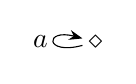
\begin{tikzpicture}
              \node (v1) at (1,0) {$\diamond$};
              \draw[loopstyle] (v1) to [loop left] node[midway, left, draw=none] {$a$} (v1);
            \end{tikzpicture}
    \end{center}
    in the extension $\QQ[\sqrt{-1}]/\QQ$ in the sense of Definition \ref{def:quiverrestriction}. This is the disconnected quiver 
    \begin{center}
            \hspace*{2em}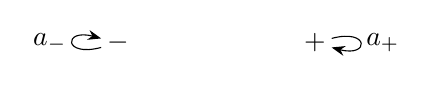
\begin{tikzpicture}
                \node (v1) at (-0.25,0) {$-$};
                \node (v2) at (2.25,0) {$+$};
                \draw[loopstyle] (v1) to [loop left] node[midway, left, draw=none] {$a_-$} (v1);
                \draw[loopstyle] (v2) to [loop right] node[midway, right, draw=none] {$a_+$} (v2);
            \end{tikzpicture}
    \end{center}
    endowed the following action of $G$, i.\,e.\ the non-trivial element $c\in G$ acts via:
    \[
    c\pm :=\mp,\quad c a_\pm:=\mp.
    \]
    The vertices $+$ and $-$ lie in the same orbit $\{+,-\}$ and $a_+$ and $a_-$ lie in one orbit $\{a_+,a_-\}$. Hence we have $I=\{+,-\}$. The stabilizers of vertices and edges are trivial in all cases, so that the associated \'etale $\QQ$-species is given by
    \begin{center}
            \hspace*{2em}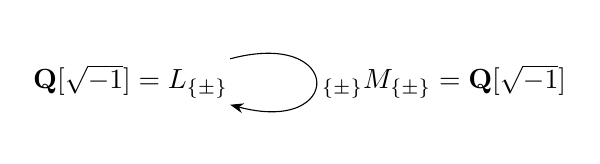
\begin{tikzpicture}
              \node (v1) at (1,0) {$\QQ[\sqrt{-1}]=L_{\{\pm\}}\quad$};
                \draw[loopstyle] (v1) to [loop right] node[midway, right, draw=none] {${}_{\{\pm\}}M_{\{\pm\}}=\QQ[\sqrt{-1}]$} (v1);
            \end{tikzpicture}
    \end{center}
    Here the $\QQ[\sqrt{-1}],\QQ[\sqrt{-1}]$-bimodule
    \[
    {}_{\{\pm\}}M_{\{\pm\}}=\QQ[\sqrt{-1}]
    \]
    carries the canonical bimodule structure given by left and right multiplication.
    \end{example}

    \begin{example}\label{ex:cyclic}
    We consider the cyclic quiver $Q_{\rm cyclic}$:
    \begin{center}
            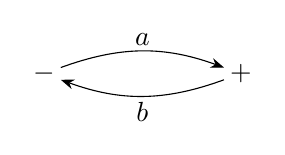
\begin{tikzpicture}
                \node (v1) at (-0.25,0) {$-$};
                \node (v2) at (2.25,0) {$+$};

                \draw[arr] (v1) to [bend left=20] node[midway, above, draw=none] {$a$} (v2);
                \draw[arr] (v2) to [bend left=20] node[midway, below, draw=none] {$b$} (v1);
            \end{tikzpicture}
    \end{center}
    and endow it with an action of by defining:
    \[
    c\pm :=\mp,\quad c a:=b,\quad cb:=a.
    \]
    Then $+$ and $-$ lie in the same orbit $\{+,-\}$ and $a$ and $b$ lie in one orbit $\{a,b\}$. Again we have $I=\{+,-\}$ and again the stabilizers of vertices and edges are trivial in all cases. However, in this case
    \[
    {}_{\{\pm\}}M_{\{\pm\}}=\QQ[\sqrt{-1}]\otimes_{\QQ[\sqrt{-1}],\tau}\QQ[\sqrt{-1}]=:\QQ[\sqrt{-1}]^{\rm twisted},
    \]
    is isomorphic to $\QQ[\sqrt{-1}]$ with a non-trivial bimodule structure: One of the two sides acts via a complex conjugate action, while the other side acts with the standard action.

    The associated \'etale $\QQ$-species is given by
    \begin{center}
            \hspace*{2em}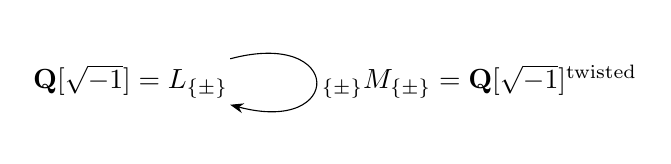
\begin{tikzpicture}
                \node (v1) at (1,0) {$\QQ[\sqrt{-1}]=L_{\{\pm\}}\quad$};
                \draw[loopstyle] (v1) to [loop right] node[midway, right, draw=none] {${}_{\{\pm\}}M_{\{\pm\}}=\QQ[\sqrt{-1}]^{\rm twisted}$} (v1);
            \end{tikzpicture}
    \end{center}
  \end{example}

  \begin{example}\label{ex:gelfand}
    We consider the Gelfand quiver $Q_{\rm Gelfand}$, which is the quiver with relation
    \begin{center}
    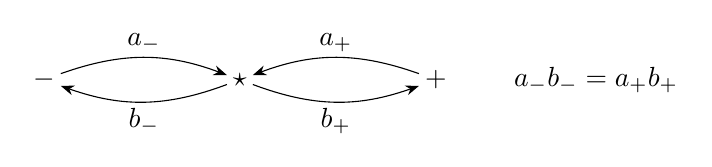
\begin{tikzpicture}[baseline=(current bounding box.center)]
    \node (A) {$-$};
    \node (B) [right=6em of A] {$\star$};
    \node (C) [right=6em of B] {$+$};
    \node (D) [right=2em of C] {$a_{-} b_{-} = a_{+} b_{+}$};
    \draw [arr, bend left=20] (A) to node [midway, above] {$a_{-}$} (B);
    \draw [arr, bend left=20] (B) to node [midway, below] {$b_{-}$} (A);
    \draw [revarr, bend left=20] (B) to node [midway, above] {$a_{+}$} (C);
    \draw [revarr, bend left=20] (C) to node [midway, below] {$b_{+}$} (B);
    \end{tikzpicture}
    \end{center}
    We define the $G$-action as:
    \[
    c\pm :=\mp,\quad c\star := \star,\quad c a_{\pm}:=a_{\mp},\quad cb_{\pm}:=b_{\mp}.
    \]
    This action of $c$ is compatible with the given relation $a_{-} b_{-} = a_{+} b_{+}$ and thus defines a $\QQ$-structure (or $\RR$-structure or $K$-structure) on the Gelfand quiver. Moreover, the relation is a consequence of $G$-equivariance and hence may be dropped when considering representations over $\QQ$ (resp.\ $\RR$ or $K$).

    Because of $G\pm=\{+,-\}$ and $G\star = \{\star\}$, the resulting \'etale $\QQ$-species has associated field extensions
    \begin{align*}
    L(\star)&=\QQ[\sqrt{-1}]^{G_\star}=\QQ[\sqrt{-1}]^{G}=\QQ,\\
    L(\pm)&=\QQ[\sqrt{-1}]^{G_{\pm}}=\QQ[\sqrt{-1}]^{\{\bf1\}}=\QQ[\sqrt{-1}].
    \end{align*}
    Likewise, for the two arrows $a_\pm$ we have
    \begin{align*}
    L(a_\pm)&=\QQ[\sqrt{-1}]^{G_{a_\pm}}=\QQ[\sqrt{-1}]^{\{\bf1\}}=\QQ[\sqrt{-1}],\\
    L(b_\pm)&=\QQ[\sqrt{-1}]^{G_{b_\pm}}=\QQ[\sqrt{-1}]^{\{\bf1\}}=\QQ[\sqrt{-1}].
    \end{align*}
    The index set is $I=\{\{\star\},\{+,-\}\}$. Therefore, the associated \'etale $\QQ$-species is
    \begin{center}
    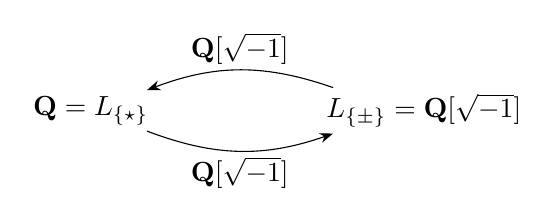
\begin{tikzpicture}[baseline=(current bounding box.center)]
    \node (Mstar) {$\QQ=L_{\{\star\}}$};
    \node (M+)    [right=4em of Mstar] {\quad\quad$L_{\{\pm\}}=\QQ[\sqrt{-1}]$};
    \draw [arr, bend right=20] (Mstar) to node [below] {$\QQ[\sqrt{-1}]$} (M+);
    \draw [arr, bend right=20] (M+) to node [above] {$\QQ[\sqrt{-1}]$} (Mstar);
    \end{tikzpicture}
    \end{center}
    Here the $\QQ,\QQ[\sqrt{-1}]$- and $\QQ[\sqrt{-1}],\QQ$-bimodules
    \[
      {}_{\{\star\}}M_{\{\pm\}}=\QQ[\sqrt{-1}],\quad
      {}_{\{\pm\}}M_{\{\star\}}=\QQ[\sqrt{-1}],
    \]
    carry the natural bimodule structures. The $c$-twisted structures would provide us with isomorphic $K$-species.

  To illustrate Theorem \ref{thm:KrationalquiveretaleKspeciesantiequivalence} in this case, observe that
  \begin{align*}
  \Hom_\QQ(L_{\{\star\}}\,\QQ[\sqrt{-1}])&=
  \Hom_\QQ(\QQ,\QQ[\sqrt{-1}])=\{\iota\colon\QQ\to\QQ[\sqrt{-1}]\},\\[0.5em]
  \Hom_\QQ(L_{\{\pm\}},\QQ[\sqrt{-1}])&=
  \Hom_\QQ(\QQ[\sqrt{-1}],\QQ[\sqrt{-1}])=G=\{{\bf1},c\},
  \end{align*}
  Hence, the set of vertices of $\Gamma_K(S(Q_{\rm Gelfand}))$ is
  \[
  V=\{\iota,{\bf1},c\}\;\cong\;\{\star,+,-\},
  \]
  and the edge set is given by
  \begin{align*}
  E&=
  \Hom_{\QQ}(L_{\{\star\}\to\{\pm\}},\QQ[\sqrt{-1}])\sqcup
  \Hom_{\QQ}(L_{\{\pm\}\to\{\star\}},\QQ[\sqrt{-1}])\\
  &=
  \Hom_{\QQ}(\QQ[\sqrt{-1}],\QQ[\sqrt{-1}])\sqcup
  \Hom_{\QQ}(\QQ[\sqrt{-1}],\QQ[\sqrt{-1}])\\
  &=G\sqcup G.
  \end{align*}
  The elements of $G\sqcup G$ give rise to the four directed edges of the Gelfand quiver. We obtain source and targets by precomposition with $\iota$ and $\sigma\in G$. Which composition is the source and which composition is the target depends on the direction of the arrow between $\{\star\}$ and $\{\pm\}$.
  \end{example}

  \subsection{Representations of \'etale $K$-species}

  \begin{definition}[Representation of a $K$-species]
  Let $S=(L_i, {}_iM_j)_{i,j\in I}$ be a $K$-species. A \emph{representation} of $S$ is a pair $(W, f)$ consisting of a collection $W = (W_i)_{i \in I}$ of finite-dimensional right $L_i$-vector spaces, and a collection $f = (f_{ij})_{i,j \in I}$ of $L_j$-linear maps
  \[
    f_{ij} \colon W_i \otimes_{L_i} {}_iM_j \to W_j.
  \]
  A \emph{morphism} $\psi \colon (W, f) \to (W', f')$ between two representations of $S$ is a collection of $L_i$-linear maps $\psi_i \colon W_i \to W'_i$ such that for all $i,j \in I$, the following diagram commutes:
  \begin{center}
  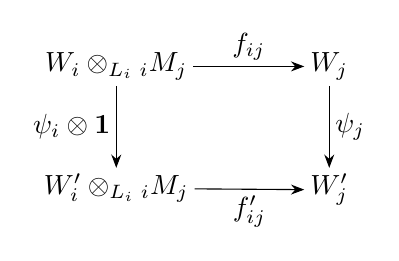
\begin{tikzpicture}[>=Stealth]
  \matrix (m) at (0,0) [matrix of math nodes, row sep=3em, column sep=4em]
  {
    W_i \otimes_{L_i} {}_iM_j & W_j \\
    W'_i \otimes_{L_i} {}_iM_j & W'_j \\
  };
  \path[-Stealth] (m-1-1) edge node[above] {$f_{ij}$} (m-1-2);
  \path[-Stealth] (m-1-1) edge node[left] {$\psi_i \otimes {\bf1}$} (m-2-1);
  \path[-Stealth] (m-1-2) edge node[right] {$\psi_j$} (m-2-2);
  \path[-Stealth] (m-2-1) edge node[below] {$f'_{ij}$} (m-2-2);
  \end{tikzpicture}
  \end{center}
  The category of finite-dimensional representations of $S$ is denoted by $\Rep(S)$.
  \end{definition}

  \begin{remark}
      Since the fields $L_i$ are commutative, we may identify left and right vector spaces, but we maintain the distinction for clarity in tensor products. We consider ${}_iM_j$ as left $L_i$ and as a right $L_j$-vector space.
  \end{remark}

  \begin{definition}[Base change for representations of \'etale $K$-species]
    Let $S=(L_i, {}_iM_j)_{i,j\in I}$ be a $K$-species and $W=(W_i,f_{ij})_{i,j\in I}$ a representation of $S$. Write $S\otimes_K N=(L_i',{}_iM_j')_{i,j\in I_N}$ for the base change of $S$ inside an extension $N/K$.
    \begin{itemize}
    \item[(i)] For any $i\in I$ and any $k\in J(i)\subseteq I_N$ put
      \[W_k':=W_i\otimes_{L_i}L_k'.\]
    \item[(ii)] For any $i,j\in I$ and any $k\in J(i)$ and $\ell\in J(\ell)$ put
      \[
      f_{k\ell}':=f_{ij}\otimes{\bf1}_{L_k'}\colon\;
      W_k'\otimes_{L_k'}{}_kM_\ell'=
      (W_i\otimes_{L_i}{}_iM_j)\otimes_{L_j} L_\ell'\to
      W_j\otimes_{L_j} L_\ell'=W_\ell'.
      \]
    \end{itemize}
    Then $W\otimes_KN:=(W_k',f_{k\ell}')_{k,\ell\in I_N}$ is a representation of $S\otimes_K N$ which we call the {\em base change} of $W$.
  \end{definition}

  \begin{remark}
    In light of Remark \ref{rmk:simplealgebraspecies} this notion of base change naturally extends to representations of $K$-species.
  \end{remark}

  \subsection{Categorical equivalence of representations}
  
  We construct a pair of quasi-inverse functors
  \[
  F \colon \Rep(\Gamma_K) \to \Rep(S(\Gamma_K))\quad\text{and}\quad H \colon \Rep(S(\Gamma_K)) \to \Rep(\Gamma_K).
  \]

  \paragraph{The functor $F \colon \Rep(\Gamma_K) \to \Rep(S(\Gamma_K))$.}
  Let
  \[
  M_K = ((M(v))_{v\in V}, (\varphi_{v,\sigma})_{v\in V,\sigma\in G}, (\phi_e)_{e\in E})
  \]
  be a $K$-rational representation of $\Gamma_K$. In order to define its image $F(M_K) = (W_i, f_{ij})_{i,j\in I}$ in $\Rep(S(\Gamma_K))$, we define the $L_i$-right vector spaces $W_i$ first. 

  \smallskip
  For each orbit $i \in I = G\backslash V$, we choose a representative $v_i \in i$ and define the $L_i$-vector space $W_i := M(v_i)^{G_{v_i}}$. The semi-linear action of $G_{v_i}$ on the $L$-vector space $M(v_i)$ makes the space of invariants $M(v_i)^{G_{v_i}}$ into a vector space over the fixed field $L_i = L^{G_{v_i}}$. By Galois descent (Thm.~\ref{thm:galoisdescent}), we have a canonical isomorphism of $L$-vector spaces
    \begin{equation}
      W_i\otimes_{L_i} L\cong M(v_i).
      \label{eq:WitoMvi}
    \end{equation}

    \smallskip
    The definition of the maps $f_{ij}$ is more involved. For each orbit $\varepsilon=Ge \in E/G$, we choose a representative $e_\varepsilon \in E$ and assume
    \[
    L_{\varepsilon}=L(e_\varepsilon).
    \]
    Write $i,j\in I$ for the $G$-orbits of $s(e_\varepsilon)$ and $t(e_\varepsilon)$ respectively. We fix $\sigma_\varepsilon,\tau_\varepsilon\in G$ with
    \begin{equation}
      s(e_\varepsilon)=\sigma_\varepsilon v_i\quad\text{and}\quad
      t(e_\varepsilon)=\tau_\varepsilon v_j.
      \label{eq:endsofedgetranslations}
    \end{equation}
    Then $L(e_\varepsilon)$ is an $L(v_i),L(v_j)$-bimodule via $(\sigma_\varepsilon,\tau_\varepsilon)$.

    \begin{proposition}
      For any right $L(e_\varepsilon)$-vector space $V$ we have a canonical isomorphism of $L$-vector spaces
    \begin{equation}
      V\otimes_{\tau_\varepsilon,L(v_j)}L
      =
      \prod_{\begin{subarray}c\eta G_{\tau_\varepsilon^{-1}e_\varepsilon}\in\\G_{v_j}/G_{\tau_\varepsilon^{-1}e_\varepsilon}\end{subarray}} V\otimes_{L(e_\varepsilon),\eta\tau_\varepsilon^{-1}}L.
      \label{eq:Leepsilondecomposition}
    \end{equation}
    On pure tensors, this isomorphism is given by
    \(
    v\otimes a\mapsto (v\otimes a)_{\eta\in G_{v_j}}.
    \)
    \end{proposition}

    \begin{proof}
    We have the canonical bimodule decomposition
    \begin{equation}
      L(e_\varepsilon)\otimes_{\tau_\varepsilon,L(v_j)}L
      =
      \prod_{\tau\colon L(\tau_\varepsilon^{-1}e_\varepsilon)\to L}
      L(e_\varepsilon)\otimes_{L(e_\varepsilon),\tau\tau_\varepsilon^{-1}}L,
      \label{eq:Leepsilondecompositionpre}
    \end{equation}
    where $\tau$ runs through all $L(v_j)$-linear embeddings (cf.\ \eqref{eq:endsofedgetranslations}).

    Writing $\iota_{\varepsilon}\colon L(\tau_\varepsilon^{-1}e_\varepsilon)\to L$ for the canonical inclusion corresponding to the inclusion $G_{\tau_\varepsilon^{-1}e_\varepsilon}\to G$, each $L(v_j)$-linear $\tau$ is of the form
    \[
    \tau=\eta\iota_{\varepsilon},\quad\text{for a unique coset }\eta G_{\tau_\varepsilon^{-1}e_\varepsilon} \in G_{v_j}/G_{\tau_\varepsilon^{-1}e_\varepsilon}.
    \]
    Hence \eqref{eq:Leepsilondecompositionpre} implies that for any right $L(e_\varepsilon)$-vector space $V$ we have \eqref{eq:Leepsilondecomposition} and the map has the given description.
    \end{proof}

    \begin{proposition}\label{prop:WiiMjLpre}
      We have a canonical isomorphism of $L$-vector spaces
    \begin{equation}
    W_i \otimes_{L_i} {}_iM_j\otimes_{L_j}L=
    \bigoplus_{\varepsilon\in G\backslash E_{ij}}
    \prod_{\eta}
    M(v_i)^{G_{v_i}} \otimes_{L(v_i),\eta\tau_\varepsilon^{-1}\sigma_\varepsilon}L,
    \label{eq:WiiMjLpre}
    \end{equation}
    where $\eta$ runs through a system of representatives for $G_{v_j}/G_{\tau_\varepsilon^{-1}e_\varepsilon}$.
    \end{proposition}

    \begin{proof}
    Recalling the definition of ${}_iM_j$ we rewrite
    \[
    W_i \otimes_{L_i} {}_iM_j\otimes_{L_j}L=
    \bigoplus_{\varepsilon\in G\backslash E_{ij}}
    M(v_i)^{G_{v_i}} \otimes_{L(v_i),\sigma_\varepsilon} L(e_\varepsilon)\otimes_{\tau_\varepsilon,L(v_j)}L.
    \]
    In light of the decomposition \eqref{eq:Leepsilondecomposition}, identity \eqref{eq:WiiMjLpre} follows.
    \end{proof}


    \begin{proposition}\label{prop:generalextensionofscalars}
      For any $v\in V$ and any $\sigma\in G$ the given semilinar map $\varphi_{v,\sigma}\colon M(v)\to M(\sigma v)$ induces a map $M(v)^{G_{v}}\to M(\sigma v)$ which extends to a unique $L$-linear map
    \begin{equation}
      M(v)^{G_{v}}\otimes_{L(v),\sigma}L\to M(\sigma v),\;m\otimes a\mapsto \varphi_{v,\sigma}(m)\cdot a,
      \label{eq:generalextensionisomorphism}
    \end{equation}
    which is an isomorphism of $L$-vector spaces. Moreover, by the same universal property, we have for any $\tau\in G$ a commutative square
    \begin{equation}
      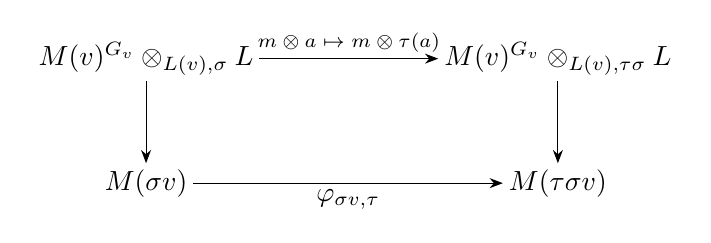
\begin{tikzpicture}[>=Stealth]
        \matrix (m) at (0,0) [matrix of math nodes, row sep=3em, column sep=6.5em]
                {
                  M(v)^{G_{v}}\otimes_{L(v),\sigma}L & M(v)^{G_{v}}\otimes_{L(v),\tau\sigma}L \\
                  M(\sigma v) & M(\tau\sigma v) \\
                };
                \path[-Stealth] (m-1-1) edge node[font=\scriptsize, above] {$m\otimes a\mapsto m\otimes\tau(a)$} (m-1-2);
                \path[-Stealth] (m-1-1) edge (m-2-1);
                \path[-Stealth] (m-1-2) edge (m-2-2);
                \path[-Stealth] (m-2-1) edge node[below] {$\varphi_{\sigma v,\tau}$} (m-2-2);
      \end{tikzpicture}
      \label{eq:semi-linearsquare}
    \end{equation}
    \end{proposition}

    \begin{proof}
      Existence and uniqueness of \eqref{eq:generalextensionisomorphism} follows by the universalm property of the left hand side. Galois descent shows that \eqref{eq:generalextensionisomorphism} is an isomorphism of $L$-vector spaces. The commutativity of \eqref{eq:semi-linearsquare} follows by the universal property of $M(v)^{G_{v}}\otimes_{L(v),\sigma}L$.
    \end{proof}

    \begin{corollary}\label{cor:WiiMjL}
    We have canonical $L$-linear isomorphisms
    \begin{equation}
      \psi_{i,j,\varepsilon,\eta}\colon M(v_i)^{G_{v_i}} \otimes_{L(v_i),\eta\tau_\varepsilon^{-1}\sigma_\varepsilon}L\to M(\eta\tau_\varepsilon^{-1}\sigma_\varepsilon).
      \label{eq:Llinearisos}
    \end{equation}
    In particular, we have for all $i,j\in I$ a canonical isomorphism
    \begin{equation}
    W_i \otimes_{L_i} {}_iM_j\otimes_{L_j}L=
    \bigoplus_{\varepsilon\in G\backslash E_{ij}}
    \prod_{\eta}
    M(\eta\tau_\varepsilon^{-1}\sigma_\varepsilon v_i).
    \label{eq:WiiMjL}
    \end{equation}
    \end{corollary}

    \begin{proof}
       We apply Proposition \ref{prop:generalextensionofscalars} to each summand on the right hand side of \eqref{eq:WiiMjLpre}.
    \end{proof}
    
    The identification \eqref{eq:WiiMjL} gives rise to the following $L(v_j)$-rational structure on $W_i \otimes_{L_i} {}_iM_j\otimes_{L_j}L$. For any $\sigma\in \Gal(L/L(v_j))=G_{v_j}$ we consider the map
    \begin{align*}
    \Theta_{ij}(\sigma)\colon\;
    \bigoplus_{\varepsilon\in G\backslash E_{ij}}
    \prod_{\eta\in G_{v_j}}
    M(\eta\tau_\varepsilon^{-1}\sigma_\varepsilon v_i)
    &\to
    \bigoplus_{\varepsilon\in G\backslash E_{ij}}
    \prod_{\eta\in G_{v_j}}
    M(\eta\tau_\varepsilon^{-1}\sigma_\varepsilon v_i)\\
    (m_{\varepsilon,\eta})_{\varepsilon,\eta}&\mapsto
    \left(\varphi_{\sigma^{-1}\eta\tau_\varepsilon^{-1}\sigma_\varepsilon v_i,\sigma}(m_{\varepsilon,\sigma^{-1}\eta})\right)_{\varepsilon,\eta}.
    \end{align*}
    This map is clearly $\sigma$-linear and satisfies the cocycle condition
    \[
    \forall\sigma,\tau\in G_{v_j}:\quad\Theta_{ij}(\sigma)\circ\Theta_{ij}(\tau)=\Theta_{ij}(\sigma\tau).
    \]
    Hence we obtain an $L(v_j)$-rational structure on $W_i \otimes_{L_i} {}_iM_j\otimes_{L_j}L$ as claimed.

    \begin{proposition}\label{prop:rationalstructures}
      The $L(v_j)$-rational structure $\Theta_{ij}$ on $W_i \otimes_{L_i} {}_iM_j\otimes_{L_j}L$ agrees with the canonical $L(v_j)$-rational structure
      \[
      W_i \otimes_{L_i} {}_iM_j\;\subseteq\; W_i \otimes_{L_i} {}_iM_j\otimes_{L_j}L.
      \]
    \end{proposition}

    \begin{proof}
      Note that the canonical $L_j$-rational structure on $W_i \otimes_{L_i} {}_iM_j\otimes_{L_j}L$ corresponds to the semi-linear automorphisms
      \[w\otimes m\otimes a\mapsto w\otimes m\otimes\sigma a,\]
      for $\sigma\in\Gal(L/L(v_j))$.

      In order to see that both rational structures agree, we observe that for any $\sigma\in\Gal(L/L(v_j))$ we consider the semi-linear automorphism
    \[
    {\bf1}_{V}\otimes \sigma\colon V\otimes_{\tau_\varepsilon,L(v_j)}L\to V\otimes_{\tau_\varepsilon,L(v_j)}L,\;v\otimes a\mapsto v\otimes\sigma a.
    \]
    In light of the explicit description of the right $L$-vector space isomorphism \eqref{eq:WiiMjLpre}, we have the commutative square
    \begin{center}
      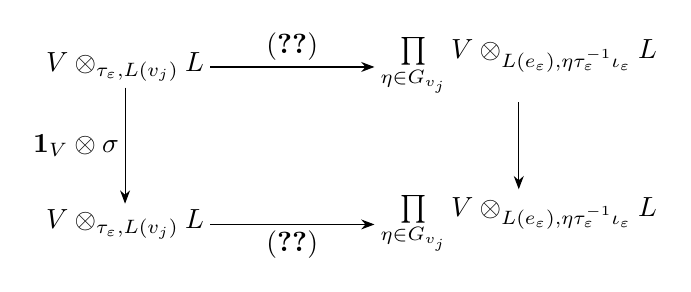
\begin{tikzpicture}[>=Stealth]
        \node (N1) at (0,0) {$V\otimes_{\tau_\varepsilon,L(v_j)}L$};
        \node (N2) at (5,0) {$\prod\limits_{\eta\in G_{v_j}} V\otimes_{L(e_\varepsilon),\eta\tau_\varepsilon^{-1}\iota_\varepsilon}L$};
        \node (N3) at (0,-2) {$V\otimes_{\tau_\varepsilon,L(v_j)}L$};
        \node (N4) at (5,-2) {$\prod\limits_{\eta\in G_{v_j}} V\otimes_{L(e_\varepsilon),\eta\tau_\varepsilon^{-1}\iota_\varepsilon}L$};
        % Top horizontal arrow
        \draw[-Stealth] (N1.east) -- (N2.west) node[midway,above] {\eqref{eq:WiiMjLpre}};
        % Left vertical arrow
        \draw[-Stealth] (N1.south) -- (N3.north) node[midway,left] {$\mathbf{1}_{V}\otimes \sigma$};
        % Right vertical arrow (no label in your original diagram)
        \draw[-Stealth] (N2.south) -- (N4.north);
        % Bottom horizontal arrow
        \draw[-Stealth] (N3.east) -- (N4.west) node[midway,below] {\eqref{eq:WiiMjLpre}};
      \end{tikzpicture}
    \end{center}
    where the right vertical map is given by
    \begin{equation}
      (m_\eta\otimes a_\eta)_{\eta\in G_{v_j}}\mapsto (m_{\sigma^{-1}\eta}\otimes \sigma a_{\sigma^{-1}\eta} )_{\eta\in G_{v_j}}
      \label{eq:explicitdecompositiontwisting}
    \end{equation}
    This map descends mutatis mutandis to a $\sigma$-linear automorphism of the right hand side of \eqref{eq:WiiMjLpre}. By the commutativity of \eqref{eq:semi-linearsquare}, this shows that the corresponding map on the right hand side of \eqref{eq:WiiMjL} is explicitly given by
    \[
    (m_{\varepsilon,\eta})_{\varepsilon,\eta}\mapsto
    \left(\varphi_{\sigma^{-1}\eta\tau_\varepsilon^{-1}\sigma_\varepsilon v_i,\sigma}(m_{\varepsilon,\sigma^{-1}\eta})\right)_{\varepsilon,\eta},
    \]
    which agrees with the Definition of $\Theta_{ij}(\sigma)$. This shows the claim.
    \end{proof}
    
    To define the maps
    \[f_{ij} \colon W_i \otimes_{L_i} {}_iM_j \to W_j\]
    we first base change to $L$ on the domain and codomain to define
    \[f_{ij}\otimes{\bf1}_L \colon W_i \otimes_{L_i} {}_iM_j\otimes_{L_j}L \to W_j\otimes_{L_j}L\]
    using \eqref{eq:WiiMjL}. Then we will define $f_{ij}$ as a suitable Galois descent of the yet-to-be-defined map $f_{ij}\otimes{\bf1}_L$.
    
    As for the definition of $f_{ij}\otimes{\bf1}_L$, we put
    \begin{align*}
    \Phi_{ij}\colon
    \bigoplus_{\varepsilon\in G\backslash E_{ij}}
    \prod_{\eta}
    M(v_i)^{G_{v_i}} \otimes_{L(v_i),\eta\tau_\varepsilon^{-1}\sigma_\varepsilon}L
    &\to
    M(v_j)=M(v_j)^{G_{v_j}}\otimes_{L(v_j)}L,\\
    (m_{\varepsilon,\eta}\otimes a_{\varepsilon,\eta})_{\varepsilon,\eta}&\mapsto
    \sum_{\varepsilon,\eta}
    %\varphi_{\eta\tau_\varepsilon^{-1}\sigma_\varepsilon v_j,\sigma_\varepsilon^{-1}\tau_\varepsilon\eta^{-1}}(
    \varphi_{t(e_\varepsilon),\eta\tau_\varepsilon^{-1}}\phi_{e_\varepsilon}\varphi_{e_i,\sigma_\varepsilon}(m_{\varepsilon,\eta})\cdot a_{\varepsilon,\eta}.
    \end{align*}

    \begin{proposition}
      $\Phi_{ij}$ descends to an $L_j$-linear map
      \[
      f_{ij}\colon W_i \otimes_{L_i} {}_iM_j \to W_j.
      \]
    \end{proposition}

    \begin{proof}
      We show that $\Phi_{ij}$ is $G_{v_j}$-equivariant. For a arbitrary element $(m_{\varepsilon,\eta}\otimes a_{\varepsilon,\eta})_{\varepsilon,\eta}$ we compute:
      \begin{align*}
      \Phi_{ij}\left(\Theta_{ij}(\sigma)((m_{\varepsilon,\eta}\otimes a_{\varepsilon,\eta})_{\varepsilon,\eta})\right)
      &=
      \Phi_{ij}\left((m_{\varepsilon,\sigma^{-1}\eta}\otimes \sigma a_{\varepsilon,\sigma^{-1}\eta} )_{\varepsilon,\eta}\right)\\
      &=
      \sum_{\varepsilon,\eta}
      \varphi_{t(e_\varepsilon),\eta\tau_\varepsilon^{-1}}\phi_{e_\varepsilon}\varphi_{e_i,\sigma_\varepsilon}(m_{\varepsilon,\sigma^{-1}\eta})\cdot \sigma a_{\varepsilon,\sigma^{-1}\eta}\\
      &=
      \sum_{\varepsilon,\eta}
      \varphi_{t(e_\varepsilon),\sigma\eta\tau_\varepsilon^{-1}}\phi_{e_\varepsilon}\varphi_{e_i,\sigma_\varepsilon}(m_{\varepsilon,\eta})\cdot \sigma a_{\varepsilon,\eta}\\
      &=
      \varphi_{t(e_j),\sigma}
      \left(
      \sum_{\varepsilon,\eta}
      \varphi_{t(e_\varepsilon),\eta\tau_\varepsilon^{-1}}\phi_{e_\varepsilon}\varphi_{e_i,\sigma_\varepsilon}(m_{\varepsilon,\eta})\cdot a_{\varepsilon,\eta}
      \right)\\
      &=
      \varphi_{t(e_j),\sigma}
      \left(
      \Phi_{ij}\left((m_{\varepsilon,\eta}\otimes a_{\varepsilon,\eta})_{\varepsilon,\eta}\right)
      \right).
      \end{align*}
      where we invoked \eqref{eq:explicitdecompositiontwisting} for the first identity. This proves the Galois-equivariance with respect to the rational structure defined by $\Theta_{ij}$. By Proposition \ref{prop:rationalstructures}, this rational structure agrees with the canonical rational structure. Therefore, $\Phi_{ij}$ descends via Galois descent to an $L_j$-linear map $f_{ij}$ as claimed.
    \end{proof}

    \begin{proposition}
      For any morphism $\psi \colon M_K \to N_K$ in $\Rep(\Gamma_K)$ the collection of $L$-linear maps $\phi_v \colon M(v) \to N(v)$ for $v\in V$ induces for any $i\in I=G\backslash V$ a canonical $L_i$-linear map
      \[
      \psi_{i}\colon M(v)^{G_{v_i}}\to N(v)^{G_{v_i}}.
      \]
      The collection $(\psi_i)_{i\in I}$ defines a morphism $S(M_K)\to S(N_K)$ of $K$-species representations.
      \end{proposition}

      \begin{proof}
        We observe that for any $i\in I$ condition \eqref{eq:koecheractiononrephom} implies that $\psi_{v_i}$ is $G_{v_i}$-equivariant and hence descends to an $L^{G_{v_i}}$-linear map as claimed.
        
      Assume that
      \[
      M_K=((V_v)_{v\in V},(\phi_e)_{e\in E})\quad\text{and}\quad
      N_K=((V_v')_{v\in V},(\phi_e')_{e\in E})
      \]
      Then an elementary calculation shows that the $L$-linear maps $\Phi_{ij}$ underlying the defin ition of $f_{ij}$ commute with the collection of the maps $\psi_{v_i}$ by \eqref{eq:koecheractiononrep}. By Galois descent, this implies that the maps $\psi_{i}$ for $i\in I$ define a $K$-species homomorphism as claimed.      
      \end{proof}

      \begin{theorem}\label{thm:quiveretalespeciesrepresentations}
        The maps
        \begin{equation}
        S\colon M_K=((V_v)_{v\in V},(\varphi_{v,\sigma})_{v\in V,\sigma\in G},(\phi_e)_{e\in E})\;\mapsto\;((V_{v_i}^{G_{v_i}})_{i\in I},(f_{ij})_{i,j\in I}),
        \end{equation}
        and
        \begin{equation}
        S\colon \left((\psi_v)_{v\in V}\colon M_K\to N_K\right)\;\mapsto\;(\psi_i)_{i\in I}
        \end{equation}
        defines a functor $\Rep(\Gamma_K)\to\Rep(S(\Gamma_K))$.
      \end{theorem}

      \begin{proof}
        By our previous considerations both maps are well defined. The verification of the functor properties is straightforward.
      \end{proof}


  \paragraph{The functor $H \colon \Rep(S(\Gamma_K)) \to \Rep(\Gamma_K)$.}
  Let
  \[
  (W_{i}, f_{ij})_{i,j\in I}
  \]
  be a representation of $S(\Gamma_K)$. We are going to define a representation of the $K$-rational quiver $\Gamma_K$
  \[
  H((W_i, f_{ij})) = ((M(v))_{v\in V}, (\varphi_{v,\sigma})_{v\in V,\sigma\in G},(\phi_e)_{e\in E})
  \]
  as follows.

  We fix for every $i\in I$ a $K$-rational structure
  \begin{equation}
    W_{i,K}\subseteq W_i,
    \label{eq:KrationalWi}
  \end{equation}
  Then for each vertex $v \in V$, we consider its orbit $i=Gv$, which by our previous choices in the previous section above, agrees with $Gv_{i}$. With these choices we put
  \begin{equation}
    M(v) := W_{i,K}\otimes_{K}L.
    \label{eq:MvforWi}
  \end{equation}
  Then we have for every $\sigma\in G$ a canonical $\sigma$-linear isomorphism
  \begin{equation}
    \varphi_{v,\sigma}\colon M(v)\to M(\sigma v),\quad w\otimes a\mapsto w\otimes \sigma a.
    \label{eq:varphi2}
  \end{equation}
  These isomorphisms satisfy the cocycle condition \eqref{eq:semi-linearactiononrep}.

  In order to define for every $e\in E$ an $L$-linear map $\phi_e\colon V(s(t))\to V(t(e))$ satisfying \eqref{eq:koecheractiononrep}, we proceed as follows. We first consider the following analogue of Corollary \ref{cor:WiiMjL}.

  \begin{proposition}
    For every $i,j\in I$ and every $\varepsilon\in E_{ij}$ recall the chosen representative $e_\varepsilon\in\varepsilon$ and let $\sigma_\varepsilon,\tau_\varepsilon\in G$ be as in \eqref{eq:endsofedgetranslations}. Then in light of definition \eqref{eq:MvforWi}, we have a canonical isomorphism
    \begin{equation}
    W_i \otimes_{L_i} {}_iM_j\otimes_{L_j}L=
    \bigoplus_{\varepsilon\in G\backslash E_{ij}}
    \bigoplus_{\eta}
    M(\eta\tau_\varepsilon^{-1}\sigma_\varepsilon v_i),
    \label{eq:WiiMjL2}
    \end{equation}
    where $\eta$ runs through a system of representatives for $G_{v_j}/G_{\tau_\varepsilon^{-1}e_\varepsilon}$.
  \end{proposition}

  \begin{proof}
    Observe first that we have an isomorphism
    \[
    W_{i,K}\otimes_K L_i\to W_i.
    \]
    Recalling our definition ${}_iM_j=L(e_\varepsilon)$ gives us
    \begin{align*}
      W_i \otimes_{L_i} {}_iM_j\otimes_{L_j}L
      &=\bigoplus_{\varepsilon\in G\backslash E_{ij}}W_{i}\otimes_{L(v_i),\sigma_\varepsilon} L(e_\varepsilon)\otimes_{\tau_\varepsilon,L(v_j)}L\\
      &=\bigoplus_{\varepsilon\in G\backslash E_{ij}}W_{i}\otimes_{L(v_i),\sigma_\varepsilon} \prod_{\eta}L(e_\varepsilon)\otimes_{L(e_\varepsilon),\eta\tau_\varepsilon^{-1}}L&\text{(by \eqref{eq:Leepsilondecomposition})}\\
      &=\bigoplus_{\varepsilon\in G\backslash E_{ij}}W_{i}\otimes_{L(v_i)} \prod_{\eta}L(v_i)\otimes_{L(v_i),\eta\tau_\varepsilon^{-1}\sigma_\varepsilon}L,
    \end{align*}
    where $\eta$ runs through a system of representatives for $G_{v_j}/G_{\tau_\varepsilon^{-1}e_\varepsilon}$ as before. By our choice of $K$-rational stucture, this agrees with
    \[
    W_{i,K}\otimes_K L_{v_i}\otimes_{L(v_i)} \prod_{\tau}L(v_i)\otimes_{L(v_i),\eta\tau_\varepsilon^{-1}\sigma_\varepsilon}L=
    \bigoplus_\eta W_{i,K}\otimes_K L(v_i)\otimes_{L(v_i),\eta\tau_\varepsilon^{-1}\sigma_\varepsilon}L,
    \]
    where we identified the finite direct product with a finite direct sum. Now the $\eta$-th direct summand on the right hand side is canonically isomorphic to $M(\eta\tau_\varepsilon^{-1}\sigma_\varepsilon v_i)$ via \eqref{eq:varphi2}. This proves the claim.
  \end{proof}

  For every $i,j\in I$ and every $e\in E_{ij}$ let $\sigma_e\in G$ be such that $\sigma_e e_{\varepsilon(e)}=e$ for $\varepsilon(e)=Ge$. Note that
  \[
  \sigma_e\tau_{\varepsilon(e)} v_j=
  \sigma_e t(e_{\varepsilon(e)})=
  t(\sigma_e e_{\varepsilon(e)})=
  t(e).
  \]
  Then we define $\phi_{e}\colon M(s(e))\to M(t(e))$ via \eqref{eq:WiiMjL2} as the composition
  \begin{align*}
      M(s(e))&= M(\sigma_e s(e_{\varepsilon(e)}))\\
      &=M(\sigma_e \sigma_{\varepsilon(e)} v_i)\\
      &\to M(\tau_{\varepsilon(e)}^{-1}\sigma_{\varepsilon(e)} v_i)&\text{(via $\varphi_{\sigma_e\sigma_{\varepsilon(e)}v_i,\tau_{\varepsilon(e)}^{-1}\sigma_e^{-1}}$)}\\
      &\to  \bigoplus_{\varepsilon\in G\backslash E_{ij}}
    \bigoplus_{\eta}
    M(\eta\tau_\varepsilon^{-1}\sigma_\varepsilon v_i)\\
    &=W_i \otimes_{L_i} {}_iM_j\otimes_{L_j}L\\
    &\to W_j \otimes_{L_j} L&\text{(via $f_{ij}\otimes{\bf1}_L$)}\\
    &\to M(t(e)) & \text{(via $\varphi_{v_j,\sigma_e\tau_{\varepsilon(e)}}$)}
  \end{align*}
  Note that this composition is $L$-linear by definition.
  \begin{proposition}
    For all $\sigma\in G$ and all $e\in E$ the $L$-linear map $\phi_e$ satisfies \eqref{eq:koecheractiononrep}.
  \end{proposition}

  \begin{proof}
    Let $i,j\in I$, $e\in E_{ij}$ and $\sigma\in G$. Then
    %\begin{equation}
    %  \sigma\sigma_e e_{\varepsilon(e)}=\sigma e=\sigma_{\sigma e} e_{\varepsilon(\sigma e)},
      %\quad\Rightarrow\quad
    %\sigma_{\sigma e}^{-1}\sigma\sigma_e e_{\varepsilon(e)}= e_{\varepsilon(\sigma e)}.
    %\label{eq:esigmae}
    %\end{equation}
    %and
    \begin{align*}
      \tau_{\varepsilon(\sigma e)}^{-1}\sigma_{\sigma e}^{-1}\sigma\sigma_e\tau_{\varepsilon(e)}v_j
      &=
      \tau_{\varepsilon(\sigma e)}^{-1}\sigma_{\sigma e}^{-1}\sigma\sigma_et(e_{\varepsilon(e)})\\
      &=
      \tau_{\varepsilon(\sigma e)}^{-1}t(\sigma_{\sigma e}^{-1}\sigma\sigma_ee_{\varepsilon(e)})\\
      &=
      \tau_{\varepsilon(\sigma e)}^{-1}t(\sigma_{\sigma e}^{-1}\sigma e)\\
      &=
      \tau_{\varepsilon(\sigma e)}^{-1}t(e_{\varepsilon(\sigma e)})\\
      &=
      v_j.
    \end{align*}
    Therefore,
    \[
          \eta_{e,\sigma}:=\tau_{\varepsilon(\sigma e)}^{-1}\sigma_{\sigma e}^{-1}\sigma\sigma_e\tau_{\varepsilon(e)}\in G_{v_j}.
    \]
    Now consider the square
    \begin{center}
    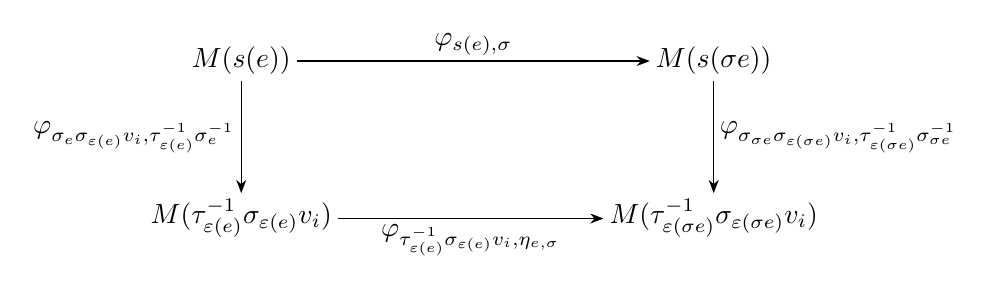
\begin{tikzpicture}[>=Stealth]
    \node (A) at (0,0) {$M(s(e))$};
    \node (B) at (6,0) {$M(s(\sigma e))$};
    \node (C) at (0,-2) {$M(\tau_{\varepsilon(e)}^{-1}\sigma_{\varepsilon(e)} v_i)$};
    \node (D) at (6,-2) {$M(\tau_{\varepsilon(\sigma e)}^{-1}\sigma_{\varepsilon(\sigma e)} v_i)$};

    \draw[->] (A) -- (B) node[midway, above] {$\varphi_{s(e),\sigma}$};
    \draw[->] (A) -- (C) node[midway, left] {$\varphi_{\sigma_e\sigma_{\varepsilon(e)}v_i,\tau_{\varepsilon(e)}^{-1}\sigma_e^{-1}}$};
    \draw[->] (B) -- (D) node[midway, right] {$\varphi_{\sigma_{\sigma e}\sigma_{\varepsilon(\sigma e)}v_i,\tau_{\varepsilon(\sigma e)}^{-1}\sigma_{\sigma e}^{-1}}$};
    \draw[->] (C) -- (D) node[midway, below] {$\varphi_{\tau_{\varepsilon( e)}^{-1}\sigma_{\varepsilon( e)}v_i,\eta_{e,\sigma}}$};
    \end{tikzpicture}
    \end{center}
    To verify its commutativity, we compute with \eqref{eq:semi-linearactiononrep}:
    \begin{align*}
      \varphi_{\tau_{\varepsilon( e)}^{-1}\sigma_{\varepsilon( e)}v_i,\eta_{e,\sigma}}
      \circ
      \varphi_{s(e),\tau_{\varepsilon(e)}^{-1}\sigma_e^{-1}}
      &=
      \varphi_{s(e),\eta_{e,\sigma}\tau_{\varepsilon(e)}^{-1}\sigma_e^{-1}}\\
      &=
      \varphi_{s(e),\tau_{\varepsilon(\sigma e)}^{-1}\sigma_{\sigma e}^{-1}\sigma\sigma_e\sigma_e^{-1}}\\
      &=
      \varphi_{s(e),\tau_{\varepsilon(\sigma e)}^{-1}\sigma_{\sigma e}^{-1}\sigma}\\
      &=
      \varphi_{\sigma_{\sigma e}\sigma_{\varepsilon(\sigma e)}v_i,\tau_{\varepsilon(\sigma e)}^{-1}\sigma_{\sigma e}^{-1}}
      \circ
      \varphi_{s(e),\sigma}.
    \end{align*}
    %Multiplication of $\eta$ with $\eta_{e,\sigma}$ permutes the direct summands in the relevant decomposition \eqref{eq:WiiMjL2} and therefore
    $\bigoplus\limits_\eta\varphi_{\bullet,\eta_{e,\sigma}}$ induces a canonical $\eta_{e,\sigma}$-linear isomorphism
    \[
    \bigoplus_{\eta}
    M(\eta\tau_{\varepsilon(e)}^{-1}\sigma_{\varepsilon(e)} v_i)
    \to
    \bigoplus_{\eta}
    M(\eta_{e,\sigma}\eta\eta_{e,\sigma}^{-1}\tau_{\varepsilon(\sigma e)}^{-1}\sigma_{\varepsilon(\sigma e)} v_i)
    =
    \bigoplus_{\eta}
    M(\eta\tau_{\varepsilon(\sigma e)}^{-1}\sigma_{\varepsilon(\sigma e)} v_i),
    \]
    which together with the canonical inclusions for the $\eta={\bf1}$-summands induces a commutative square. Adding a further layer of identifications, we obtain a commutative square
    \begin{center}
    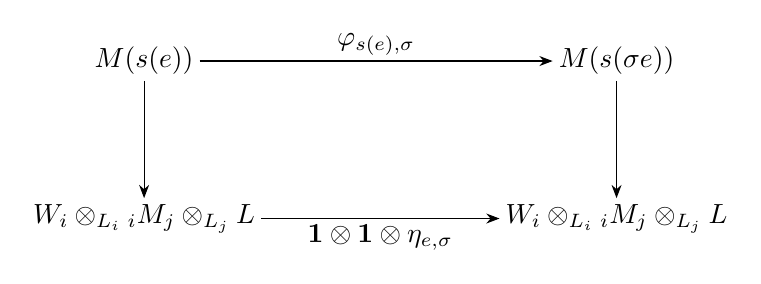
\begin{tikzpicture}[>=Stealth]
    \node (A) at (0,0) {$M(s(e))$};
    \node (B) at (6,0) {$M(s(\sigma e))$};
    \node (C) at (0,-2) {$W_i\otimes_{L_i}{}_iM_j\otimes_{L_j} L$};
    \node (D) at (6,-2) {$W_i\otimes_{L_i}{}_iM_j\otimes_{L_j} L$};

    \draw[->] (A) -- (B) node[midway, above] {$\varphi_{s(e),\sigma}$};
    \draw[->] (A) -- (C) node[midway, left] {};
    \draw[->] (B) -- (D) node[midway, right] {};
    \draw[->] (C) -- (D) node[midway, below] {${\bf1}\otimes{\bf1}\otimes\eta_{e,\sigma}$};
    \end{tikzpicture}
    \end{center}
    To conclude the proof, consider the diagram
    \begin{center}
    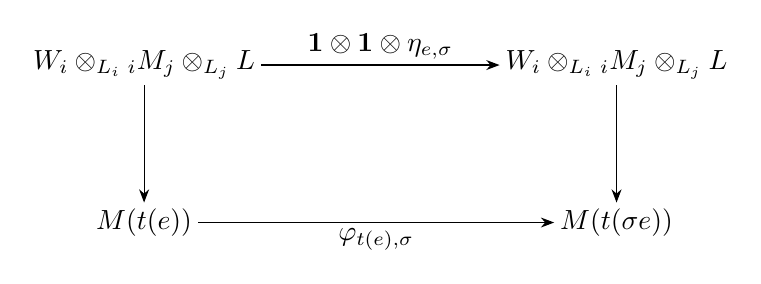
\begin{tikzpicture}[>=Stealth]
    \node (A) at (0,0) {$W_i\otimes_{L_i}{}_iM_j\otimes_{L_j} L$};
    \node (B) at (6,0) {$W_i\otimes_{L_i}{}_iM_j\otimes_{L_j} L$};
    \node (C) at (0,-2) {$M(t(e))$};
    \node (D) at (6,-2) {$M(t(\sigma e))$};

    \draw[->] (A) -- (B) node[midway, above] {${\bf1}\otimes{\bf1}\otimes\eta_{e,\sigma}$};
    \draw[->] (A) -- (C) node[midway, left] {};
    \draw[->] (B) -- (D) node[midway, right] {};
    \draw[->] (C) -- (D) node[midway, below] {$\varphi_{t(e),\sigma}$};
    \end{tikzpicture}
    \end{center}
    which commutes due to the definition of $M(-)$ via \eqref{eq:MvforWi} and the definition of $\varphi_{t(e),\sigma}$ via \eqref{eq:varphi2}, taking the vertical identifications via $\varphi_{v_j,\sigma_e\tau_{\varepsilon(e)}}$ and $\varphi_{v_j,\sigma_{\sigma e}\tau_{\varepsilon(\sigma e)}}$ into account.
  \end{proof}
  This defines the functor $H$ on objects. A morphism in $\Rep(S(\Gamma_K))$ naturally induces a morphism in $\Rep(\Gamma_K)$ in light of the definition of $M(v)$ via \eqref{eq:MvforWi}, making $H$ a functor.

  \begin{theorem}\label{thm:species_equivalence}
  Let $\Gamma_K$ be a $K$-rational quiver. The category $\Rep(\Gamma_K)$ of finite-dimensional $K$-rational representations of $\Gamma_K$ is equivalent to the category $\Rep(S(\Gamma_K))$ of finite-dimensional representations of its associated $K$-species $S(\Gamma_K)$.
  \end{theorem}

  \begin{proof}
  The constructions are such that they are mutually inverse up to natural isomorphism. For a species representation $(W_i, f_{ij})$, applying $H$ gives a rational quiver representation $M_K$. Applying $F$ to $M_K$ gives back spaces $M(v_i)^{G_{v_i}} = (W_i\otimes_{L_i}L)^{G_{v_i}} \cong W_i$, and the maps are likewise recovered.
  
  Conversely, starting with $M_K$, applying $F$ and then $H$ gives the representation with spaces $M(v_i)^{G_{v_i}}\otimes_{L_i}L$, which are naturally isomorphic to $M(v_i)$ by Galois descent. The maps are also recovered through this process.

  A straihgtforward verification considering morphisms, shows that $F \circ H \cong \mathrm{Id}_{\Rep(S(\Gamma_K))}$ and $H \circ F \cong \mathrm{Id}_{\Rep(\Gamma_K)}$.
  \end{proof}

  \begin{remark}
    Given the base change formalism for $K$-rational quivers, $K$-species and their associated representations, it is easy to verify that the categorical equivalences for varying $K$ define an equivalence of stacks in the \'etale topology on $K$.
  \end{remark}

\section{Rational Harish-Chandra modules}\label{sec:HC}

\subsection{Rational Harish-Chandra modules}

  We understand rational $(\mathfrak{g}, K)$-modules as in \cite{Januszewski18}. Specifically, a \emph{pair} over a field $k$ of characteristic 0 consists of a $k$-Lie algebra $\mathfrak{a}_k$ and a linear algebraic group $B_k$ over $k$, whose identity component $B^\circ$ is reductive. Furthermore, $\mathfrak{b}_k = \Lie_k(B_k) \subseteq \mathfrak{a}_k$, and there is a $k$-rational action of $B_k$ on $\mathfrak{a}_k$ that extends the natural action on $\mathfrak{b}_k$. An $(\mathfrak{a}_k, B_k)$-module over $k$ is a $k$-vector space that is a colimit of rational $B_k$-representations and is endowed with a $k$-linear $\mathfrak{a}_k$-action compatible with the $B_k$-action.

  We consider $\SL_2$ as a linear algebraic group over $\QQ$, to which we associate the $\QQ$-rational semisimple pair $(\mathfrak{sl}_{2,\QQ}, \SO(2)_\QQ)$, where $\mathfrak{sl}_{2,\QQ} \subseteq \QQ^{2\times 2}$ denotes the space of trace-0 matrices and
  \[
  \SO(2)_\QQ = \Spec \QQ[x, y]/\langle x^2 + y^2 - 1\rangle.
  \]
  Here, a specialization $(\xi,\eta)\in\CC^2$ of the pair $(x,y)$ corresponds to the matrix
  \[
  \begin{pmatrix} \xi & -\eta \\ \eta & \xi \end{pmatrix} \in \SO(2,\CC).
  \]
  This defines a $\QQ$-rational structure on $\SO(2, \CC) \subseteq \CC^{2\times 2}$.
  
  For brevity, we will write $(\mathfrak{g}_\QQ, K_\QQ) = (\mathfrak{sl}_{2,\QQ}, \SO(2)_\QQ)$ and $(\mathfrak{g}, K) = (\mathfrak{sl}_{2,\CC}, \SO(2, \CC))$ in the following.
  
  
\subsection{$\QQ$-rational quivers for $\SL_2(\RR)$}
  
  We have already endowed the classical Gelfand quiver for $\SL_2(\RR)$ with a $\QQ$-rational structure in Example \ref{ex:gelfand}, as well as the cyclic quiver in Example \ref{ex:cyclic}.

\subsection{Rational Modules}

  We consider the classical triple
  \[
  H:=\begin{pmatrix} 0 & -i \\ i & 0 \end{pmatrix}, \quad
  X:=\frac{1}{2}\begin{pmatrix} 1 & i \\ i & -1 \end{pmatrix}, \quad
  Y:=\frac{1}{2}\begin{pmatrix} 1 & -i \\ -i & -1 \end{pmatrix}.
  \]
  This is a $\CC$-basis of $\mathfrak{g}$ and the usual relations are satisfied:
  \[
    [H, X] = 2X, \quad [H, Y] = -2Y, \quad [X, Y] = H.
  \]
  We let the complex conjugation $c \in G = \Gal(\QQ[\sqrt{-1}]/\QQ)$ act via its canonical action on the matrix entries. This gives:
  \[
  cH = -H, \quad cX = Y, \quad cY = X.
  \]
  The corresponding $\QQ$-rational form $\mathfrak{g}_\QQ$ of $\mathfrak{g}$ then agrees with $\mathfrak{sl}_{2,\QQ}$.
  
  For the Casimir element $C = H^2 - 2H + 4XY + 1 \in U(\mathfrak{g})$, we obtain
  \[
  cC = (cH)^2 - 2(cH) + 4(cX)(cY) + 1 = H^2 + 2H + 4YX + 1 = C.
  \]
  Thus $C$ descends to $\QQ$.
  
  A Harish-Chandra module $M$ for $\SL_2(\RR)$ is a complex $(\mathfrak{g}, K)$-module that is finitely generated and admissible. Admissibility here means that for every character
  \[
  \chi_n\colon \SO(2, \RR) \ni \begin{pmatrix} \xi & -\eta \\ \eta & \xi \end{pmatrix} \mapsto (\xi+i\eta)^n \in \CC^\times,
  \]
  for $n \in \ZZ$, the isotopic component
  \[
  M_n := M[\chi_n]
  \]
  is finite-dimensional. We know that $M = \bigoplus_{n\in\ZZ} M_n$. This gives the abelian category $\HC(\mathfrak{g}, K)$ of Harish-Chandra modules over $\CC$.
  
  \begin{definition}[Generalized infinitesimal character]
    For $\ell \in \ZZ_{\ge 0}$, let $\lambda := \ell^2$. We say that a Harish-Chandra module $M$ defined over a field $E/\QQ$ has \emph{generalized infinitesimal character} $\lambda$ if there exists an $m\ge 0$ such that $(C-\lambda)^m \cdot M = 0$.
  \end{definition}

  \begin{definition}[The Category $\HC_\lambda(\mathfrak{g}, K)_E$]
    We denote the full subcategory of Harish-Chandra modules over $E$ with generalized infinitesimal character $\lambda$, on which $-1_2 \in \SL_2(\RR)$ acts via $(-1)^{\ell-1}$, by $\HC_\lambda(\mathfrak{g}, K)_E$.
  \end{definition}
  
  We remark that the torus $K$ splits over $\QQ[\sqrt{-1}]$, which implies that all irreducible Harish-Chandra modules in $\HC_\lambda(\mathfrak{g}, K)_\CC$ are already defined over $\QQ[\sqrt{-1}]$. Furthermore, it is known that an irreducible module in $\HC_\lambda(\mathfrak{g}, K)_{\QQ[\sqrt{-1}]}$ is absolutely irreducible and descends to $\QQ$ if and only if it is isomorphic to its complex conjugate (cf.\ Proposition 6.12 in \cite{Januszewski18}). In particular, all absolutely irreducible finite-dimensional modules are defined over $\QQ$. This implies, for example, that the direct sum of a holomorphic discrete series representation and its corresponding complex conjugate anti-holomorphic one descends to $\QQ$. For details we refer to loc. cit..
  
\subsection{Rational normalizations}

  We now consider Harish-Chandra modules over the base field $\QQ$ (or alternatively $\RR$). Let $M_\QQ \in \HC_\lambda(\mathfrak{g}, K)_\QQ$ be arbitrary. We denote its base change by
  \[
  M_{\QQ[\sqrt{-1}]} := \QQ[\sqrt{-1}] \otimes_\QQ M_\QQ.
  \]
  In the following, we identify an element $g \in U(\mathfrak{g}_{\QQ[\sqrt{-1}]})$ with the corresponding map it induces on the subspaces of $M_{\QQ[\sqrt{-1}]}$ and, for simplicity of notation, for $n\in\ZZ$ we write
  \[
  M_n := M_{\QQ[\sqrt{-1}]}[\chi_n].
  \]
  We begin our analysis with the following proposition.
  \begin{proposition}\label{prop:XY_C_relation}
    For $m\ge 0$ and $k\in\ZZ$, the following relations hold:
    \begin{align}
      \left(4^m X^m Y^m \colon M_{k+1} \to M_{k+1}\right) &= \prod_{j=0}^{m-1} \left(C|_{M_{k+1}} - (k-2j)^2 \cdot \mathbf{1}_{M_{k+1}}\right), \label{eq:XYm_via_C} \\
      \left(4^m Y^m X^m \colon M_{-(k+1)} \to M_{-(k+1)}\right) &= \prod_{j=0}^{m-1} \left(C|_{M_{-(k+1)}} - (k-2j)^2 \cdot \mathbf{1}_{M_{-(k+1)}}\right). \label{eq:YXm_via_C}
    \end{align}
  \end{proposition}
  
  \begin{proof}
    For any $p \in \ZZ$, we have the two relations
    \begin{align}
      4XY &= C - H^2 + 2H - 1 = C-p^2 \quad\text{on } M_{p+1}, \label{eq:4XY_rel} \\
      4YX &= C - H^2 + 2H - 1 = C-p^2 \quad\text{on } M_{p-1}. \label{eq:4YX_rel}
    \end{align}
    For $m\ge 0$, consider the identity $4^{m+1}X^{m+1}Y^{m+1} = 4^m X^m(4XY)Y^m$. Restricting this to a map $M_{k+1} \to M_{k+1}$, the term $4XY$ acts as an endomorphism on the space $M_{k+1-2m}$. According to \eqref{eq:4XY_rel} with $p=k-2m$, this action is given by $C-(k-2m)^2$. Since $C$ commutes with $X$ and $Y$ in $U(\mathfrak{g})$, the first formula \eqref{eq:XYm_via_C} follows by induction.
    
    The second formula \eqref{eq:YXm_via_C} follows by a similar inductive argument using \eqref{eq:4YX_rel}, or by observing that complex conjugation (Galois symmetry) transforms \eqref{eq:XYm_via_C} into \eqref{eq:YXm_via_C}.
  \end{proof}
  
  \begin{proposition}
    For $m\ge 0$ and $k\in\ZZ$, we have
    \begin{align}
      \left(4^m X^m Y^m \colon M_{k+1} \to M_{k+1}\right) &= \prod_{j=0}^{m-1} \left(\ell^2 - (k-2j)^2\right) \cdot \mathbf{1}_{M_{k+1}} + n, \label{eq:XYm_nilp} \\
      \left(4^m Y^m X^m \colon M_{-(k+1)} \to M_{-(k+1)}\right) &= \prod_{j=0}^{m-1} \left(\ell^2 - (k-2j)^2\right) \cdot \mathbf{1}_{M_{-(k+1)}} + n', \label{eq:YXm_nilp}
    \end{align}
    where $n$ and $n'$ are nilpotent operators.
  \end{proposition}
  
  \begin{proof}
    This follows from Proposition \ref{prop:XY_C_relation} and the fact that $C - \lambda \cdot \mathbf{1} = C - \ell^2 \cdot \mathbf{1}$ acts nilpotently on $M$.
  \end{proof}
  
  \begin{corollary}\label{cor:X_Y_inverses}
    The two maps
    \[
    X^{\ell-1}\colon M_{-(\ell-1)} \to M_{\ell-1} \quad \text{and} \quad Y^{\ell-1}\colon M_{\ell-1} \to M_{-(\ell-1)}
    \]
    are invertible, and satisfy the following relations:
    \begin{equation} \label{eq:XY_inverses_rel}
      X^{\ell-1} \circ Y^{\ell-1} = \gamma_\star^2 \cdot \mathbf{1}_{M_{\ell-1}} + n, \quad Y^{\ell-1} \circ X^{\ell-1} = \gamma_\star^2 \cdot \mathbf{1}_{M_{-(\ell-1)}} + \bar{n},
    \end{equation}
    where $n$ is nilpotent, $\bar{n}$ is the complex conjugate of $n$ satisfying $c \circ n = \bar{n} \circ c$, and
    \[
    \gamma_\star = (\ell-1)!.
    \]
  \end{corollary}
  \begin{proof}
    It suffices to evaluate the constant prefactor on the right-hand side of \eqref{eq:XYm_nilp}. For the operator $4^{\ell-1}X^{\ell-1}Y^{\ell-1}$ acting on $M_{\ell-1}$, we set $m=\ell-1$ and $k=\ell-2$ in \eqref{eq:XYm_nilp}. The constant is
    \begin{align*}
      \prod_{j=0}^{\ell-2} \left(\ell^2 - (\ell-2-2j)^2\right) &= \prod_{j=0}^{\ell-2} \left(\ell - (\ell-2-2j)\right) \left(\ell + (\ell-2-2j)\right) \\
      &= \prod_{j=0}^{\ell-2} (2+2j) (2\ell-2-2j)\\
      &= \prod_{k=1}^{\ell-1} 4 k (\ell-k) \\
      &= 4^{\ell-1} ((\ell-1)!)^2.
    \end{align*}
    Since this is the constant for $4^{\ell-1}X^{\ell-1}Y^{\ell-1}$, the operator $X^{\ell-1}Y^{\ell-1}$ has the scalar part $((\ell-1)!)^2 = \gamma_\star^2$. The statement follows.
  \end{proof}
  
  \begin{corollary}\label{cor:T_operators}
    The two endomorphisms
    \begin{align}
      T_+ &:= \gamma_\star^{-2} \cdot \prod_{j=0}^{\ell-2} \left(C|_{M_{\ell+1}} - (\ell - 2 - 2j)^2 \cdot \mathbf{1}_{M_{\ell+1}}\right), \label{eq:T_plus_def} \\
      T_- &:= \gamma_\star^{-2} \cdot \prod_{j=0}^{\ell-2} \left(C|_{M_{-(\ell+1)}} - (\ell - 2 - 2j)^2 \cdot \mathbf{1}_{M_{-(\ell+1)}}\right), \label{eq:T_minus_def}
    \end{align}
    are automorphisms of $M_{\pm(\ell+1)}$ respectively, with the property
    \[
    T_{\pm} = \mathbf{1}_{M_{\pm(\ell+1)}} + n_{\pm},
    \]
    where $n_\pm$ is nilpotent.
  \end{corollary}

  \begin{proof}
    It suffices to note that the operator product defining $T_+$ is constructed from the right-hand side of identity \eqref{eq:XYm_via_C} for $m=\ell-1$ and $k=\ell-2$, by replacing the space on which the operators act, $M_{\ell-1}$, with $M_{\ell+1}$. The claim then follows from the same calculation as in the proof of Corollary \ref{cor:X_Y_inverses}.
  \end{proof}
  
  \begin{definition}
    We put
    \begin{equation}
      X_\star:=\gamma_\star^{-1}\cdot X^{\ell-1}|_{M_{-(\ell-1)}}\quad\text{und}\quad Y_\star:=\gamma_\star^{-1}\cdot Y^{\ell-1}|_{M_{\ell-1}}.
    \end{equation}
  \end{definition}
  
  According to Corollary \ref{cor:X_Y_inverses} we have the relations
  \begin{equation}
    X_\star Y_\star = {\bf1}_{M_{\ell-1}}+n_\star,\quad
    Y_\star X_\star = {\bf1}_{M_{-(\ell-1)}}+\overline{n}_\star,
  \end{equation}
  where $n_\star=\gamma^{-1}\cdot n$ and $\overline{n}_\star=\gamma^{-1}\cdot\overline{n}$ are nilpotent and conjugate to each other.
  
  
  \section{Unipotent stabilization}\label{sec:unipotentstabilization}

  The construction of a $\QQ$-rational structure on the quiver representations associated with Harish-Chandra modules requires us to construct semi-linear maps satisfying the cocycle condition \eqref{eq:semi-linearactiononrep}. However, with the given representation theoretic data, we can a priori guarantee the cocycle condition only up to a nilpotent error term. In order to resolve this obstacle while preserving the all additional coherence conditions, we apply iterative procedures, akin to Newton's method, which are guaranteed to terminate due to the finite-dimensionality of the underlying spaces. We present two closely related fundamental constructions for the situation at hand: unipotent stabilization and unipotent square roots.

  \subsection{Unipotent stabilization}

    \begin{proposition}\label{prop:unipotentstabilization}
      Let $L/K$ be a quadratic field extension with $K$ of characteristic $\neq 2$. Let $\tau\in\Gal(L/K)$ denote the non-trivial element. Let $W_K$ be a $K$-vector space. We equip $W_L = L \otimes_K W_K$ with the canonical semi-linear $\tau$-action. Let $W_\pm \subseteq W_L$ be two $L$-subspaces. Let $\varphi_\pm \colon W_\pm \to W_\mp^\tau$ be $L$-linear isomorphisms with the following property:
      \begin{equation}
        \varphi_-^\tau\circ\varphi_+ = {\bf1}_{W_+} + n
        \label{eq:nilpotency}
      \end{equation}
      with $n$ nilpotent of exponent $e \ge 1$, i.e., $n^{e-1} \neq 0$ and $n^e = 0$.
      Then
      \begin{equation}
        \widetilde{\varphi}_\pm := \frac{1}{2}\left(\varphi_\pm + \left(\varphi_\mp^\tau\right)^{-1}\right)
        \label{eq:unipotentstabilizationiteration}
      \end{equation}
      is an $L$-linear isomorphism $\widetilde{\varphi}_+ \colon W_+ \to W_-^\tau$ with the properties
      \begin{equation}
        \widetilde{\varphi}_-^\tau \circ \widetilde{\varphi}_+ = {\bf1}_{W_+} + \widetilde{n},
        \label{eq:nilpotencytilde}
      \end{equation}
      with $\widetilde{n}$ nilpotent of exponent $\widetilde{e} \le \lceil e/2 \rceil$.

      \noindent\textbf{Addendum:} If $W_\pm = W_\mp^\tau$, then
      \begin{equation}
      \varphi_\pm\circ\varphi_\mp^\tau = \varphi_\mp^\tau\circ\varphi_{\pm}
        \label{eq:unipotentcommutators0}
      \end{equation}
      implies the relation
      \begin{equation}
        \widetilde{\varphi}_\pm \circ \widetilde{\varphi}_\mp^\tau = \widetilde{\varphi}_\mp^\tau \circ \widetilde{\varphi}_{\pm}.
        \label{eq:unipotentcommutators1}
      \end{equation}
      If, in addition to \eqref{eq:unipotentcommutators0},
      \begin{equation}
        \varphi_{\pm} = {\bf1}_{W_\pm} + m_\pm
        \label{eq:unipotentnilpotency0}
      \end{equation}
      with $m_\pm$ nilpotent, then
      \begin{equation}
        \widetilde{\varphi}_{\pm} = {\bf1}_{W_\pm} + \widetilde{m}_\pm
        \label{eq:unipotentnilpotency1}
      \end{equation}
      with $\widetilde{m}_\pm$ nilpotent.
    \end{proposition}

    \begin{proof}
      By definition, using \eqref{eq:nilpotency}, we get
      \begin{align*}
        \widetilde{\varphi}_-^\tau\circ\widetilde{\varphi}_+ &=
        \frac{1}{4}\left(\varphi_-^\tau+\left(\varphi_+\right)^{-1}\right)
        \circ \left(\varphi_++\left(\varphi_-^\tau\right)^{-1}\right)\\
        &=
        \frac{1}{4}\left(2\cdot{\bf1}_{W_+}+\varphi_-^\tau\circ\varphi_++\left(\varphi_+\right)^{-1}\circ\left(\varphi_-^\tau\right)^{-1}\right)\\
        &=
        \frac{1}{4}\left(2\cdot{\bf1}_{W_+}+({\bf1}_{W_+}+n)+\left({\bf1}_{W_+}+n\right)^{-1}\right)\\
        &=
        \frac{1}{4}\left(4\cdot{\bf1}_{W_+}+\sum_{k=2}^\infty(-n)^k\right)\\
        &=
        {\bf1}_{W_+}+\widetilde{n}
      \end{align*}
      with $\widetilde{n}^{\lceil e/2 \rceil}=0$.

      If we additionally assume $W_\pm = W_\mp^\tau$ and \eqref{eq:unipotentcommutators0}, we obtain
      \begin{align*}
        4\widetilde{\varphi}_\pm\circ\widetilde{\varphi}_\mp^\tau
        &=\left(\varphi_\pm+\left(\varphi_\mp^\tau\right)^{-1}\right)\circ \left(\varphi_\mp+\left(\varphi_\pm^\tau\right)^{-1}\right)^\tau\\
        &=2\cdot{\bf1}_{W_\pm}+\varphi_\pm\circ\varphi_\mp^\tau+\left(\varphi_\pm\circ\varphi_\mp^\tau\right)^{-1}\\
        &=2\cdot{\bf1}_{W_\pm}+\varphi_\mp^\tau\circ\varphi_\pm+\left(\varphi_\mp^\tau\circ\varphi_\pm\right)^{-1}\\
        &=4\widetilde{\varphi}_\mp^\tau\circ\widetilde{\varphi}_\pm.
      \end{align*}
      This shows \eqref{eq:unipotentcommutators1}.

      Assume additionally \eqref{eq:unipotentnilpotency0}. Then \eqref{eq:unipotentcommutators1} shows via
      \begin{align*}
        {\bf1}_{W_\pm}+m_{\pm}+m_{\mp}^\tau+m_{\pm}\circ m_{\mp}^\tau
        &=
        ({\bf1}_{W_\pm}+m_{\pm})\circ
        ({\bf1}_{W_\pm}+m_{\mp}^\tau)\\
        &=
        \varphi_\pm\circ\varphi_\mp^\tau\\
        &=
        \varphi_\mp^\tau\circ\varphi_\pm\\
        &=
        {\bf1}_{W_\pm}+m_{\mp}^\tau+m_{\pm}+m_{\mp}^\tau\circ m_{\pm},
      \end{align*}
      that $m_\pm$ and $m_{\mp}^\tau$ commute. Then \eqref{eq:unipotentnilpotency1} follows from \eqref{eq:unipotentstabilizationiteration} analogously to the above calculation for proving \eqref{eq:nilpotencytilde}.
    \end{proof}

    \begin{corollary}\label{cor:unipotentstabilization}
      Under the same assumptions as in Proposition \ref{prop:unipotentstabilization}, for the recursively defined sequences with $\varphi^{(0)}_\pm := \varphi_\pm$ and
      \begin{equation}
        \varphi^{(k+1)}_\pm := \frac{1}{2}\left(\varphi_\pm^{(k)}+\left(\varphi_\mp^{(k),\tau}\right)^{-1}\right),
      \end{equation}
      for $k \ge 0$, there exists a $k_0 \ge 0$ such that for all $k \ge k_0$:
      \[
      \varphi_\pm^{(k)}=\varphi_{\pm}^{(k_0)}\]
      and
      \begin{equation}
        \varphi_\mp^{(k),\tau}\circ\varphi_\pm^{(k)}={\bf1}_{W_\pm}.
        \label{eq:conjugateinverse}
      \end{equation}
      \noindent\textbf{Addendum:} If $W_\pm = W_\mp^\tau$ and \eqref{eq:unipotentcommutators0} and \eqref{eq:unipotentnilpotency0} hold, then for all $k \ge 0$:
      
      \begin{equation}
      \varphi_\pm^{(k)}\circ\left(\varphi_\mp^{(k)}\right)^\tau=\left(\varphi_\mp^{(k)}\right)^\tau\circ\varphi_{\pm}^{(k)},
        \label{eq:unipotentcommutatorsk}
      \end{equation}
      and
      \begin{equation}
        \varphi_{\pm}^{(k)}={\bf1}_{W_\pm}+m_\pm^{(k)}
        \label{eq:unipotentnilpotencyk}
      \end{equation}
      with $m_\pm^{(k)}$ nilpotent.
    \end{corollary}

    \begin{proof}
      According to Proposition \ref{prop:unipotentstabilization}, for a sufficiently large $k_0 \gg 0$, the relations
      \[
      \varphi_\mp^{(k_0),\tau}\circ\varphi_\pm^{(k_0)}={\bf1}_{W_\pm}
      \]
      hold. If this is the case, it follows inductively from the recursion rule that $\varphi_\pm^{(k)} = \varphi_{\pm}^{(k_0)}$ for all $k \ge k_0$. The relations \eqref{eq:unipotentcommutatorsk} and \eqref{eq:unipotentnilpotencyk} follow inductively from \eqref{eq:unipotentcommutators1} and \eqref{eq:unipotentnilpotency1}.
    \end{proof}

    \begin{definition}[Unipotent Stabilization]\label{def:unipotentstabilization}
      Let $L/K$ be a quadratic field extension with $K$ of characteristic $\neq 2$, and let $\tau \in \Gal(L/K)$ be the non-trivial automorphism. Let $W_K$ be a $K$-vector space and $W_L = L \otimes_K W_K$. Let $W_\pm \subseteq W_L$ be two $L$-subspaces. Let $\varphi_\pm \colon W_\pm \to W_\mp^\tau$ be $L$-linear isomorphisms satisfying \eqref{eq:nilpotency}.

      With the notation from Corollary \ref{cor:unipotentstabilization}, we define for $k \ge k_0$
      \[
        \varphi^{(\infty)}_\pm:=\varphi^{(k)}_\pm
      \]
      and call $\varphi^{(\infty)}_\pm$ the {\em unipotent stabilization} of the pair $(\varphi_+, \varphi_-)$.
    \end{definition}

    \begin{remark}\label{rmk:unipotentstabilization}
      The unipotent stabilization for $(\varphi_+, \varphi_-)$ coincides with that for the pair $(\varphi_-, \varphi_+)$, up to transposition.
    \end{remark}

  \subsection{Unipotent square roots}
    
    \begin{proposition}\label{prop:unipotentsquareroots}
      Let $L$ be a field of characteristic $\neq 2$ and let $W$ be an $L$-vector space. Let $\phi\colon W \to W$ be an automorphism with the property
      \begin{equation}
        \phi={\bf1}_{W}+n
        \label{eq:phinilpotency}
      \end{equation}
      with $n$ nilpotent.
      Then there exists an automorphism $\phi^{1/2}\colon W\to W$ with the following properties:
      \begin{itemize}
      \item[(a)] There exists a nilpotent operator $m\colon W \to W$ such that
        \begin{equation}
        \phi^{1/2}={\bf1}_{W}+m.
        \end{equation}
      \item[(b)] We have the following identity:
        \begin{equation}
        \left(\phi^{1/2}\right)^2=\phi.
        \end{equation}
      \item[(c)] For every $L$-linear automorphism $\psi\colon W\to W$,
        \begin{equation}
          \phi\circ\psi=\psi\circ\phi\quad\Rightarrow\quad \phi^{1/2}\circ\psi=\psi\circ\phi^{1/2}.
        \end{equation}
      \item[(d)] For every semi-linear isomorphism $\psi\colon W \to W$ in the case where $W=W_L = L \otimes_K W_K$ for a Galois extension $L/K$,
        \begin{equation}
          \left(\psi\circ\phi\circ\psi^{-1}\right)^{1/2}=
          \psi\circ\phi^{1/2}\circ\psi^{-1}.
          \label{eq:semilinearconjugation}
        \end{equation}        
      \end{itemize}
      Furthermore, $\phi^{1/2}$ is uniquely determined by properties (a) and (b).
    \end{proposition}

    \begin{proof}
      The proof of the existence of $\phi^{1/2}$ satisfying (a) and (b) proceeds analogously to the proof of Proposition \ref{prop:unipotentstabilization}. Specifically, let $n$ from \eqref{eq:phinilpotency} be nilpotent with exponent $e_0 \ge 1$, i.e., $n^{e_0-1} \neq 0$ and $n^{e_0}=0$.

      We consider the recursively defined sequence with initial value $\phi_0:=\phi$ and the recurrence relation
      \begin{equation}
        \phi_{k+1}:=\frac{1}{2}\left(\phi_k+\phi_{k}^{-1}\circ\phi\right).
      \end{equation}
      These are automorphisms of $W$ with the properties
      \begin{equation}
        \phi_k={\bf1}_{W}+n_k,
      \end{equation}
      with $n_k$ nilpotent,
      \begin{equation}
        \phi_k\circ\phi=\phi\circ\phi_k,
      \end{equation}
      and
      \begin{equation}
        \phi_k^2-\phi = \widetilde{n}_k,
      \end{equation}
      with $\widetilde{n}_{k+1}$ nilpotent with exponent $e_{k+1} \le \lceil e_k/2 \rceil$.

      In particular, for $k \gg 0$, we have
      \[
      \phi_k^2=\phi,
      \]
      and thus, by the recurrence relation, $\phi_{k+1} = \phi_k$, i.e., the sequence converges in the discrete topology. Thus $\phi^{1/2} := \phi_k$ is an automorphism that satisfies (a) and (b).

      For this specific choice of $\phi^{1/2}$, statements (c) and (d) follow from the observation that the recurrence relation commutes with conjugation by $\psi$.

      It remains to show that any other automorphism $\widetilde{\phi}\colon W \to W$ that satisfies (a) and (b) must coincide with $\phi^{1/2}$. To this end, we first observe that $\widetilde{\phi}$ commutes with $\phi$ because
      \[
      \widetilde{\phi}\circ\phi=\widetilde{\phi}^3=\phi\circ\widetilde{\phi}.
      \]
      Therefore, $\phi^{1/2}$ and $\widetilde{\phi}$ commute, according to (c).

      Let $\widetilde{\phi}={\bf1}_W+\widetilde{m}$ with $\widetilde{m}$ nilpotent. Then
      \begin{align*}
        \widetilde{\phi}\circ \left(\phi^{1/2}\right)^{-1}
        &=({\bf1}_W+\widetilde{m})\circ\left({\bf1}_W+\sum_{k\geq 1}^\infty (-m)^k\right)\\
        &={\bf1}_W+\widetilde{m}-m+\sum_{k\geq 1}^\infty \widetilde{m}(-m)^k.
      \end{align*}
      Since $\phi^{1/2}$ and $\widetilde{\phi}$ commute, $m$ and $\widetilde{m}$ also commute, which implies that
      \[
      \widetilde{\phi}\circ \left(\phi^{1/2}\right)^{-1}={\bf1}_W+\widetilde{n}
      \]
      with $\widetilde{n}$ nilpotent. The square of the left-hand side is ${\bf1}_W$, from which we obtain the relation
      \[
      {\bf1}_W=({\bf1}_W+\widetilde{n})^2={\bf1}_W+2\widetilde{n}+\widetilde{n}^2.
      \]
      In other words, we have
      \[
      \widetilde{n}=-\frac{1}{2}\widetilde{n}^2,
      \]
      which upon iteration shows that for all $k \ge 1$:
      \[
      \widetilde{n}=\frac{(-1)^{2^k-1}}{2^k}\widetilde{n}^{2^k}.
      \]
      For $k \gg 0$, the right-hand side vanishes, hence $\widetilde{n}=0$, which was to be shown.
    \end{proof}
    
    \begin{remark}
      The starting value $\phi_0 = {\bf1}_W$ leads after one iteration to the same automorphism $\phi_1$ as the starting value $\phi_0 = \phi$.
    \end{remark}

    \begin{corollary}
      Let $\phi\colon W \to W$ be an automorphism of an $L$-vector space with property \eqref{eq:phinilpotency}. Then
      \begin{equation}
        \left(\phi^{1/2}\right)^{-1}=
        \left(\phi^{-1}\right)^{1/2}.
        \label{eq:squarerootinverses}
      \end{equation}
    \end{corollary}

    \begin{definition}[Unipotent square roots]\label{def:squareroots}
      For a given automorphism $\phi\colon W \to W$ of an $L$-vector space $W$ with the property
      \begin{equation}
        \phi=\gamma^2{\bf1}_{W}+n
        \label{eq:phigammanilpotency}
      \end{equation}
      with $\gamma \in L^\times$ and $n$ nilpotent, we call
      \[
      \phi^{1/2}:=\gamma\cdot\left(\gamma^{-2}\phi\right)^{1/2}\colon W\to W
      \]
      the {\em (unipotent) square root} of $\phi$ (with respect to the square root $\gamma$ of $\gamma^2$).
    \end{definition}

    \begin{remark}
      The square root $\phi^{1/2}$ of $\phi$ is uniquely determined by \eqref{eq:phigammanilpotency} up to the choice of sign (of $\phi^{1/2}$ or, respectively, of $\gamma$) (cf. uniqueness in the unipotent case in the sense of Proposition \ref{prop:unipotentsquareroots}(a) and (b)). In particular, for $W=W_L = L \otimes_K W_K$ for a quadratic extension $L/K$ with non-trivial Galois automorphism $c\colon L \to L$ and a $K$-vector space $W_K$, the relation
      \begin{equation}
        \left(\phi^{c}\right)^{1/2}=\left(\phi^{1/2}\right)^c
        \label{eq:squarerootgaloisequivariance}
      \end{equation}
      holds, provided that the square root of $\phi^c$ is understood with respect to $c\gamma$ (cf. also statement (d)). According to \eqref{eq:squarerootinverses}, the notation
      \[
      \phi^{-1/2}:=\left(\phi^{1/2}\right)^{-1}
      \]
      is well-defined and behaves as expected, provided that square roots of inverses are taken with respect to the corresponding inverses of the square roots of the scalars (in the unipotent case, the latter is not relevant).
    \end{remark}

\section{Rational quiver representations}

    \subsection{$\QQ[\sqrt{-1}]$-rational modules and quiver representations}

    With a view to defining the $\QQ$-rational quiver representation, we consider the commutative diagram
    \begin{equation}
    \begin{tikzcd}[column sep=huge,row sep=large]
      M_{-(\ell+1)} \arrow[r, arr, bend left=10, "X"] \arrow[d, arr, "\gamma_\star^2T_-"]  &
      M_{-(\ell-1)} \arrow[l, arr, bend left=10, "Y"] \arrow[r, arr, bend right=10, "XX^{\ell-1}"'] \arrow[d, arr, "\gamma_\star X_\star"] &
      M_{\ell+1} \arrow[l, arr, bend right=10, "X^{-(\ell-1)}Y"'] \arrow[d, arr, "{\bf1}_{M_{\ell+1}}"] \\
      M_{-(\ell+1)} \arrow[r, arr, bend left=10, "Y^{-(\ell-1)}X"] & M_{\ell-1} \arrow[l, arr, bend left=10, "YY^{\ell-1}"] \arrow[r, arr, bend right=10, "X"'] &
      M_{\ell+1} \arrow[l, arr, bend right=10, "Y"']
    \end{tikzcd}
    \end{equation}
    Commutativity refers to the condition that all $4$ squares, the two \lq{}in the front\rq{} with right facing horizontal arrows, as well as the two \lq{}in the back\rq{} with the left facing arrows, commute.
    
    We recall the normalization $X_\star=\gamma_\star^{-1}X^{\ell-1}|_{M_{-(\ell-1)}}$. In a first step, we renormalize this diagram to
    \begin{equation}
    \begin{tikzcd}[column sep=huge, row sep=large]
      M_{-(\ell+1)} \arrow[r, arr, bend left=10, "X"] \arrow[d, arr, "\gamma_\star T_-"]  &
      M_{-(\ell-1)} \arrow[l, arr, bend left=10, "Y"] \arrow[r, arr, bend right=10, "XX_\star"'] \arrow[d, arr, "X_\star"] &
      M_{\ell+1} \arrow[l, arr, bend right=10, "X_\star^{-1}Y"'] \arrow[d, arr, "{\bf1}_{M_{\ell+1}}"] \\
      M_{-(\ell+1)} \arrow[r, arr, bend left=10, "Y^{-(\ell-1)}X"] &
      M_{\ell-1} \arrow[l, arr, bend left=10, "YY^{\ell-1}"] \arrow[r, arr, bend right=10, "X"'] &
      M_{\ell+1} \arrow[l, arr, bend right=10, "Y"']
    \end{tikzcd}
    \end{equation}
    The normalization $Y_\star=\gamma_\star^{-1}Y^{\ell-1}|_{M_{\ell-1}}$ provides us with the commutative renormalized diagram
    \begin{equation}\label{eq:normalizedcomparison}
    \begin{tikzcd}[column sep=huge, row sep=large]
      M_{-(\ell+1)} \arrow[r, arr, bend left=10, "X"] \arrow[d, arr, "T_-"] &
      M_{-(\ell-1)} \arrow[l, arr, bend left=10, "Y"] \arrow[r, arr, bend right=10, "XX_\star"'] \arrow[d, arr, "X_\star"] &
      M_{\ell+1} \arrow[l, arr, bend right=10, "X_\star^{-1}Y"'] \arrow[d, arr, "{\bf1}_{M_{\ell+1}}"] \\
    	M_{-(\ell+1)} \arrow[r, arr, bend left=10, "Y_\star^{-1}X"] &
        M_{\ell-1} \arrow[l, arr, bend left=10, "YY_\star"] \arrow[r, arr, bend right=10, "X"'] & M_{\ell+1} \arrow[l, arr, bend right=10, "Y"']
    \end{tikzcd}
    \end{equation}
    In this way, we obtain a normalized nilpotent quiver representation $\EE_{\QQ[\sqrt{-1}]}(M_{\QQ[\sqrt{-1}]})$:
    \begin{equation*}
    \begin{tikzcd}[column sep=large]
    	M(-) \arrow[rr, arr, bend left=10, "\phi_{a_-}"] & & M(\star) \arrow[ll, arr, bend left=10, "\phi_{b_-}"] \arrow[rr, arr, bend right=10, "\phi_{b_+}"'] & & M(+) \arrow[ll, arr, bend right=10, "\phi_{a_+}"']
    \end{tikzcd}
    \end{equation*}
    over $\QQ[\sqrt{-1}]$, where
    \[
    M(-):= M_{\QQ[\sqrt{-1}]}[\chi_{-(\ell+1)}],\quad
    M(\star):= M_{\QQ[\sqrt{-1}]}[\chi_{-(\ell-1)}],\quad
    M(+):= M_{\QQ[\sqrt{-1}]}[\chi_{\ell+1}],
    \]
    and
    \[
    \phi_{a_+}:=X_\star^{-1}Y,\quad
    \phi_{a_-}:=X,\quad
    \phi_{b_+}:=XX_\star,\quad
    \phi_{b_-}:=Y.
    \]
    The identity
    \[
    \phi_{a_{-}}\circ\phi_{b_{-}} = \phi_{a_{+}}\circ\phi_{b_{+}}
    \]
    shows that we have indeed defined a nilpotent $\QQ[\sqrt{-1}]$-rational quiver representation. This is well-defined for every $\QQ[\sqrt{-1}]$-rational $(\mathfrak{g}, K)$-module
    \[
    M_{\QQ[\sqrt{-1}]}\in \HC_\lambda(\mathfrak{g},K)_{\QQ[\sqrt{-1}]}
    \]
    regardless of whether the latter module descends to a $(\mathfrak{g}, K)$-module over $\QQ$ or not. The assignment
    \[
    M_{\QQ[\sqrt{-1}]}\;\mapsto\;\EE_{\QQ[\sqrt{-1}]}(M_{\QQ[\sqrt{-1}]})
    \]
    is functorial and defines an equivalence between the category $\HC_\lambda(\mathfrak{g}, K)_{\QQ[\sqrt{-1}]}$ and the category of nilpotent finite-dimensional $\QQ[\sqrt{-1}]$-rational representations of the Gelfand quiver. This follows, for example, by faithfully flat descent for the extension $\CC/\QQ[\sqrt{-1}]$ from the classical case, or alternatively by a direct proof analogous to the classical case (the proof of Theorem \ref{thm:EEQQequivalence} below can be simplified to a proof over $\QQ[\sqrt{-1}]$).

    \subsection{The $\QQ$-rational structure}
    
    We now use the diagram \eqref{eq:normalizedcomparison} in the case $M_{\QQ[\sqrt{-1}]}=\QQ[\sqrt{-1}]\otimes_\QQ M_\QQ$ with $M_\QQ\in\HC_\lambda(\mathfrak{g}, K)_{\QQ}$ to define a $\QQ$-rational structure $\varphi_\bullet$ on $\EE_{\QQ[\sqrt{-1}]}(M_{\QQ[\sqrt{-1}]})$ in the sense of Definition \ref{def:rationalrepresentations}.

    For this, we first observe that complex conjugation transforms the commutative diagram \eqref{eq:normalizedcomparison} into the diagram 
    \begin{equation}\label{eq:conjugatenormalizedcomparison}
    \begin{tikzcd}[column sep=huge, row sep=large]
      M_{-(\ell+1)} \arrow[r, arr, bend left=10, "X"] &
      M_{-(\ell-1)} \arrow[l, arr, bend left=10, "Y"] \arrow[r, arr, bend right=10, "XX_\star"'] &
      M_{\ell+1} \arrow[l, arr, bend right=10, "X_\star^{-1}Y"'] \\
      M_{-(\ell+1)} \arrow[u, arr, "{\bf1}_{M_{-(\ell+1)}}"] \arrow[r, arr, bend left=10, "Y_\star^{-1}X"] &
      M_{\ell-1} \arrow[l, arr, bend left=10, "YY_\star"] \arrow[r, arr, bend right=10, "X"'] \arrow[u, arr, "Y_\star"] &
      M_{\ell+1} \arrow[l, arr, bend right=10, "Y"'] \arrow[u, arr, "T_+"]
    \end{tikzcd}
    \end{equation}
    whose commutativity can also be verified directly.

    We now apply unipotent stabilization from Proposition \ref{prop:unipotentstabilization} simultaneously to the three vertical arrows in \eqref{eq:normalizedcomparison}, i.e., we consider the iterative construction for the three situations simultaneously:
    \begin{itemize}
    \item[($+$)] $W_+=M_{\ell+1}$, $W_-=M_{-(\ell+1)}$, $\varphi_+={\bf1}_{M_{\ell+1}}$, $\varphi_-=T_-$,
    \item[($-$)] $W_+=M_{-(\ell+1)}$, $W_-=M_{\ell+1}$, $\varphi_+=T_-$, $\varphi_-={\bf1}_{M_{\ell+1}}$,
    \item[($\star$)] $W_+=M_{-(\ell-1)}$, $W_-=M_{\ell-1}$, $\varphi_+=X_\star$, $\varphi_-=Y_\star$.
    \end{itemize}
    In all three cases, the prerequisites of Proposition \ref{prop:unipotentstabilization} are satisfied, according to Corollary \ref{cor:T_operators} and Corollary \ref{cor:X_Y_inverses}. In the first iteration, because $T_-^c=T_+$ and $X_\star^c=Y_\star$,
    \begin{itemize}
      \item ${\bf1}_{M_{\ell+1}}$ is replaced by $\varphi_{+,+}^{(1)}:=\frac{1}{2}({\bf1}_{M_{\ell+1}}+T_+^{-1})$ and $T_-$ by $\varphi_{+,-}^{(1)}:=\frac{1}{2}(T_-+{\bf1}_{M_{-(\ell+1)}})$,
      \item $T_-$ is replaced by $\varphi_{-,+}^{(1)}:=\frac{1}{2}(T_-+{\bf1}_{M_{-(\ell+1)}})$ and ${\bf1}_{M_{\ell+1}}$ by $\varphi_{-,-}^{(1)}:=\frac{1}{2}({\bf1}_{M_{\ell+1}}+T_+^{-1})$,
      \item $X_\star$ is replaced by $\varphi_{\star,+}^{(1)}:=\frac{1}{2}(X_\star+Y_\star^{-1})$ and $Y_\star$ by $\varphi_{\star,-}^{(1)}:=\frac{1}{2}(Y_\star+X_\star^{-1})$.
    \end{itemize}
    Then the relations $\varphi_{+,\pm}^{(1),c}=\varphi_{-,\pm}^{(1)}$ and $\varphi_{\star,+}^{(1),c}=\varphi_{\star,-}^{(1)}$ continue to hold, so that in what follows we simply define
    \[
    \varphi_\pm^{(1)}:=\varphi_{\pm,+}^{(1)}\quad\text{and}\quad\varphi_\star^{(1)}:=\varphi_{\star,+}^{(1)}.
    \]

    The commutativity of diagrams \eqref{eq:normalizedcomparison} and \eqref{eq:conjugatenormalizedcomparison} shows that the diagram 
    \begin{equation}\label{eq:firstiteration}
    \begin{tikzcd}[column sep=huge, row sep=large]
      M_{-(\ell+1)} \arrow[r, arr, bend left=10, "X"] \arrow[d, arr, "\varphi_{-}^{(1)}"] &
      M_{-(\ell-1)} \arrow[l, arr, bend left=10, "Y"] \arrow[r, arr, bend right=10, "XX_\star"'] \arrow[d, arr, "\varphi_{\star}^{(1)}"] &
      M_{\ell+1} \arrow[l, arr, bend right=10, "X_\star^{-1}Y"'] \arrow[d, arr, "\varphi_{+}^{(1)}"] \\
      M_{-(\ell+1)} \arrow[r, arr, bend left=10, "Y_\star^{-1}X"] &
      M_{\ell-1} \arrow[l, arr, bend left=10, "YY_\star"'] \arrow[r, arr, bend right=10, "X"'] &
      M_{\ell+1} \arrow[l, arr, bend right=10, "Y"']
    \end{tikzcd}
    \end{equation}
    commutes.

    The unipotent stabilizations $\varphi_{-,\pm}^{(\infty)}$, $\varphi_{+,\pm}^{(\infty)}$, $\varphi_{\star,\pm}^{(\infty)}$ in the sense of Corollary \ref{cor:unipotentstabilization} exist in the three cases $+$, $-$, and $\star$.

    As before, we have the relations $\varphi_{+,\pm}^{(\infty),c}=\varphi_{-,\pm}^{(\infty)}$ and $\varphi_{\star,+}^{(\infty),c}=\varphi_{\star,-}^{(\infty)}$, which follow by induction. Therefore, we define as in the case of the first iteration:
    \[
    \varphi_\pm^{(\infty)}:=\varphi_{\pm,+}^{(\infty)}\quad\text{and}\quad\varphi_\star^{(\infty)}:=\varphi_{\star,+}^{(\infty)}.
    \]
    We remark that, thanks to \eqref{eq:conjugateinverse},
    \begin{equation}
      \varphi_{-}^{(\infty),c}\circ\varphi_+^{(\infty)}= {\bf1}_{M_{+(\ell+1)}} \quad\text{and}\quad \varphi_{+}^{(\infty),c}\circ\varphi_-^{(\infty)}= {\bf1}_{M_{-(\ell+1)}},
      \label{eq:conjugateinversepm}
    \end{equation}
    and analogously
    \begin{equation}
      \varphi_{\star}^{(\infty),c}\circ\varphi_\star^{(\infty)}=
      {\bf1}_{M_{-(\ell-1)}} \quad\text{and}\quad \varphi_{\star}^{(\infty)}\circ\varphi_\star^{(\infty),c}=
      {\bf1}_{M_{\ell-1}}.
      \label{eq:conjugateinversestar}
    \end{equation}

    The compositions
    \begin{align}
      \varphi_+\colon M(+)\to M(-),&\quad\text{given by}\quad (c\colon M(-)\to M(+))\circ\varphi_+^{(\infty)}\label{eq:varphiplus}\\
      \varphi_-\colon M(-)\to M(+),&\quad\text{given by}\quad (c\colon M(+)\to M(-))\circ\varphi_-^{(\infty)}\label{eq:varphiminus}\\
      \varphi_\star\colon M(\star)\to M(\star),&\quad\text{given by}\quad (c\colon M(\star)\to M(\star))\circ\varphi_\star^{(\infty)}\label{eq:varphistar}
    \end{align}
    are semi-linear isomorphisms. In the proof of Theorem \ref{thm:EEQQequivalence}, we show that these define a $\QQ$-rational structure in the sense of Definition \ref{def:rationalrepresentations}.

    \subsection{The $\QQ$-rational categorical equivalence}

    \begin{theorem}\label{thm:EEQQequivalence}
    For $\ell\geq 1$, the assignment
    \[
      \EE_\QQ\colon
      M_{\QQ}\mapsto \left(\EE_{\QQ[\sqrt{-1}]}(M_{\QQ[\sqrt{-1}]}),\varphi_\bullet\right)
    \]
    from $\HC_\lambda(\mathfrak{g}, K)_{\QQ}$ to the category $\Rep^{\mathrm{nil}}(\Gamma_\QQ)$ of $\QQ$-rational finite-dimensional nilpotent representations of the $\QQ$-rational Gelfand quiver is well-defined and an equivalence of categories.
    \end{theorem}

    \begin{proof}
    Thanks to \eqref{eq:conjugateinversepm} and \eqref{eq:conjugateinversestar}, in the notation above, we have
    \[
    \varphi_+\circ\varphi_-=(c\circ\varphi_+^{(\infty)})\circ(c\circ\varphi_-^{(\infty)})=c^2\circ\varphi_+^{(\infty),c}\circ\varphi_-^{(\infty)}={\bf1}_{M(-)}
    \]
    and similarly $\varphi_-\circ\varphi_+={\bf1}_{M(+)}$ and $\varphi_\star\circ\varphi_\star={\bf1}_{M(\star)}$. Thus $\varphi_\bullet$ satisfy the cocycle condition \eqref{eq:semi-linearactiononrep}.

    As in the case of the first iteration \eqref{eq:firstiteration}, it follows by induction that the diagram
    \begin{equation}\label{eq:limitdiagram}
    \begin{tikzcd}[column sep=huge, row sep=large]
      M_{-(\ell+1)} \arrow[r, arr, bend left=10, "X"] \arrow[d, arr, "\varphi_{-}^{(\infty)}"] &
      M_{-(\ell-1)} \arrow[l, arr, bend left=10, "Y"] \arrow[r, arr, bend right=10, "XX_\star"'] \arrow[d, arr, "\varphi_{\star}^{(\infty)}"] &
      M_{\ell+1} \arrow[l, arr, bend right=10, "X_\star^{-1}Y"'] \arrow[d, arr, "\varphi_{+}^{(\infty)}"] \\
      M_{-(\ell+1)} \arrow[r, arr, bend left=10, "Y_\star^{-1}X"] &
      M_{\ell-1} \arrow[l, arr, bend left=10, "YY_\star"] \arrow[r, arr, bend right=10, "X"'] &
      M_{\ell+1} \arrow[l, arr, bend right=10, "Y"']
    \end{tikzcd}
    \end{equation}
    commutes.

    Due to the commutativity of \eqref{eq:limitdiagram}, $\varphi_\bullet$ also satisfy condition \eqref{eq:koecheractiononrep} and thus define a $\QQ$-rational structure on $\EE_{\QQ[\sqrt{-1}]}(M_{\QQ[\sqrt{-1}]})$ in the sense of Definition \ref{def:rationalrepresentations}.

    \smallskip
    \noindent{\bf Functoriality} follows inductively from the recursive process of unipotent stabilization using the commutative diagrams \eqref{eq:normalizedcomparison}, \eqref{eq:conjugatenormalizedcomparison}, \eqref{eq:firstiteration} and in the limit case \eqref{eq:limitdiagram}.

    \paragraph{Fully faithfulness.}\ 
    We have the following 2-commutative diagram:
    \begin{equation}
    \begin{tikzcd}
    	\HC_\lambda(\mathfrak{g},K)_{\QQ[\sqrt{-1}]} \arrow[r] & \Rep^{\mathrm{nil}}(\Gamma_{\QQ[\sqrt{-1}]}) \\
    	\HC_\lambda(\mathfrak{g},K)_\QQ \arrow[u, arr, "{\QQ[\sqrt{-1}]\otimes -}"] \arrow[r] & \Rep^{\mathrm{nil}}(\Gamma_\QQ) \arrow[u, arr, "{\QQ[\sqrt{-1}]\otimes -}"]
    \end{tikzcd}
    \end{equation}
    The upper horizontal arrow is an equivalence of categories. The two vertical arrows are faithful. In particular, the lower horizontal functor is faithful. If we extend this to a $\QQ[\sqrt{-1}]$-linear functor of $\QQ[\sqrt{-1}]$-linear categories by tensoring all $\Hom$-spaces with $\QQ[\sqrt{-1}]$, the resulting functor remains faithful. Thus, a comparison of dimensions, together with Proposition \ref{prop:homdescent}, shows that the lower horizontal functor is also faithful.

    By the same reasoning, using Proposition \ref{prop:homdescent} and its analogue for $(\mathfrak{g}, K)$-modules (Proposition 1.1 in \cite{Januszewski18}), a comparison of dimensions shows that the functor $\EE_\QQ$ is fully faithful.

    \paragraph{Essential surjectivity.}\ 
    It remains to show that $\EE_\QQ$ is essentially surjective. Let $(V,\varphi_\bullet)$ be an arbitrary nilpotent finite-dimensional representation of the Gelfand quiver. Here, $V$ is a nilpotent finite-dimensional representation of the Gelfand quiver over $\QQ[\sqrt{-1}]$, and we consider the following associated $\QQ[\sqrt{-1}]$-rational $(\mathfrak{g}, K)$-module
    \[
    M:=\bigoplus_{k\in\ZZ} M_{2k+\epsilon},\quad \epsilon\in\{0,1\},\;\epsilon\equiv\ell+1\pmod{2},
    \]
    where
    \[
    M_{2k+\epsilon}:=
    \begin{cases}
      V(+), & \text{if }\ell+1\leq 2k+\epsilon,\\
      V(\star), & \text{if } -(\ell-1)\leq 2k+\epsilon\leq\ell-1,\\
      V(-), & \text{if } 2k+\epsilon\leq -(\ell+1).
    \end{cases}
    \]
    We follow the construction in the proof of Theorem 1.8 and Proposition 1.5 in \cite{ABR}. We define the actions of $\SO(2)$ and $H$ on $M_n$ via the character $\chi_n$. To define the actions of $X$ and $Y$, we consider
    \begin{align*}
    n_{\pm}&:=\phi_{b_\pm}\phi_{a_\pm}\colon V(\pm)\to V(\pm),\\
    n_{\star}&:=\phi_{a_\pm}\phi_{b_\pm}\colon V(\star)\to V(\star),\\
    \phi_{\bullet}&:=\ell^2{\bf1}_{V(\bullet)}+4n_{\bullet}\colon V(\bullet)\to V(\bullet).
    \end{align*}
    The relation of the Gelfand quiver implies that $n_{\star}$ and $\phi_{\star}$ are each independent of the choice of sign ``$\pm$''.

    In the following, let $\phi_\bullet^{1/2}$ denote the square root of $\phi_\bullet$ in the sense of Definition \ref{def:squareroots} with respect to the square root $\ell$ of $\ell^2$. We define for $j\neq\pm\ell$:
    \[
    \xi_{\bullet,\pm}^{(j)}:=\phi_\bullet^{1/2}\pm j{\bf1}_{V(\bullet)}.
    \]
    Then we have
    \begin{equation}
      \xi_{\bullet,\pm}^{(j)}\circ\xi_{\bullet,\mp}^{(j)}
      \;=\;
      \phi_\bullet-j^2{\bf1}_{V(\bullet)}.
    \end{equation}
    We further have
    \begin{align*}
      \varphi_{\bullet,c}\circ
      \xi_{\bullet,\pm}^{(j)}
      \circ\varphi_{c\bullet,c}^{-1}
      &=
      \varphi_{\bullet,c}\circ\left(\phi_\bullet^{1/2}\pm j{\bf1}_{V(\bullet)}\right)\circ\varphi_{\bullet,c}^{-1}
      &\text{(by \eqref{eq:semi-linearactiononrep})}\\
      &=
      \phi_{c\bullet}^{1/2}\pm j{\bf1}_{V(c\bullet)}
      &\text{(by \eqref{eq:semilinearconjugation} \& \eqref{eq:koecheractiononrep})}\\
      &=
      \xi_{c\bullet,\pm}^{(j)}.
    \end{align*}
    We define
    \begin{align*}
      2X|_{M_{-(\ell+1)}}&:=2\phi_{a_-},\quad&
      2X|_{M_{\ell-1}}&:=2\phi_{b_+},\\
      2Y|_{M_{-(\ell-1)}}&:=2\phi_{b_-},\quad&
      2Y|_{M_{\ell+1}}&:=2\phi_{a_+},
    \end{align*}
    and for $j\in\ZZ$ with $j\equiv\ell\pmod{2}$ and $j\neq\pm\ell$:
    \[
    2X|_{M_{j-1}}:=\xi_{\bullet,+}^{(j)}\colon M_{j-1}\to M_{j+1},
    \quad
    2Y|_{M_{j+1}}:=\xi_{\bullet,-}^{(j)}\colon M_{j+1}\to M_{j-1},
    \]
    where
    \[
    \bullet=
    \begin{cases}
      +,&\text{if}\;\ell<j,\\
      \star,&\text{if}\;-\ell<j<\ell,\\
      -,&\text{if}\;j<-\ell.
    \end{cases}
    \]
    Then in these cases we obtain
    \begin{align}
      4X|_{M_{j-1}}Y|_{M_{j+1}}&=\xi_{\bullet,+}^{(j)}\circ\xi_{\bullet,-}^{(j)}=\phi_\bullet-j^2{\bf1}_{M_{j-1}},\label{eq:4XY2}\\
      4Y|_{M_{j+1}}X|_{M_{j-1}}&=\xi_{\bullet,-}^{(j)}\circ\xi_{\bullet,+}^{(j)}=\phi_\bullet-j^2{\bf1}_{M_{j+1}}.\label{eq:4YX2}
    \end{align}
    Furthermore, in these cases we have
    \begin{align}
      \varphi_{\bullet,c}\circ
      X|_{M_{j-1}}
      \circ\varphi_{c\bullet,c}^{-1}
      &=Y|_{M_{-(j+1)}},\label{eq:Xconjugation}\\
      \varphi_{\bullet,c}\circ
      Y|_{M_{j+1}}
      \circ\varphi_{c\bullet,c}^{-1}
      &=X|_{M_{-(j-1)}}.\label{eq:Yconjugation}
    \end{align}
    These four equations also hold by definition in the two cases $j=\pm\ell$, i.\,e., they hold for all $j\in\ZZ$ with $j\equiv\ell\pmod{2}$.
      
    From \eqref{eq:4XY2} and \eqref{eq:4YX2} we obtain the relation
    \begin{align*}
      4[X,Y]|_{M_{j+1}}
      &=4X|_{M_{j-1}}Y|_{M_{j+1}}\,-\,4Y|_{M_{j+3}}X|_{M_{j+1}}\\
      &=(\phi_\bullet-j^2{\bf1}_{M_{j+1}})-(\phi_\bullet-(j+2)^2{\bf1}_{M_{j+1}})\\
      &=(-j^2+(j+2)^2){\bf1}_{M_{j+1}}\\
      &=4(j+1){\bf1}_{M_{j+1}},
    \end{align*}
    which corresponds to the desired action of $H$ on $M_{j+1}$. With this action, the following identities are true tautologically:
    \begin{align*}
      [H,2X]|_{M_{j-1}}&=H|_{M_{j+1}}(2X)|_{M_{j-1}}\,-\,(2X)|_{M_{j-1}}H|_{M_{j-1}}\\
      &=(j+1-(j-1))(2X)|_{M_{j-1}}\\
      &=4X|_{M_{j-1}}
    \end{align*}
    and
    \begin{align*}
      [H,2Y]|_{M_{j+1}}&=H|_{M_{j-1}}(2Y)|_{M_{j+1}}\,-\,(2Y)|_{M_{j+1}}H|_{M_{j+1}}\\
      &=(j-1-(j+1))(2Y)|_{M_{j+1}}\\
      &=-4Y|_{M_{j+1}}.
    \end{align*}
    Thus, we have defined the structure of a $(\mathfrak{g}, K)$-module over $\QQ[\sqrt{-1}]$ on $M$.

    \smallskip
    \noindent{\bf The rational structure on $M$.}
    We now equip $M$ with a semi-linear action of $\Gal(\QQ[\sqrt{-1}]/\QQ)$ to provide $M$ with a $\QQ$-structure. To this end, we define the semi-linear map
    \[
    \varphi_c^M:=\sum_{j\equiv\ell\pmod{2}}\varphi_{c}^{(j)}\colon M\to M,
    \]
    where, with the appropriate choice of $\bullet\in\{+,\star,-\}$,
    \begin{equation}
      \varphi_c^{(j)}:=\varphi_{\bullet,c}\colon M_{j}\to M_{-j}.
      \label{eq:varphicj}
    \end{equation}
    Then \eqref{eq:Xconjugation} and \eqref{eq:Yconjugation} show that $\varphi_c^M$ defines a $\QQ$-rational structure on $M$.

    In the following, we denote by $c \colon M \to M$ the corresponding complex conjugation, which is given explicitly by the semi-linear automorphism $\varphi_c^M$ on $M$ and on the subspaces $M_{j+1}$ by the semi-linear isomorphisms \eqref{eq:varphicj}.

    \smallskip
    \noindent{\bf The natural isomorphism.}
    We claim that $\EE_{\QQ}(M,\varphi_\bullet^M)$ is isomorphic to $(V(\bullet),\varphi_\bullet)$. In this regard, we first observe that
    \[
    2^{\ell-1}X^{\ell-1}|_{M_{-(\ell-1)}}\colon M_{-(\ell-1)}\to M_{\ell-1},
    \]
    as a composition of maps of the form
    \[
    \phi_\star^{1/2}\pm j\cdot{\bf1}_{V(\star)}
    \]
    with $-\ell < j < \ell$ is of the form
    \[
    2^{\ell-1}X^{\ell-1}|_{M_{-(\ell-1)}}=\widetilde{\gamma}\cdot{\bf1}_{V(\star)}+\widetilde{n}\colon M_{-(\ell-1)}\to M_{\ell-1},
    \]
    with $0<\widetilde{\gamma}\in\QQ^\times$ and $\widetilde{n}$ nilpotent. Furthermore, this map commutes with $\phi_\star$.
    Therefore, with the normalization $X_\star = (\ell-1)!^{-1} \cdot 2^{-(\ell-1)} \cdot \widetilde{\gamma} \cdot {\bf 1} + \dots$ in mind, we get
    \[
    X_\star=\widetilde{\gamma}' \cdot( {\bf1}_{V(\star)}+\widetilde{n}_\star )
    \]
    with $\widetilde{\gamma}' \in \QQ^\times$ and $\widetilde{n}_\star\colon V(\star)\to V(\star)$ nilpotent.
    The symmetric definition $X|_{M_{j-1}} = Y|_{M_{1-j}}$ shows that $X_\star=Y_\star$ as maps $V(\star)\to V(\star)$. With the complex structure $c$ on $M$, it follows that $X_\star^c=Y_\star=X_\star$, so that for the unipotent stabilization, $\varphi_\star^{(\infty),c}=\varphi_\star^{(\infty)}$ also holds. From this it follows, on one hand, that
    \[
    \left(\varphi_\star^{(\infty)}\right)^2={\bf1}_{V(\star)}.
    \]
    On the other hand, the conditions for the addendum in Corollary \ref{cor:unipotentstabilization} are met, which implies that $\varphi_\star^{(\infty)}-{\bf1}_{V(\star)}$ is nilpotent. Thus, the uniqueness statement from Proposition \ref{prop:unipotentsquareroots} shows that because ${\bf1}_{V(\star)}^2={\bf1}_{V(\star)}$, we must have
    \begin{equation}
      \varphi_\star^{(\infty)}={\bf1}_{V(\star)}.
      \label{eq:phistaridentity}
    \end{equation}
    In particular, the originally given
    \[
    \varphi_\star\colon V(\star)\to V(\star),
    \]
    which we used in \eqref{eq:varphicj} to define the rational structure on $M$, agrees with the rational structure
    \[
    \varphi_\star\circ\varphi_\star^{(\infty)}
    \]
    on $\EE_{\QQ[\sqrt{-1}]}(M)(\star)=V(\star)$ according to \eqref{eq:varphistar}. In particular, the rational structure on $V(\star)$ induced by $\EE_\QQ(M)$ is the one originally given.

    For the following discussion, we remark that the identity \eqref{eq:phistaridentity}, due to the uniqueness of unipotent square roots (cf. Proposition \ref{prop:unipotentsquareroots}), implies
    \begin{equation}
      (\varphi_{\star}^{(\infty)})^{1/2}={\bf1}_{V(\star)}.
      \label{eq:starsquarerootsinverses}
    \end{equation}
    
    In the two cases $\bullet=\pm$, we consider the unipotent stabilizations $\varphi_{\pm}^{(\infty)}$ for the pairs of maps $({\bf1}_{V(+)},T_-)$ and $(T_-,{\bf1}_{V(+)})$ (these coincide up to a sign change, cf. Remark \ref{rmk:unipotentstabilization}). In these cases, the conditions \eqref{eq:unipotentcommutators0} and \eqref{eq:unipotentnilpotency0} of the addendum in Proposition \ref{prop:unipotentstabilization} and Corollary \ref{cor:unipotentstabilization} are met, and the addendum in Corollary \ref{cor:unipotentstabilization} shows that $\varphi_{\pm}^{(\infty)}-{\bf1}_{V(\pm)}$ is also nilpotent. In particular, the unipotent square roots $(\varphi_{\pm}^{(\infty)})^{1/2}$ exist (Proposition \ref{prop:unipotentsquareroots}).

    The relation \eqref{eq:conjugateinverse} together with \eqref{eq:squarerootgaloisequivariance} and \eqref{eq:squarerootinverses} shows the relation
    \begin{equation}
    \varphi_\mp\circ (\varphi_{\mp}^{(\infty)})^{1/2}=
    \left((\varphi_{\pm}^{(\infty)})^{1/2}\right)^{-1}\circ\varphi_\pm.
    \label{eq:pmsquarerootsinverses}
    \end{equation}
    In other words, the complex conjugate of $(\varphi_{\pm}^{(\infty)})^{1/2}$ with respect to the complex conjugation $c$ on $M$ is the inverse of $(\varphi_{\mp}^{(\infty)})^{1/2}$.
    
    If we apply the iteration from the proof of Proposition \ref{prop:unipotentsquareroots} to the diagram \eqref{eq:limitdiagram}, we see, analogously to the proof of the commutativity of \eqref{eq:limitdiagram}, that thanks to \eqref{eq:starsquarerootsinverses}, the diagram
    \begin{equation}\label{eq:limitsquarerootdiagram0}
    \begin{tikzcd}[column sep=huge, row sep=large]
      V(-) \arrow[r, arr, bend left=10, "\phi_{a_-}"] \arrow[d, arr, "(\varphi_{-}^{(\infty)})^{1/2}"'] &
      V(\star) \arrow[l, arr, bend left=10, "\phi_{b_-}"] \arrow[r, arr, bend right=10, "\phi_{b_+}X_\star"'] \arrow[d, arr, "{\bf1}_{V(\star)}"] &
      V(+) \arrow[l, arr, bend right=10, "X_\star^{-1}\phi_{a_+}"'] \arrow[d, arr, "(\varphi_{+}^{(\infty)})^{1/2}"] \\
      V(-) \arrow[r, arr, bend left=10, "\phi_{a_-}"] &
      V(\star) \arrow[l, arr, bend left=10, "\phi_{b_-}"] \arrow[r, arr, bend right=10, "\phi_{b_+}X_\star"'] &
      V(+) \arrow[l, arr, bend right=10, "X_\star^{-1}\phi_{a_+}"']
    \end{tikzcd}
    \end{equation}
    commutes. Diagram \eqref{eq:limitsquarerootdiagram0} commutes if and only if
    \begin{equation}\label{eq:limitsquarerootdiagram1}
    \begin{tikzcd}[column sep=huge, row sep=large]
      V(-) \arrow[r, arr, bend left=10, "\phi_{a_-}"] \arrow[d, arr, "(\varphi_{-}^{(\infty)})^{1/2}"'] &
      V(\star) \arrow[l, arr, bend left=10, "\phi_{b_-}"] \arrow[r, arr, bend right=10, "\phi_{b_+}"'] \arrow[d, arr, "{\bf1}_{V(\star)}"] &
      V(+) \arrow[l, arr, bend right=10, "\phi_{a_+}"'] \arrow[d, arr, "(\varphi_{+}^{(\infty)})^{1/2}"] \\
      V(-) \arrow[r, arr, bend left=10, "\phi_{a_-}"] &
      V(\star) \arrow[l, arr, bend left=10, "\phi_{b_-}"] \arrow[r, arr, bend right=10, "\phi_{b_+}"'] &
      V(+) \arrow[l, arr, bend right=10, "\phi_{a_+}"']
    \end{tikzcd}
    \end{equation}
    commutes. In summary, we see with \eqref{eq:limitsquarerootdiagram1} and \eqref{eq:pmsquarerootsinverses} that the triple
    \begin{align*}
      &(\varphi_{+}^{(\infty)})^{1/2}\colon V(+)\to V(+),\\
      &(\varphi_{-}^{(\infty)})^{1/2}\colon V(-)\to V(-),\\
      &{\bf1}_{V(\star)}\colon V(\star)\to V(\star),
    \end{align*}
    defines a $\QQ[\sqrt{-1}]$-linear automorphism of the quiver representation $V$, which transforms the $\QQ$-rational structure \eqref{eq:varphiplus}, \eqref{eq:varphiminus}, \eqref{eq:varphistar} on $\EE_{\QQ[\sqrt{-1}]}(M)$ into the originally given $\varphi_\bullet$ via conjugation, because \eqref{eq:pmsquarerootsinverses} shows
    \[
    (\varphi_{\mp}^{(\infty), c})^{1/2}\circ\left(\varphi_\pm\circ\varphi_\pm^{(\infty)}\right)\circ\left((\varphi_{\pm}^{(\infty)})^{1/2}\right)^{-1}
    =
    \varphi_\pm\circ
    \left((\varphi_{\pm}^{(\infty)})^{1/2}\right)^{-1}\circ
    \varphi_\pm^{(\infty)}\circ\left((\varphi_{\pm}^{(\infty)})^{1/2}\right)^{-1}
    =
    \varphi_{\pm}.
    \]
    Finally, we note that the $\QQ$-rational quiver representations appearing in \eqref{eq:limitsquarerootdiagram0} and \eqref{eq:limitsquarerootdiagram1} are isomorphic over $\QQ$ via the isomorphism $({\bf1}_{V(+)},X_\star,{\bf1}_{V(-)})$, thanks to the commutativity of both diagrams. This completes the proof.
    \end{proof}

    Combining Theorem \ref{thm:EEQQequivalence} with Theorem \ref{thm:quiveretalespeciesrepresentations} provides us with

    \begin{corollary}
      For $\ell\geq 1$ we have for the \'etale $\QQ$-species $S(\Gamma_\QQ)$ associated to the Gelfand quiver (cf.\ Example \ref{ex:gelfand}) an equivalence
      \[
      \HC_\ell(\mathfrak{g}, K)_{\QQ} \simeq \Rep^{\mathrm{nil}}(S(\Gamma_\QQ)).
      \]
    \end{corollary}

    In the case $\ell=0$, the case "$\star$" is obsolete in the above construction, and we obtain analogously by unipotent stabilization:
    \begin{theorem}\label{thm:cyclicEEQQequivalence}
    For $\ell=0$, the assignment
    \[
    \EE_\QQ\colon M_{\QQ}\mapsto \left(\EE_{\QQ[\sqrt{-1}]}(M_{\QQ[\sqrt{-1}]}),\varphi_\bullet\right)
    \]
    from $\HC_0(\mathfrak{g}, K)_{\QQ}$ to the category of $\QQ$-rational finite-dimensional nilpotent representations of the $\QQ$-rational cyclic quiver is well-defined and an equivalence of categories.
    \end{theorem}

    \begin{remark}\label{rmk:generalbases}
      As the above proof shows, the equivalences from Theorem \ref{thm:EEQQequivalence} and Theorem \ref{thm:cyclicEEQQequivalence} generalize to an equivalence
      \[
      \EE_E\colon\HC_\lambda(\mathfrak{g},K)_E \simeq \Rep^{\mathrm{nil}}(\Gamma_E),
      \]
      of modules and representations, respectively, over arbitrary fields $E$ of characteristic $0$, in a manner compatible with base change for Harish-Chandra modules and quiver representations.
    \end{remark}

    Combining Theorem \ref{thm:cyclicEEQQequivalence} with Theorem \ref{thm:quiveretalespeciesrepresentations} shows

    \begin{corollary}
      For $\ell=0$ we have for the \'etale $\QQ$-species $S(\Gamma_\QQ)$ associated to the cyclic quiver (cf.\ Example \ref{ex:cyclic}) an equivalence
      \[
      \HC_0(\mathfrak{g}, K)_{\QQ} \simeq \Rep^{\mathrm{nil}}(S(\Gamma_\QQ)).
      \]
    \end{corollary}

\section{Examples}\label{sec:examples}

  We illustrate the categorical equivalence with three fundamental classes of examples: finite-dimensional representations, discrete series representations, and principal series representations of $\SL_2(\RR)$. For each example, we describe the Harish-Chandra module, its corresponding nilpotent $\QQ$-rational representation of the Gelfand (or cyclic) quiver, and the corresponding representation of the associated \'etale $\QQ$-species.

  A $\QQ$-rational representation of the Gelfand quiver is visualized as a commutative diagram of $\QQ[\sqrt{-1}]$-vector spaces and maps:
  \begin{equation*}
    \begin{tikzcd}[column sep=large, row sep=large]
      M(-) \arrow[r, arr, "\phi_{a_-}", bend left=10] \arrow[d, arr, "\varphi_-"'] &
      M(\star) \arrow[l, arr, "\phi_{b_-}", bend left=10] \arrow[r, arr, "\phi_{b_+}"', bend right=10] \arrow[d, arr, "\varphi_\star"] &
      M(+) \arrow[l, arr, "\phi_{a_+}"', bend right=10] \arrow[d, arr, "\varphi_+"] \\
      M(+) \arrow[r, arr, "\phi_{a_+}", bend left=10] &
      M(\star) \arrow[l, arr, "\phi_{b_+}", bend left=10] \arrow[r, arr, "\phi_{b_-}"', bend right=10] &
      M(-) \arrow[l, arr, "\phi_{a_-}"', bend right=10]
    \end{tikzcd}
  \end{equation*}
  Here, the maps $\phi_\bullet$ are $\QQ[\sqrt{-1}]$-linear, while the vertical maps $\varphi_\bullet$ are semi-linear with respect to complex conjugation $c \in \Gal(\QQ[\sqrt{-1}]/\QQ)$. The commutativity of the diagram encodes the compatibility condition \eqref{eq:koecheractiononrep}, and the condition $\varphi_\mp\circ\varphi_\pm = \id$ and $\varphi_\star^2=\id$ corresponds to the cocycle condition \eqref{eq:semi-linearactiononrep}. An analogous diagrammatic representation exists for the cyclic quiver.

\subsection{Finite-dimensional representations}

  \noindent{\bf The Harish-Chandra module.}
Let $F_{\ell+1}$ be the irreducible $(\ell+1)$-dimensional representation of $\SL_2$ for $\ell \ge 1$. Its Casimir operator $C$ acts as multiplication by $\lambda=\ell^2$. This module is defined over $\QQ$. The non-trivial $K$-types are one-dimensional and occur at weights $\pm(\ell-1)$, i.\,e., $F_{\ell+1}[\chi_{\pm(\ell-1)}]$ are one-dimensional $\QQ[\sqrt{-1}]$-vector spaces, while $F_{\ell+1}[\chi_{\pm(\ell+1)}] = 0$.

  \smallskip\noindent{\bf The rational quiver representation.}
Since $M(\pm)=0$, the maps $\phi_{a_\pm}$ and $\phi_{b_\pm}$ are zero. The spaces $M_{-(\ell-1)}$ and $M_{\ell-1}$ are the highest and lowest weight spaces, respectively. For finite-dimensional representations, the composition $Y_\star \circ X_\star$ is already the identity, so unipotent stabilization is trivial. We have $\varphi_\pm=0$, while $\varphi_\star = c \circ X_\star$. The diagram for the corresponding $\QQ$-rational representation of the Gelfand quiver is:
  \begin{equation*}
    \begin{tikzcd}[column sep=large, row sep=large]
      0 \arrow[r, arr, "0", bend left=10] \arrow[d, arr, "0"'] &
      \QQ[\sqrt{-1}] \arrow[l, arr, "0", bend left=10] \arrow[r, arr, "0"', bend right=10] \arrow[d, arr, "c \circ X_\star"] &
      0 \arrow[l, arr, "0"', bend right=10] \arrow[d, arr, "0"] \\
      0 \arrow[r, arr, "0", bend left=10] &
      \QQ[\sqrt{-1}] \arrow[l, arr, "0", bend left=10] \arrow[r, arr, "0"', bend right=10] &
      0 \arrow[l, arr, "0"', bend right=10]
    \end{tikzcd}
  \end{equation*}
  where $c$ denotes complex conjugation.

  \smallskip\noindent{\bf The \'etale $\QQ$-species representation.}
  The associated \'etale $\QQ$-species has two nodes, corresponding to the fields $\QQ$ (for the orbit of $\star$) and $\QQ[\sqrt{-1}]$ (for the orbit of $\{+,-\}$). The representation consists of a vector space $W_{\{\star\}}$ over $\QQ$ and a vector space $W_{\{\pm\}}$ over $\QQ[\sqrt{-1}]$. For $F_{\ell+1}$, we have $W_{\{\pm\}} = M(+)^{G_+} = M(+)=0$. The space $W_{\{\star\}} = M(\star)^{G_\star} = M(-(\ell-1)) = \QQ$. All maps between these spaces are zero. The representation is:
  \begin{center}
    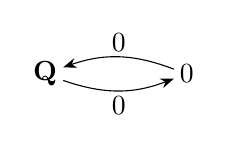
\begin{tikzpicture}[baseline=(current bounding box.center)]
      \node (Mstar) {$\QQ$};
      \node (M+)    [right=4em of Mstar] {$0$};
      \draw [arr, bend right=20] (Mstar) to node [below] {$0$} (M+);
      \draw [arr, bend right=20] (M+) to node [above] {$0$} (Mstar);
    \end{tikzpicture}
  \end{center}

\subsection{(Limits of) Discrete series representations}

  \noindent{\bf The Harish-Chandra module.}
  For $\ell \ge 0$, let $D_\ell = D_\ell^+ \oplus D_\ell^-$ be the direct sum of the $(\mathfrak{g},K)$-modules of the holomorphic and anti-holomorphic (limits of) discrete series representations on which $C$ acts via $\lambda=\ell^2$. This module is defined over $\QQ$ and is irreducible over $\QQ$. The components $D_\ell^\pm$ are defined over $\QQ[\sqrt{-1}]$ and are complex conjugate to each other. The lowest weight spaces $D_\ell^\pm[\chi_{\pm(\ell+1)}]$ are one-dimensional, while $D_\ell[\chi_{\pm(\ell-1)}]=0$.

  \smallskip\noindent{\bf The rational quiver representation.}
  Here, $M(\star) = 0$, so the maps $\phi_{a_\pm}, \phi_{b_\pm}$ are all zero. The operator $T_-$ acts as the identity on the one-dimensional space $D_\ell[\chi_{-(\ell+1)}]$, so unipotent stabilization is again trivial. This gives $\varphi_\star=0$ and $\varphi_\pm = c$.
  For $\ell \ge 1$, the associated $\QQ$-rational representation of the Gelfand quiver is:
  \begin{equation*}
    \begin{tikzcd}[column sep=large, row sep=large]
      \QQ[\sqrt{-1}] \arrow[r, arr, "0", bend left=10] \arrow[d, arr, "c"'] &
      0 \arrow[l, arr, "0", bend left=10] \arrow[r, arr, "0"', bend right=10] \arrow[d, arr, "0"] &
      \QQ[\sqrt{-1}] \arrow[l, arr, "0"', bend right=10] \arrow[d, arr, "c"] \\
      \QQ[\sqrt{-1}] \arrow[r, arr, "0", bend left=10] &
      0 \arrow[l, arr, "0", bend left=10] \arrow[r, arr, "0"', bend right=10] &
      \QQ[\sqrt{-1}] \arrow[l, arr, "0"', bend right=10]
    \end{tikzcd}
  \end{equation*}
  For $\ell = 0$, the Gelfand quiver degenerates to the cyclic quiver, and the diagram becomes:
  \begin{equation*}
    \begin{tikzcd}[column sep=large, row sep=large]
      \QQ[\sqrt{-1}] \arrow[r, arr, "0", bend left=10] \arrow[d, arr, "c"] & \QQ[\sqrt{-1}] \arrow[l, arr, "0", bend left=10] \arrow[d, arr, "c"] \\
      \QQ[\sqrt{-1}] \arrow[r, arr, "0", bend left=10] & \QQ[\sqrt{-1}] \arrow[l, arr, "0", bend left=10]
    \end{tikzcd}
  \end{equation*}
  
  \smallskip\noindent{\bf The \'etale $\QQ$-species representation.}
  For $\ell \ge 1$ (Gelfand quiver), the representation space over $\QQ$ is $W_{\{\star\}}=0$. The representation space over $\QQ[\sqrt{-1}]$ is $W_{\{\pm\}} = M(+)^{G_+} = \QQ[\sqrt{-1}]$. All maps are zero.
  \begin{center}
    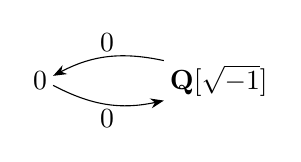
\begin{tikzpicture}[baseline=(current bounding box.center)]
      \node (Mstar) {$0$};
      \node (M+)    [right=4em of Mstar] {$\QQ[\sqrt{-1}]$};
      \draw [arr, bend right=20] (Mstar) to node [below] {$0$} (M+);
      \draw [arr, bend right=20] (M+) to node [above] {$0$} (Mstar);
    \end{tikzpicture}
  \end{center}
  For $\ell = 0$ (cyclic quiver), the associated species has one node with field $\QQ[\sqrt{-1}]$ and a twisted bimodule $\QQ[\sqrt{-1}]^{\rm twisted}$ (cf. Example \ref{ex:cyclic}). The representation is a one-dimensional $\QQ[\sqrt{-1}]$-vector space with a zero map
  \[
  f \colon \QQ[\sqrt{-1}] \otimes_{\QQ[\sqrt{-1}]} \QQ[\sqrt{-1}]^{\rm twisted} \to \QQ[\sqrt{-1}].
  \]
  
  \subsection{Principal series representations}
  
  \noindent{\bf The Harish-Chandra module.}
  For $\ell>0$ and $\epsilon\in\{0,1\}$ such that $\ell\not\equiv\epsilon\pmod{2}$, let $P_{\ell,\epsilon}$ be the principal series representation induced from the character $\mathrm{sgn}^{\epsilon}|\cdot|^{\ell-1}$ of the standard Borel subgroup. It is defined over $\QQ$ and fits into a non-split short exact sequence
  \[
  0 \to D_\ell \to P_{\ell,\epsilon} \to F_{\ell+1} \to 0.
  \]
  All relevant $K$-type spaces, $P_{\ell,\epsilon}[\chi_{\pm(\ell\pm 1)}]$, are one-dimensional.
  The dual principal series representation $P_{\ell,\epsilon}^\vee$ fits into the sequence $0 \to F_{\ell+1} \to P_{\ell,\epsilon}^\vee \to D_\ell \to 0$.
  
  \smallskip\noindent{\bf The rational quiver representation.}
  For $P_{\ell,\epsilon}$, unipotent stabilization is trivial. We have $\varphi_\pm = c$ and $\varphi_\star = c \circ X_\star$. The maps from $M(\pm)$ to $M(\star)$ factor through the quotient $F_{\ell+1}$ and are thus non-zero isomorphisms. The maps from $M(\star)$ to $M(\pm)$ factor through the submodule $D_\ell$ and are thus zero. After choosing suitable bases, the representation diagram is:
  \begin{equation*}
    \begin{tikzcd}[column sep=large, row sep=large]
      \QQ[\sqrt{-1}] \arrow[r, arr, "0", bend left=10] \arrow[d, arr, "c"'] &
      \QQ[\sqrt{-1}] \arrow[l, arr, "=", bend left=10] \arrow[r, arr, "="', bend right=10] \arrow[d, arr, "c \circ X_\star"] &
      \QQ[\sqrt{-1}] \arrow[l, arr, "0"', bend right=10] \arrow[d, arr, "c"] \\
      \QQ[\sqrt{-1}] \arrow[r, arr, "0", bend left=10] &
      \QQ[\sqrt{-1}] \arrow[l, arr, "=", bend left=10] \arrow[r, arr, "="', bend right=10] &
      \QQ[\sqrt{-1}] \arrow[l, arr, "0"', bend right=10]
    \end{tikzcd}
  \end{equation*}
  For the dual representation $P_{\ell,\epsilon}^\vee$, the horizontal arrows are reversed:
  \begin{equation*}
    \begin{tikzcd}[column sep=large, row sep=large]
      \QQ[\sqrt{-1}] \arrow[r, arr, "=", bend left=10] \arrow[d, arr, "c"'] &
      \QQ[\sqrt{-1}] \arrow[l, arr, "0", bend left=10] \arrow[r, arr, "0"', bend right=10] \arrow[d, arr, "c \circ X_\star"] &
      \QQ[\sqrt{-1}] \arrow[l, arr, "="', bend right=10] \arrow[d, arr, "c"] \\
      \QQ[\sqrt{-1}] \arrow[r, arr, "=", bend left=10] &
      \QQ[\sqrt{-1}] \arrow[l, arr, "0", bend left=10] \arrow[r, arr, "0"', bend right=10] &
      \QQ[\sqrt{-1}] \arrow[l, arr, "="', bend right=10]
    \end{tikzcd}
  \end{equation*}
  
  \smallskip\noindent{\bf The \'etale $\QQ$-species representation.}
  For $P_{\ell,\epsilon}$, the representation spaces are
  \[
  W_{\{\star\}} = \QQ\quad\text{and}\quad W_{\{\pm\}} = \QQ[\sqrt{-1}].
  \]
  The map
  \[
  f_{\{\pm\},\{\star\}} \colon \QQ[\sqrt{-1}] \otimes_{\QQ[\sqrt{-1}]} \QQ[\sqrt{-1}] \to \QQ
  \]
  corresponds to the non-zero maps $\phi_{b_\pm}$ and is given by the trace $\mathrm{tr}_{\QQ[\sqrt{-1}]/\QQ}$. The map $f_{\{\star\},\{\pm\}}$ is zero.
  \begin{center}
    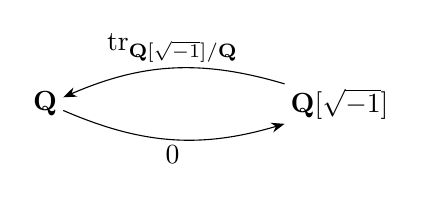
\begin{tikzpicture}[baseline=(current bounding box.center)]
      \node (Mstar) {$\QQ$};
      \node (M+)    [right=8em of Mstar] {$\QQ[\sqrt{-1}]$};
      \draw [arr, bend right=20] (Mstar) to node [below] {$0$} (M+);
      \draw [arr, bend right=20] (M+) to node [above] {$\mathrm{tr}_{\QQ[\sqrt{-1}]/\QQ}$} (Mstar);
    \end{tikzpicture}
  \end{center}
  For the dual representation $P_{\ell,\epsilon}^\vee$, the map
  \[
  f_{\{\star\},\{\pm\}} \colon \QQ \otimes_\QQ \QQ[\sqrt{-1}] \to \QQ[\sqrt{-1}]
  \]
  corresponds to the non-zero maps $\phi_{a_\pm}$ and is given by the canonical inclusion $\QQ \hookrightarrow \QQ[\sqrt{-1}]$, while $f_{\{\pm\},\{\star\}}$ is zero.
  \begin{center}
    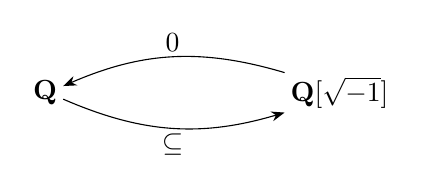
\begin{tikzpicture}[baseline=(current bounding box.center)]
      \node (Mstar) {$\QQ$};
      \node (M+)    [right=8em of Mstar] {$\QQ[\sqrt{-1}]$};
      \draw [arr, bend right=20] (Mstar) to node [below] {$\subseteq$} (M+);
      \draw [arr, bend right=20] (M+) to node [above] {$0$} (Mstar);
    \end{tikzpicture}
  \end{center}
  
    
    \begin{thebibliography}{99}

    \bibitem{ABR}
      C.~Alfes-Neumann, I.~Burban and M.~Raum.
      \newblock A classification of polyharmonic Maa\ss{} forms via quiver representations.
      \newblock {\em J. Algebra} \textbf{661} (2025),
      pages 713--756.

    \bibitem{DengDuParshallWang2008}
      B.~Deng, J.~Du, B.~Parshall, and J.~Wang.
      \newblock {\em Finite Dimensional Algebras and Quantum Groups}, volume 150 of {\em Mathematical Surveys and Monographs}.
      \newblock American Mathematical Society, Providence, RI, 2008.
      xxvi+759 pages.

    \bibitem{DlabRingel1975}
      V.~Dlab and C.M.~Ringel.
      \newblock On algebras of finite representation type.
      \newblock {\em J. Algebra}, {\bf 33} (1975),
      pages 306--394.

     \bibitem{DlabRingel1976}
       V.~Dlab and C.M.~Ringel.
       \newblock Indecomposable representations of graphs and algebras.
       \newblock {\em Memoirs of the American Mathematical Society}, {\bf 6}(173) (1973),
       v+57 pages.

    \bibitem{Gabriel1972}
      P.~Gabriel.
      \newblock Unzerlegbare Darstellungen. I.
      \newblock {\em Manuscr. Math.}, {\bf 6}(1) (1972),
      pages 71--103.

    \bibitem{HarderRaghuram-Book}
      G.~Harder and A.~Raghuram, \emph{Eisenstein Cohomology for $\mathrm{GL}_N$ and the Special Values of Rankin-Selberg $L$-Functions},
      \newblock Annals of Mathematics Studies, vol. 203, Princeton University Press, Princeton, NJ, 2019.
      240 pages.

    \bibitem{Harris2012}
      M.~Harris.
      \newblock Beilinson-Bernstein localization over {${\mathbb{Q}}$} and periods
      of automorphic forms.
      \newblock {\em Int. Math. Res. Not. IMRN {\bf 2013}},
      pages 2000--2053, 2013.
      
    \bibitem{Harris2020Erratum}
      M.~Harris.
      \newblock Beilinson--Bernstein Localization Over {Q} and Periods
      of Automorphic Forms: Erratum.
      \newblock {\em Int. Math. Res. Not. IMRN {\bf 2020}},
      pages 957--960, 2020.

    \bibitem{Januszewski18}
      F.~Januszewski.
      \newblock Rational Structures on Automorphic Representations.
      \newblock Math. Ann. {\bf 370} (2018),
      pages 1805--1881.

    %\bibitem{Ringel1976}
    %  C.~M.~ Ringel.
    %  \newblock Representations of $K$-species and bimodules.
    %  \newblock Journal of Algebra {\bf 41} (1976),
    %  269--302.
      
    \end{thebibliography}

\end{document}
